\documentclass[a4paper,12pt,oneside]{book}
\usepackage[left=2.5cm,right=2.5cm,top=2.5cm,bottom=2.5cm]{geometry}
\usepackage{graphicx}
\usepackage{amsmath}
\usepackage{amssymb}
\usepackage{amsfonts}
\usepackage{eufrak}
\usepackage{xcolor}
\newcommand{\red}[1]{{\color{red} #1}}
\newcommand{\blue}[1]{{\color{blue} #1}}
\newcommand{\magenta}[1]{{\color{magenta} #1}}
\newcommand{\brown}[1]{{\color{brown} #1}}
\definecolor{pinegreen}{rgb}{0.0, 0.47, 0.44}
\newcommand{\green}[1]{{\color{pinegreen} #1}}
\usepackage[utf8]{inputenc}
\usepackage{listings}
\usepackage{hyperref}
\usepackage{cancel}
\hypersetup{
    bookmarks=true,         % show bookmarks bar?
    unicode=false,          % non-Latin characters in Acrobat’s bookmarks
    pdftoolbar=true,        % show Acrobat’s toolbar?
    pdfmenubar=true,        % show Acrobat’s menu?
    colorlinks=true,        % false: boxed links; true: colored links
    linkcolor=red,          % color of internal links
    citecolor=green,        % color of links to bibliography
    filecolor=magenta,      % color of file links
    urlcolor=cyan           % color of external links
}

\DeclareUnicodeCharacter{039B}{\Lambda}
\DeclareUnicodeCharacter{03B4}{\delta}
\DeclareUnicodeCharacter{03B1}{\alpha}
\DeclareUnicodeCharacter{03B2}{\beta}

\newcommand{\veryshortarrow}[1][3pt]{\mathrel{%
   \hbox{\rule[\dimexpr\fontdimen22\textfont2-.2pt\relax]{#1}{.4pt}}%
   \mkern-4mu\hbox{\usefont{U}{lasy}{m}{n}\symbol{41}}}}

\newcommand{\NL}{\nonumber \\}
\newcommand{\nl}{\nonumber \\ & }
\newcommand{\beq}{\begin{equation}\begin{aligned}}
\newcommand{\eeq}{\end{aligned}\end{equation}}
\newcommand{\half}{\frac{1}{2}}
\newcommand{\quart}{\frac{1}{4}}
\newcommand{\op}{\hat}
\newcommand{\mat}{\mathbf}
\newcommand{\vect}{\mathbf}
\newcommand{\tnsr}{}
\newcommand{\snam}[1]{{\rm #1}}
\DeclareMathOperator{\sgn}{sgn}
\DeclareMathOperator{\trace}{tr}
\newcommand{\tbra}{\texttt{bra}}
\newcommand{\tket}{\texttt{ket}}
\newcommand{\perm}[1]{{\cal P}\left(#1\right)}
\newcommand{\Perm}[2]{{\cal P}\left({#1}\veryshortarrow {#2}\right)}
\newcommand{\sop}[1]{{\cal S}\left(#1\right)}
\newcommand{\Sop}[2]{{\cal S}\left(#1,#2\right)}
\newcommand{\asop}[1]{{\cal A}\left(#1\right)}
\newcommand{\ASop}[2]{{\cal A}\left(#1;#2\right)}
\newcommand{\eq}[1]{Eq.~(\ref{#1})}
\newcommand{\eqs}[2]{Eqs.~(\ref{#1},~\ref{#2})}
\newcommand{\sect}[1]{Sec.~\ref{#1}}
\newcommand{\spa}[1]{{#1}}
\newcommand{\spb}[1]{\bar{#1}}
\newcommand{\pos}[1]{{#1}^{+}}
\newcommand{\st}[1]{\mathfrak{#1}}
\newcommand{\dg}{\dagger}
\newcommand{\lk}{\left}
\newcommand{\rk}{\right}
\newcommand{\ieq}{\stackrel{!}{=}}
\newcommand{\elemcoil}{\textsf{ElemCo.jl}}
\newcommand{\quantwo}{\textsf{Quantwo} }
\newcommand{\cmd}[1]{\texttt{#1}}
\newcommand{\cdk}[1]{{\color{blue}{DK: #1}}}
\newcommand{\cks}[1]{{\color{green}{KS: #1}}}
% for presubscripts and presuperscripts (e.g., \pre{^x}U_a)
\newcommand{\pre}[1]{\,#1\!}
% Define \lt and \gt for `less than' and `greater than'
\mathchardef\lt="313C \mathchardef\gt="313E
% Set up `<' and `>' as angle brackets
\mathcode`<="4268 \mathcode`>="5269

\begin{document}
\title{Equations and derivations for \elemcoil}
\author{Daniel Kats, Charlotte Rickert, Thomas Schraivogel,\\ Denis Usvyat, Fangcheng Wu, Kristoffer Simula}
\maketitle
\tableofcontents
\chapter{Introduction}
\section{General}
In this document we collect the equations and derivations for methods implemented in the \elemcoil\ package.
The final goal is to have a document which can be used as a reference for the equations and derivations.
The final equations should also be contained in the code as docstrings or copied to the corresponding Markdown files.

\section{Notation} \label{sec:notation}

We use the following notation throughout the document.

The virtual orbitals are denoted by $a,b,c,\ldots$, the occupied orbitals by $i,j,k,\ldots$,
the active (open-shell) orbitals by $t,u,v,\ldots$,
and the general orbital indices are denoted by $p,q,r,s$.
The Einstein summation convention is used for repeated indices (repeated lower and upper indices are summed over).
The $\alpha$ and $\beta$ spin orbitals are denoted by $\spa{p}$ and $\spb{p}$.

The integrals are \textbf{not antisymmetrized} and denoted by $v_{pq}^{rs}$, where $p,q,r,s$ are indices of orbitals,
and the lower indices correspond to the creation and the upper indices to the annihilation operators in the Hamiltonian,
\begin{equation}
  \op H = E_0 + h_p^q \op a^\dagger_p \op a_q + 
  \frac{1}{2} v_{pq}^{rs} \op a^\dagger_p \op a^\dagger_q \op a_s \op a_r,
\end{equation}
or for the normal-ordered Hamiltonian,
\begin{equation}
  \op H_N = f_p^q \left\{\op a^\dagger_p \op a_q\right\}_N + 
  \frac{1}{2} v_{pq}^{rs} \left\{\op a^\dagger_p \op a^\dagger_q \op a_s \op a_r\right\}_N,
\end{equation}
i.e., $h_p^q = <p|\op h|q>$, $f_p^q = <p|\op f|q>$ and $v_{pq}^{rs} = <pq|rs>$.

Permutation operators:
\begin{equation}
\begin{aligned}
\perm{ab} X^{ij}_{ab} &= X^{ij}_{ba} \\
\Perm{ab}{ba} X^{ij}_{ab} &= X^{ij}_{ba} \\
\end{aligned}
\end{equation}

Symmetrization operators:
\begin{equation}
\begin{aligned}
\sop{ab} X^{ij}_{ab} &= X^{ij}_{ab} + X^{ij}_{ba}\\
\Sop{ab}{ij} X^{ij}_{ab} &= X^{ij}_{ab} + X^{ji}_{ba}\\
\end{aligned}
\end{equation}

Antisymmetrization operators:
\begin{equation}
\begin{aligned}
\asop{ab} X^{ij}_{ab} &= X^{ij}_{ab} - X^{ij}_{ba}\\
\ASop{ab}{ij} X^{ij}_{ab} &= X^{ij}_{ab} - X^{ji}_{ab} - X^{ij}_{ba} + X^{ji}_{ba}\\
\end{aligned}
\end{equation}


\chapter{Integrals}
\section{Density fitting and Cholesky decomposition}
\label{sec:df}
The electron-repulsion integrals in \elemcoil\ are obtained either from an external program 
through an FCIDUMP \cite{knowlesDeterminant1989} interface, 
or are calculated using the density-fitting approximation using an
interface to the \texttt{libcint}\cite{libcint} library.

In the density-fitting approximation, the electron-repulsion integrals are approximated by
\begin{equation}
  v_{pq}^{rs} \approx v_{p}^{rP} \left[v^{-1}\right]_{PQ} v_{q}^{sQ},
\end{equation}
where $v_{p}^{rP}$ and $v_{q}^{sQ}$ are density-fitted 3-index integrals with auxiliary 
basis functions $P,Q$, 
\begin{equation}
v_{p}^{rP} = \int d\vect{r}_1 d\vect{r}_2 \frac{\phi^*_p(\vect{r}_1) \phi^r(\vect{r}_1) \phi^P(\vect{r}_2)}{|\vect{r}_1-\vect{r}_2|},
\end{equation}
and $v^{PQ}$ is the Coulomb metric matrix,
\begin{equation}
  v^{PQ} = \int d\vect{r}_1 d\vect{r}_2 \frac{\phi^P(\vect{r}_1)\phi^Q(\vect{r}_2)}{|\vect{r}_1-\vect{r}_2|}.
\end{equation}

The Coulomb metric matrix is decomposed using the Cholesky factorization,
\begin{equation}
  v^{PQ} = \sum_L L^{P}_{L} L^{Q}_{L},
\end{equation}
where $L^{P}_{L}$ is a lower triangular matrix.
Thereafter, a non-symmetric square root of the inverse, $C_P^L$, is 
calculated by solving the equations
\begin{equation}
  L^{P}_{L'} C_{P}^{L} = \delta^{L}_{L'},
\end{equation}
with $\delta^{K}_{L}$ being the Kronecker delta. 
If $L^{P}_{L}$ is low-rank, the equation is solved using the QR decomposition,
otherwise it can be solved by simple back-substitution.

The transformed density-fitted integrals which are used throughout \elemcoil\ are 
then calculated by multiplying the density-fitted 3-index 
integrals with the non-symmetric square root of the inverse,
\begin{equation}
  v_{p}^{rL} = v_{p}^{rP} C_P^L,
\end{equation}
and the density-fitted 4-index integrals can be calculated by
\begin{equation}
  v_{pq}^{rs} \approx \sum_L v_{p}^{rL} v_{q}^{sL}.
  \label{eq:df_eri}
\end{equation}


\section{Frozen-core approximation}
\label{sec:frozen-core}
The frozen-core approximation is used to reduce the number of orbitals in the correlated 
calculation. The frozen-core approximation is implemented in \elemcoil\ by
setting the corresponding integrals to zero and adding their contribution to the
one-particle and zero-particle part of the Hamiltonian,
\begin{equation}
  \begin{aligned}
    \tilde h_p^q &= h_p^q + 2 v_{pI}^{qI} - v_{pI}^{Iq}\\
    \tilde E_0 &= E_0 + 2 h_I^I + 2 v_{IJ}^{IJ} - v_{IJ}^{JI},
  \end{aligned}
\end{equation}
where $\tilde h$ and $\tilde E_0$ denote the corrected one-body and zero-body terms, 
$I, J$ denote the core orbitals, and other indices do not include the core orbitals.
For the UHF Hamiltonian, the frozen-core approximation is implemented as
\begin{equation}
  \begin{aligned}
    \tilde h_{\spa p}^{\spa q} &= h_{\spa p}^{\spa q} + v_{\spa p \spa I}^{\spa q\spa I} + 
    v_{\spa p \spb I}^{\spa q\spb I} - v_{\spa p\spa I}^{\spa I\spa q}\\
    \tilde h_{\spb p}^{\spb q} &= h_{\spb p}^{\spb q} + v_{\spb p \spb I}^{\spb q\spb I} + 
    v_{\spb p \spa I}^{\spb q\spa I} - v_{\spb p\spb I}^{\spb I\spb q}\\
    \tilde E_0 &= E_0 + h_{\spa I}^{\spa I} + h_{\spb I}^{\spb I} + 
    \half\left(v_{\spa I\spa J}^{\spa I\spa J} + v_{\spb I\spb J}^{\spb I\spb J} 
    + 2 v_{\spa I\spb J}^{\spa I\spb J}
    - v_{\spa I\spa J}^{\spa J\spa I} - v_{\spb I\spb J}^{\spb J\spb I}
    \right).
  \end{aligned}
\end{equation}

If the frozen-core approximation is used in combination with the density-fitting approximation,
\textit{JKFIT} correction terms are added to the one-body and zero-body terms of the Hamiltonian in order to ensure that the
reference energy and the Fock matrix from DF-HF is not changed by the frozen-core approximation,
cf. \sect{sec:dfcorrection}.

\section{JKFIT/MPFIT correction} \label{sec:dfcorrection}
If the integrals are calculated using the density-fitting approximation using \textit{MPFIT}
fitting basis in \elemcoil, 
the correction terms are added using the \textit{JKFIT} fitting basis
to the one-body and zero-body terms of the Hamiltonian in order to ensure that the 
reference energy and the Fock matrix calculated using \textit{MPFIT}-fitted integrals
coincide with those from DF-HF (which employs the \textit{JKFIT} fitting basis), i.e.,
\begin{equation}
  \begin{aligned}
    \label{eq:df-correction}
    \tilde h_p^q &= \tilde f_p^q 
    - \sum_L \left(2v_{p}^{qL} v_{i}^{iL} - v_{p}^{iL} v_{i}^{qL}\right)\\
    \tilde E_0 &= E_0 + h_i^i - \tilde h_i^i + \tilde f_I^I, 
  \end{aligned} 
\end{equation}
where $\tilde h$ and $\tilde E_0$ denote the corrected one-body and zero-body terms,
\begin{equation}
  \begin{aligned}
    \label{eq:df-correction-fock}
    \tilde f_p^q &= h_p^q + \sum_{\tilde L} \left(2v_{p}^{q\tilde L} v_{\hat i}^{\hat i\tilde L} 
    - v_{p}^{\hat i\tilde L} v_{\hat i}^{q\tilde L}\right),
  \end{aligned} 
\end{equation}
and $I$ denotes the core orbitals (cf. \sect{sec:frozen-core}), 
$\hat i$ denote all occupied orbitals (including core)
and other indices do not include the core orbitals.
$\tilde L$ corresponds to the \textit{JKFIT} density-fitting basis functions,
and $L$ corresponds to the \textit{MPFIT} density-fitting basis functions.

\chapter{Hartree-Fock}
\section{Density-fitted Hartree-Fock}
The density-fitted Hartree-Fock equations are given by
\begin{equation}
\begin{aligned}
f_\mu^\nu C_\nu^p &= S_\mu^\nu C_\nu^p \epsilon_p\\
f_\mu^\nu &= h_\mu^\nu + 2\sum_L\left(v_{\mu'}^{iL} C^{\dagger\mu'}_i\right) C_{P}^{L} v_{\mu}^{\nu P}
- v_{\mu}^{iL} v^{\dagger\nu}_{iL}\\
v_{\mu}^{iL} &= \left(v_{\mu}^{\nu P} C_{\nu}^i\right) C_P^L.
\end{aligned}
\end{equation}
Alternatively, the $v_{\mu}^{\nu L}$ integrals can be precomputed and the Fock matrix can be calculated as
\begin{equation}
\begin{aligned}
f_\mu^\nu &= h_\mu^\nu + 2\sum_L\left(v_{\mu'}^{iL} C^{\dagger\mu'}_i\right) v_{\mu}^{\nu L}
- v_{\mu}^{iL} v^{\dagger\nu}_{iL}\\
v_{\mu}^{iL} &= v_{\mu}^{\nu L} C_{\nu}^i.
\end{aligned}
\end{equation}
Note that if the orbitals are real, $v^{\dagger\mu}_{iL} = v_{\mu}^{iL}$, 
and $C^{\dagger\mu}_i = C_{\mu}^i$.

The unrestricted Hartree-Fock equations are given (for $\alpha$ spin) by
\begin{equation}
\begin{aligned}
\pre{^\alpha}f_{\mu}^{\nu} C_{\nu}^{\spa p} &= S_{\mu}^{\nu} C_{\nu}^{\spa p} \epsilon_{\spa p}\\
\pre{^\alpha}f_{\mu}^{\nu} &= h_{\mu}^{\nu} + \sum_L\left(v_{\mu'}^{\spa i L} C^{\dagger\mu'}_{\spa i}
+v_{\mu'}^{\spb i L} C^{\dagger\mu'}_{\spb i}\right) C_{P}^{L} v_{\mu}^{\nu P}
- v_{\mu}^{\spa i L} v^{\dagger\nu}_{\spa i L}\\
v_{\mu}^{\spa i L} &= \left(v_{\mu}^{\nu P} C_{\nu}^{\spa i}\right) C_{P}^L,
\end{aligned}
\end{equation}
and equations for $\beta$ spin can be obtained by swapping the spins.

The residual of the Hartree-Fock equations, which can be used in DIIS, is given by 
\begin{equation}
\begin{aligned}
  \label{eq:hf-residual}
  \Delta f_{\mu}^{\nu} = S_{\mu}^{\nu'} D_{\nu'}^{\rho}f_{\rho}^{\nu} - f_{\mu}^{\nu'} D_{\nu'}^{\rho}S_{\rho}^{\nu},
  \quad \mbox{ with } \quad D_{\mu}^{\nu} = C_{\mu}^i C_i^{\dagger\nu}.
\end{aligned}
\end{equation}

\section{(Bi-orthogonal) Hartree-Fock}
The closed-shell Hartree-Fock on top of the FCIDUMP integrals (including the case of similarity-transformed 
Hamiltonians) is given by
\begin{equation}
\begin{aligned}
f_{\tilde p}^{\tilde q} C_{\tilde q}^p &= C_{\tilde p}^p \epsilon_p,\\
f_{\tilde p}^{\tilde q} &= h_{\tilde p}^{\tilde q} + 
\gamma^{\tilde r}_{\tilde s} \left(V_{\tilde p\tilde r}^{\tilde q\tilde s} 
- \half V_{\tilde p\tilde r}^{\tilde s\tilde q}\right),\\
  \gamma^{\tilde r}_{\tilde s} &= 2\sum_{i \in \rm occ} \bar C^{\dg \tilde r}_{i} C_{\tilde s}^i,
\end{aligned}
\end{equation}
where tilde indices correspond to the original orbitals.
If the FCIDUMP is similarity-transformed, $\bar C^{\dg \tilde r}_{p} \neq C_{\tilde r}^p$,
and $\bar C^{\dg \tilde r}_{p}$ are obtained as an inverse of $C_{\tilde r}^p$ such that
$\bar C^{\dg \tilde r}_{p} C_{\tilde r}^r = \delta^{r}_{p}$.

The unrestricted Hartree-Fock equations are given (for $\alpha$ case) by
\begin{equation}
\begin{aligned}
\pre{^\alpha}f_{\tilde p}^{\tilde q} C_{\tilde q}^{\spa p} &= C_{\tilde p}^{\spa p} \epsilon_{\spa p},\\
\pre{^\alpha}f_{\tilde p}^{\tilde q} &= h_{\tilde p}^{\tilde q} +
\left(\pre{^\alpha}\gamma^{\tilde r}_{\tilde s} + \pre{^\beta}\gamma^{\tilde r}_{\tilde s}\right) 
V_{\tilde p\tilde r}^{\tilde q\tilde s}
- \pre{^\alpha}\gamma^{\tilde r}_{\tilde s}V_{\tilde p\tilde r}^{\tilde s\tilde q},\\
\pre{^\alpha}\gamma^{\tilde r}_{\tilde s} &= \sum_{\spa i \in \rm occ} \bar C^{\dg \tilde r}_{\spa i} C_{\tilde s}^{\spa i},\\
\pre{^\beta}\gamma^{\tilde r}_{\tilde s} &=  \sum_{\spb i \in \rm occ} \bar C^{\dg \tilde r}_{\spb i} C_{\tilde s}^{\spb i},
\end{aligned}
\end{equation}
and equations for $\beta$ spin can be obtained by swapping the spins.
Note that if the FCIDUMP is of UHF type, the original indices and integrals are spin-dependent,
which has to be taken into account in the equations.

The residual of the Hartree-Fock equations, which can be used in DIIS, is equivalent to
\eq{eq:hf-residual}, with the overlap matrix $S_{\mu}^{\nu}$ removed.

\chapter{Density-Fitted Multiconfigurational Self-Consistent Field}
\section{Orbital Rotation}
The orbital transformed wavefunction can be expressed by
\begin{equation}
  |\Psi> = \exp(\hat{R})|0>,
\end{equation}
where
\begin{equation}
\begin{aligned}
  \exp(\hat{R}) &= 1+\hat{R}+\frac{1}{2!}\hat{R}^2+ \cdots, \\
  \hat{R} &= R_r^s\hat{E}_s^r,\\
\end{aligned}
\end{equation}

$\hat{E}^r_s$ is the singlet excitation operator $(\hat{a}_{r\alpha}^{\dagger}\hat{a}_{s\alpha}+\hat{a}_{r\beta}^{\dagger}\hat{a}_{s\beta} )$. 
Mathemetically if $\bf{R}$ is antisymmetric, $\exp(\hat{R})$ is an unitary transformation.
\begin{equation}
  \begin{aligned}
    R_r^s &= -R_s^r,\\
    \hat{R} &= [R_r^s(\hat{E}_s^r-\hat{E}_r^s)]_{r\mathchar"313E s},
  \end{aligned}
  \end{equation}

\section{MCSCF}
The energy expectation value of the wavefunction is be given by
\begin{equation}
\begin{aligned}
E(\bf{R}) &= <\Psi|\hat{H}|\Psi> \\
&= <0|\exp(-\hat{R})\hat{H}\exp(\hat{R})|0> \\
&= <0|\hat{H}|0> + <0|[\hat{H},\hat{R}]|0> + \frac{1}{2!}< 0|[[\hat{H},\hat{R}], \hat{R}]|0> + \cdots\\
&= E_0+\bf{g}^T\bf{x} +\frac{1}{2} \bf{x}^T\bf{hx}+ \cdots.\\
\end{aligned}
\end{equation}
In which Hamiltonian operator $\hat{H}$ is expressed as
\begin{equation}
\begin{aligned}
\hat{H} &= E_0 + h^q_p\hat{a}_p^\dagger\hat{a}_q + \frac{1}{2}v^{qs}_{pr}\hat{a}_p^\dagger\hat{a}_r^\dagger\hat{a}_s\hat{a}_q\\
&= E_0 + h^q_p\hat{E}^p_q + \frac{1}{2}v^{qs}_{pr}\hat{e}^{pr}_{qs},\\
\end{aligned}
\end{equation}
with $\hat{e}^{pr}_{qs}$ as the 2-electron excitation operator $\sum_{\sigma\tau}\hat{a}_{p\sigma}^\dagger\hat{a}_{r\tau}^\dagger\hat{a}_{s\tau}\hat{a}_{q\sigma}$.
In the first expression, $p,q,r,s$ denote the spin orbitals, and in the second expression, $p,q,r,s$ denote spatial orbitals.

The orbital transformation parameters $\bf{R}$ is expressed as vector $\bf{x}$, 
the linear coefficients as gradient vector $\bf{g}$, 
the quadratic coefficients as matrix $\bf{h}$. 
When terms after the quadratic terms truncated, 
to minimize the energy expectation value, the Lagrangian equation as known as the Newton-Raphson equation is
\begin{equation}
\frac{\partial}{\partial \bf{x}}(\bf{g}^T\bf{x}+\frac{1}{2}\bf{x}^T\bf{hx})= \bf{g}+\bf{hx} =0.
\end{equation}
Since the internal rotation of each of doubly occupied orbitals and virtual orbitals don't change the wavefunction, 
vector $\bf{x}$ is consisted of 4 parts, can be expressed as $[\bf{x}_t^j,\bf{x}_a^j,\bf{x}_t^u, \bf{x}_a^u]$.

Here, $\bf{g}$ is calculated from
\begin{equation}
\begin{aligned}
  g_r^k&= (\frac{\partial E}{\partial x_r^k})_{\bf{R = \bf{0}}}\\
  &= <0|[\hat{H}, \hat{E}^r_k-\hat{E}^k_r]|0>\\
  &= [1-\perm{rk}]<0|[\hat{E}^k_r, h^{q'}_{p'}\hat{E}^{p'}_{q'} + \frac{1}{2}v^{q's'}_{p'r'}\hat{e}^{p'r'}_{q's'}]|0>\\
  &= [1-\perm{rk}]<0|h^{q'}_r\hat{E}^k_{q'}-h^k_{p'}\hat{E}^{p'}_r +v^{q's'}_{rr'}\hat{e}^{kr'}_{q's'}- v^{ks'}_{p'r'}\hat{e}^{p'r'}_{rs'}|0>,\\
  &= [1-\perm{rk}](h^{q'}_r\pre{^1}D^k_{q'}-h^k_{p'}\pre{^1}D^{p'}_r+v^{q's'}_{rr'}\pre{^2}D^{kr'}_{q's'}-v^{ks'}_{p'r'}\pre{^2}D^{p'r'}_{rs'})
\end{aligned}
\end{equation}
let
\begin{equation}
  \red{A_r^k= \frac{1}{2}(h^{q'}_r\pre{^1}D^k_{q'} + h^r_{p'}\pre{^1}D^{p'}_k) + \frac{1}{2}(v^{q's'}_{rr'}\pre{^2}D^{kr'}_{q's'}+v^{rs'}_{p'r'}\pre{^2}D^{p'r'}_{ks'}),}
\end{equation}
then
\begin{equation}
  \red{g_r^k = 2(A_r^k-A_k^r).}
\end{equation}
In which 1-particle density matrix $\bf{\pre{^1}D}$ and 2-particle density matrix $\bf{\pre{^2}D}$ are defined as 
\begin{equation}
\begin{aligned}
  \pre{^1}D^t_u &= <0|\hat{E}^t_u|0> = c_Ic_J<\Phi_I|\hat{E}^t_u|\Phi_J>,\\
  \pre{^2}D^{tv}_{uw} &= <0|\hat{e}^{tv}_{uw}|0> = c_Ic_J<\Phi_I|\hat{e}^{tv}_{uw}|\Phi_J>.
\end{aligned}
\end{equation}
In order to simplify the expression, 
the $\pre{^1}D_v^u$ is written as $D_v^u$, and $\pre{^2}D_{tv}^{uw}$ is written as $D_{tv}^{uw}$ in follow. 

Fock matrix can be generalizingly defined as 
\begin{equation}
  F_r^s = \pre{^c}F_r^s + D^t_u[v^{su}_{rt}-\frac{1}{2}v^{us}_{rt}],
\end{equation}
with 
\begin{equation}
  \pre{^c}F_r^s = h^s_r+(2v^{sj}_{rj}-v^{js}_{rj})
\end{equation}
defined as the closed shell part of Fock matrix.

$\bf{A}_r^k$ can be calculated as 
\begin{equation}
\begin{aligned}
  A_r^i=& \frac{1}{2}(h^{q'}_rD^i_{q'} + h^r_{p'}D^{p'}_i) + \frac{1}{2}(v^{q's'}_{rr'}D^{ir'}_{q's'}+v^{rs'}_{p'r'}D^{p'r'}_{is'}),\\
  =&\frac{1}{2}(h^i_rD^i_i+h^r_iD^i_i)+\frac{1}{2}(v^{ij}_{rj}D^{ij}_{ij}+v^{rj}_{ij}D^{ij}_{ij} +v^{ji}_{rj}D^{ij}_{ji} +v^{rj}_{ji}D^{ji}_{ij}\\
    &+ v^{iu}_{rt}D^{it}_{iu}+v_{iu}^{rt}D_{it}^{iu} + v^{ui}_{rt}D^{it}_{ui} + v^{rt}_{ui}D^{ui}_{it})\\
  =&\frac{1}{2}(2h^i_r+2h^r_i)+\frac{1}{2}(4v^{ij}_{rj}+4v^{rj}_{ij} -2v^{ji}_{rj} -2v^{rj}_{ji} + 2v^{iu}_{rt}D^t_u+2v_{iu}^{rt}D_t^u - v^{ui}_{rt}D^t_u - v^{rt}_{ui}D^u_t)\\
  =&\sop{ri}(h^i_r+2v^{ij}_{rj}-v^{ji}_{rj}+v^{iu}_{rt}D^t_u-\frac{1}{2}v^{ui}_{rt}D^t_u)\\
  =&\sop{ri} F_r^i,
\end{aligned}
\end{equation}

\begin{equation}
\begin{aligned}
  A_r^u=& \frac{1}{2}(h^{q'}_rD^u_{q'} + h^r_{p'}D^{p'}_u) + \frac{1}{2}(v^{q's'}_{rr'}D^{ur'}_{q's'}+v^{rs'}_{p'r'}D^{p'r'}_{us'})\\
  =&\frac{1}{2}(h^t_rD^u_t+h^r_tD^t_u) + \frac{1}{2}(v^{tj}_{rj}D^{uj}_{tj}+v^{rj}_{tj}D^{tj}_{uj}+v^{tv}_{rw}D^{uw}_{tv}+v^{rw}_{tv}D^{tv}_{uw}+v^{jt}_{rj}D^{uj}_{jt}+v^{rj}_{jt}D^{jt}_{uj})\\
  =&\frac{1}{2}(h^t_rD^u_t+h^r_tD^t_u) + \frac{1}{2}(2v^{tj}_{rj}D^u_t+2v^{rj}_{tj}D^t_u+v^{tv}_{rw}D^{uw}_{tv}+v^{rw}_{tv}D^{tv}_{uw}-v^{jt}_{rj}D^u_t-v^{rj}_{jt}D^t_u)\\
  =&\frac{1}{2}[(h^t_r + 2v^{tj}_{rj} - v^{jt}_{rj})D^u_t + v^{tv}_{rw}D^{uw}_{tv}] + \frac{1}{2}[(h^r_t + 2v^{rj}_{tj} - v^{jr}_{tj})D^t_u + v^{rw}_{tv}D^{tv}_{uw}]\\
  =&\frac{1}{2}(\pre{^c}F_r^tD^u_t+v^{tv}_{rw}D^{uw}_{tv}) + \frac{1}{2}(\pre{^c}F_t^rD^t_u+v^{rw}_{tv}D^{tv}_{uw}),\\
\end{aligned}
\end{equation}

\begin{equation}
  A_r^a=0.
\end{equation}

Electronic energy $E$ after orbital transformation is calculated with transformed orbitals and active orbital 1- and 2-particle density matrices
\begin{equation}
E=\pre{^c}F_t^uD^t_u+\frac{1}{2}v^{uw}_{tv}D^{tv}_{uw}+E_c,
\end{equation}
with
\begin{equation}
  E_c=h^j_j+\pre{^c}F_j^j,
\end{equation}
$E_c$ is the closed shell electronic energy.

The 4-index integral $v^{uw}_{tv}$ is calculated as the density fitted integrals, as mentioned in previous chapter,
\begin{equation}
\begin{aligned}
  v^{uw}_{tv} =& v^{uL}_t v^{wL}_v,\\
  v^{uL}_t =& v^{\nu L}_{\mu} C_t^{\dagger \mu} C^u_{\nu}.\\
\end{aligned}
\end{equation}
Likewise, other four-index integrals in this chapter are calculated in the same way.


\section{Augmented Hessian}
In order to make the coefficients transforming step smaller and more robust, 
a level-shift $\epsilon$ is introduced to control the step $\bf{x}$ \cite{augmentedHessian1981}
\begin{equation}
\bf{g}+(\bf{h}+\epsilon \bf{I})\bf{x}=0,
\end{equation}
in which
\begin{equation}
\epsilon =-\lambda^2\bf{x}^T\bf{g},
\end{equation}
\begin{equation}
\begin{pmatrix}
    0 & \lambda \bf{g}^T \\
    \lambda \bf{g} & \bf{h}
\end{pmatrix}
\begin{pmatrix}
    \frac{1}{\lambda} \\
    \bf{x}
\end{pmatrix}
= \nu
\begin{pmatrix}
    \frac{1}{\lambda} \\
    \bf{x}
\end{pmatrix}.
\end{equation}

We search for the value of $\lambda$ with a combination method of linear search and logarithmic bisection search:
\begin{equation}
\begin{aligned}
  \lambda =&\frac{(\left\lVert\bf{x_{small\lambda}}\right\rVert - trust) + (trust -\left\lVert\bf{x_{large\lambda}}\right\rVert)}{\left\lVert\bf{x_{small\lambda}}\right\rVert-\left\lVert\bf{x_{large\lambda}}\right\rVert},\\
  \lambda=&\exp{(\ln{small\lambda}+(\ln{big\lambda}-\ln{small\lambda}) * bisecdamp)}.
\end{aligned}
\end{equation}
If there are both tested smallest and biggest limits in one iteration search for $\lambda$, we adopt the linear search with the norm of both limit $\bf{x}$,
otherwise, we use either the upper and lower boundaries value(by default set to be 1000 and 1) and the tested $\lambda$ to do the logarithmic bisection search.


\section{Hessian Approximation}

\subsection{First Order Approximation}
We adopt the Super-CI optimization approximation\cite{SCI1989}, in which 
\begin{equation}
\hat{H}^{eff}=\sum_{pq}F_p^q \hat{E}_p^q,
\end{equation}
\begin{equation}
E^{(0)}=<0|\hat{H}^{eff}|0>,
\end{equation}
\begin{equation}
\pre{^{SCI}}H_{rs}^{kl}=2<rk|\hat{H}^{eff} - E^{(0)}|sl>.
\end{equation}
More specifically,
\begin{equation}
\begin{aligned}
  \red{\pre{^{SCI}}H_{ab}^{ij} =}&\red{ 4(\delta_i^j F_a^b-\delta_a^b F_i^j),}\\
  \red{\pre{^{SCI}}H_{ab}^{iu} =}&\red{ -2\delta_a^b F_i^vD_v^u,} \\
  \red{\pre{^{SCI}}H_{au}^{ij} =}&\red{ \delta_i^j(4F_a^u-2F_a^vD_v^u), }\\
  \red{\pre{^{SCI}}H_{tb}^{iu} =}&\red{ 0,}\\
  \red{\pre{^{SCI}}H_{tu}^{ij} =}&\red{ (2D_t^u-4\delta_t^u) F_i^j+2\delta_i^j[2F_t^u-(D^{tv}_{uw}-D^t_uD^v_w)F_v^w-D_t^vF_v^u-F_t^vD^v_u],}\\
  \red{\pre{^{SCI}}H_{ab}^{tu} =}&\red{ 2\delta^a_b (D^{tv}_{uw}-D^t_uD^v_w)F_v^w + 2D^t_uF_a^b.}
\end{aligned}
\end{equation}

\subsection{Second Order Approximation}
In general, the second-order Hessian matrix elements are calculated as
\begin{equation}
\begin{aligned}
  \pre{^{SO}}H_{rs}^{kl} =&  (\frac{\partial E}{\partial x_r^k\partial x_s^l})_{\bf{R = \bf{0}}}\\
  =& \frac{1}{2}\Sop{rs}{kl} <0|[[\hat{H},\hat{E}^k_r-\hat{E}^r_k],\hat{E}^l_s-\hat{E}^s_l]|0>\\
  =& \frac{1}{2}\Sop{rs}{kl} \ASop{rk}{sl} <0|[[\hat{H},\hat{E}^k_r], \hat{E}^l_s]|0>\\
  =& \frac{1}{2}\Sop{rs}{kl} \ASop{rk}{sl} <0|[\hat{E}^l_s,[\hat{E}^k_r, h^{q'}_{p'}\hat{E}^{p'}_{q'} + \frac{1}{2}v^{q's'}_{p'r'}\hat{e}^{p'r'}_{q's'}]]|0>\\
  =& \frac{1}{2}\Sop{rs}{kl} \ASop{rk}{sl} (-h^l_rD^k_s -h^k_sD^l_r + h^{q'}_rD^l_{q'}\delta^k_s + h^k_{p'}D^{p'}_s\delta^l_r\\
  &+\delta^k_sv^{q's'}_{rr'}D^{lr'}_{q's'} + \delta^l_r v^{ks'}_{p'r'}D^{p'r'}_{ss'}-v^{ls'}_{rr'}D^{kr'}_{ss'} - v^{ks'}_{sr'}D^{lr'}_{rs'}\\
  &+v^{q's'}_{rs}D^{kl}_{q's'} + v^{kl}_{p'r'}D^{p'r'}_{rs} - v^{q'l}_{rr'}D^{kr'}_{q's} - v^{ks'}_{p's}D^{p'l}_{rs'})\\
  =& \ASop{rk}{sl} (-h^l_rD^k_s - h^k_sD^l_r -v^{ls'}_{rr'}D^{kr'}_{ss'} - v^{ks'}_{sr'}D^{lr'}_{rs'} +v^{q's'}_{rs}D^{kl}_{q's'} + v^{kl}_{p'r'}D^{p'r'}_{rs} - v^{q'l}_{rr'}D^{kr'}_{q's} - v^{ks'}_{p's}D^{p'l}_{rs'} )\\
   &+ \frac{1}{2} \Sop{rs}{kl} \ASop{rk}{sl} \delta^k_s(h^{q'}_rD^l_{q'} + h^r_{p'}D^{p'}_l +v^{q's'}_{rr'} D^{lr'}_{q's'}+ v^{rs'}_{p'r'}D^{p'r'}_{ls'} ) \\
  =&\red{ \ASop{rk}{sl} (h^s_rD^k_l + h^r_s D^l_k + v^{ss'}_{rr'}D^{kr'}_{ls'} + v^{rs'}_{sr'}D^{lr'}_{ks'} + v^{q's'}_{rs}D^{kl}_{q's'} + v^{rs}_{p'r'}D^{p'r'}_{kl} + v^{q's}_{rr'}D^{kr'}_{q'l}+  v^{rs'}_{p's}D^{p'l}_{ks'}) }\\
   &+ \ASop{rk}{sl}(\delta^k_sA^l_r+\delta^l_rA^k_s)\\
  =& \ASop{rk}{sl} [2G^{kl}_{rs}+ \red{\delta^k_s(A^l_r+A^r_l)}]\\
  =& \ASop{rk}{sl} [2G^{kl}_{rs}-\delta^k_l(A_r^s+A_s^r)],\\
\end{aligned}
\end{equation}
matrices $\bf{G}$ are defined as
\begin{equation}
  \red{G^{kl}_{rs} = \frac{1}{2} (h^s_rD^k_l + h^r_s D^l_k + v^{ss'}_{rr'}D^{kr'}_{ls'} + v^{rs'}_{sr'}D^{lr'}_{ks'} + v^{q's'}_{rs}D^{kl}_{q's'} + v^{rs}_{p'r'}D^{p'r'}_{kl} + v^{q's}_{rr'}D^{kr'}_{q'l}+  v^{rs'}_{p's}D^{p'l}_{ks'})}
\end{equation}

\begin{equation}
\red{G^{ij}_{rs} = \delta_i^j(F^r_s+F^s_r)+L^{ij}_{rs} + L^{rs}_{ij},}
\end{equation}
\begin{equation}
\red{G^{tj}_{rs} = \frac{1}{2}(D^t_uL^{uj}_{rs} + D^u_tL^{rs}_{uj}) = G^{jt}_{sr},}
\end{equation}
\begin{equation}
\red{G^{tu}_{rs} = \frac{1}{2}( \pre{^c}F_r^sD_t^u + \pre{^c}F_s^rD_u^t  + v^{sw}_{rv}D^{tv}_{uw} + v^{rv}_{sw}D^{uw}_{tv})+v^{vw}_{rs}D^{tu}_{vw} + v_{vw}^{rs}D_{tu}^{vw},}
\end{equation}
where
\begin{equation}
  L^{pq}_{rs} = 2v^{pq}_{rs} +2^{ps}_{rq} - v^{sp}_{rq} - v^{qp}_{rs}.
\end{equation}

\subsection{Combined Second-Order and Super-CI Hessian Approximation}
By default, the SO-SCI Hessian matrix \cite{kreplinMCSCF2020} is approximated as below:
\begin{equation}
\begin{aligned}
\pre{^{SO-SCI}}H_{ab}^{ij} =& \pre{^{SCI}}H_{ab}^{ij},\\
\pre{^{SO-SCI}}H_{ab}^{iu} =& \pre{^{SCI}}H_{ab}^{iu},\\
\pre{^{SO-SCI}}H_{au}^{ij} =& \pre{^{SCI}}H_{au}^{ij},\\
\pre{^{SO-SCI}}H_{tb}^{iu} =& \pre{^{SO}}H_{tb}^{iu},\\
\pre{^{SO-SCI}}H_{tu}^{ij} =& \pre{^{SO}}H_{tu}^{ij},\\
\pre{^{SO-SCI}}H_{ab}^{tu} =& \pre{^{SO}}H_{ab}^{tu}.\\
\end{aligned}
\end{equation}
If the $\bf{SO\_SCI\_origin}$ option is set to be $false$, 
\begin{equation}
  \pre{^{SO-SCI}}H_{ab}^{tu} = \pre{^{SCI}}H_{ab}^{tu},
\end{equation}
and the rest blocks of Hessian matrix remain the same.

\chapter{MP2: Second-Order M{\o}ller--Plesset Perturbation Theory}
\label{ch:mp2}

\section{Spin-Orbital Formulation}
\label{sec:spin-orbital-mp2}

In the spin-orbital basis, the MP2 correlation energy is
\begin{equation}
\label{eq:spin-orbital-mp2}
E^{(2)} = \frac{1}{4} \sum_{IJAB} \frac{(v_{IJ}^{AB} - v_{IJ}^{BA})(v^{IJ}_{AB} - v^{IJ}_{BA})}
{\varepsilon_I + \varepsilon_J - \varepsilon_A - \varepsilon_B},
\end{equation}
where $I,J,A,B$ denote \emph{spin-orbitals}.
The factor $\tfrac{1}{4}$ compensates for unrestricted summation over equivalent 
excitations $(IJ \leftrightarrow JI, AB \leftrightarrow BA)$.


\section{Closed-Shell RHF--MP2}
\label{sec:rhf-mp2}

For a closed-shell RHF reference, $\alpha$ and $\beta$ electrons occupy 
the same spatial orbitals with identical orbital energies. We sum over 
spin explicitly.

\subsection{Spin Cases}
The integral $v_{i_{\sigma_1} j_{\sigma_2}}^{a_{\sigma_3} b_{\sigma_4}}$
is nonzero only when $\sigma_1 = \sigma_3$ and $\sigma_2 = \sigma_4$ (spin conservation).

\paragraph{Same-spin ($\alpha\alpha$ and $\beta\beta$).}
Both direct and exchange terms survive:
\begin{equation}
v_{i_\alpha j_\alpha}^{a_\alpha b_\alpha} - v_{i_\alpha j_\alpha}^{b_\alpha a_\alpha} 
= v_{ij}^{ab} - v_{ij}^{ba}.
\end{equation}

\paragraph{Opposite-spin ($\alpha\beta$ and $\beta\alpha$).}
The exchange term vanishes by spin orthogonality:
\begin{equation}
v_{i_\alpha j_\beta}^{a_\alpha b_\beta} = v_{ij}^{ab}.
\end{equation}

\subsection{Spin Summation}
Denoting $\Delta_{IJAB} = \varepsilon_I + \varepsilon_J - \varepsilon_A - \varepsilon_B$
and converting to spatial orbitals, we must account for overcounting.

\paragraph{Same-spin ($\alpha\alpha + \beta\beta$).}
Each spatial configuration $(i,j,a,b)$ appears 4 times in the spin-orbital sum
(swapping $i \leftrightarrow j$ and $a \leftrightarrow b$). With two identical 
spin cases and the $\tfrac{1}{4}$ factor:
\begin{equation}
E^{(2)}_{\alpha\alpha} + E^{(2)}_{\beta\beta} 
= 2 \times \frac{1}{4} \sum_{ijab} \frac{(v_{ij}^{ab} - v_{ij}^{ba})(v_{ab}^{ij} - v_{ba}^{ij})}{\Delta_{ijab}}.
\end{equation}

\paragraph{Opposite-spin ($\alpha\beta + \beta\alpha$).}
Each spatial configuration appears twice (swapping both pairs simultaneously).
With two identical spin cases:
\begin{equation}
E^{(2)}_{\alpha\beta} + E^{(2)}_{\beta\alpha} 
= 2 \times \frac{1}{2} \sum_{ijab} \frac{v_{ij}^{ab}v_{ab}^{ij}}{\Delta_{ijab}}.
\end{equation}

\subsection{Expanding the Same-Spin Term}
Expand the squared antisymmetric integral:
\begin{equation}
(v_{ij}^{ab} - v_{ij}^{ba})(v^{ij}_{ab} - v^{ij}_{ba}) 
= v_{ij}^{ab}v^{ij}_{ab} - v_{ij}^{ab}v^{ij}_{ba} - v_{ij}^{ba}v^{ij}_{ab} + v_{ij}^{ba}v^{ij}_{ba}.
\end{equation}
Since $\sum_{ijab} v_{ij}^{ba}v^{ij}_{ba} = \sum_{ijab} v_{ij}^{ab}v^{ij}_{ab}$ 
by relabeling $a \leftrightarrow b$:
\begin{equation}
\sum_{ijab} (v_{ij}^{ab} - v_{ij}^{ba})(v^{ij}_{ab} - v^{ij}_{ba}) 
= 2 \sum_{ijab} \bigl(v_{ij}^{ab}v^{ij}_{ab}  - v_{ij}^{ab}v^{ij}_{ba}\bigr).
\end{equation}

\subsection{SS and OS Contributions}
Substituting the expansion into the same-spin term:
\begin{equation}
E^{(2)}_{\mathrm{SS}} = \frac{1}{2} \cdot 2 \sum_{ijab} 
  \frac{v_{ij}^{ab}v^{ij}_{ab}  - v_{ij}^{ab}v^{ij}_{ba}}{\Delta_{ijab}}
= \sum_{ijab} \frac{v_{ij}^{ab}(v_{ab}^{ij} - v_{ba}^{ij})}{\Delta_{ijab}}.
\end{equation}
The opposite-spin contribution simplifies to:
\begin{equation}
E^{(2)}_{\mathrm{OS}} = \sum_{ijab} \frac{v_{ij}^{ab}v_{ab}^{ij}}{\Delta_{ijab}}.
\end{equation}

\subsection{Final RHF--MP2 Formula}
Adding SS and OS:
\begin{equation}
\begin{aligned}
E^{(2)}_{\mathrm{RHF}} &= E^{(2)}_{\mathrm{SS}} + E^{(2)}_{\mathrm{OS}} \\[4pt]
&= \sum_{ijab} \frac{v_{ij}^{ab}(v_{ab}^{ij} - v_{ba}^{ij}) 
   + v_{ij}^{ab}v_{ab}^{ij}}{\Delta_{ijab}}.
\end{aligned}
\end{equation}
Factoring:
\begin{equation}
\label{eq:rhf-mp2}
\boxed{E^{(2)}_{\mathrm{RHF}} = \sum_{ijab} 
\frac{v_{ij}^{ab} (2v_{ab}^{ij} - v_{ba}^{ij})}{\Delta_{ijab}}.}
\end{equation}

\subsection{Amplitude Form}
Using spatial-orbital amplitudes $T^{ij}_{ab} = v_{ab}^{ij} / \Delta_{ijab}$:
\begin{equation}
\begin{aligned}
E^{(2)}_{\mathrm{SS}} &= \sum_{ijab} v_{ij}^{ab} (T^{ij}_{ab} - T^{ij}_{ba}), \\
E^{(2)}_{\mathrm{OS}} &= \sum_{ijab} v_{ij}^{ab} \, T^{ij}_{ab}, \\
E^{(2)}_{\mathrm{RHF}} &= \sum_{ijab} v_{ij}^{ab} (2T^{ij}_{ab} - T^{ij}_{ba}).
\end{aligned}
\end{equation}


\section{Unrestricted UHF--MP2}
\label{sec:uhf-mp2}

For UHF, $\alpha$ and $\beta$ electrons occupy \emph{different} spatial orbitals 
with different orbital energies. We use $(\spa{i},\spa{j},\spa{a},\spa{b})$ for $\alpha$ 
and $(\spb{i},\spb{j},\spb{a},\spb{b})$ for $\beta$.

\subsection{Three Spin Contributions}
\begin{equation}
E^{(2)}_{\mathrm{UHF}} = E^{(2)}_{\alpha\alpha} + E^{(2)}_{\beta\beta} + E^{(2)}_{\alpha\beta}.
\end{equation}

\paragraph{Same-spin $\alpha\alpha$.}
With antisymmetrized integrals and antisymmetric amplitudes:
\begin{equation}
E^{(2)}_{\alpha\alpha} = \frac{1}{4} \sum_{\spa{i}\spa{j}\spa{a}\spa{b}}
\frac{(v_{\spa{i}\spa{j}}^{\spa{a}\spa{b}} - v_{\spa{i}\spa{j}}^{\spa{b}\spa{a}})(v^{\spa{i}\spa{j}}_{\spa{a}\spa{b}} - v^{\spa{i}\spa{j}}_{\spa{b}\spa{a}})}{\Delta_{\spa{i}\spa{j}\spa{a}\spa{b}}}
= \frac{1}{2} \sum_{\spa{i}\spa{j}\spa{a}\spa{b}} v_{\spa{i}\spa{j}}^{\spa{a}\spa{b}} \, T^{\spa{i}\spa{j}}_{\spa{a}\spa{b}}.
\end{equation}
The $\tfrac{1}{4} \to \tfrac{1}{2}$ follows from amplitude antisymmetry.

\paragraph{Same-spin $\beta\beta$.}
\begin{equation}
E^{(2)}_{\beta\beta} = \frac{1}{2} \sum_{\spb{i}\spb{j}\spb{a}\spb{b}} v_{\spb{i}\spb{j}}^{\spb{a}\spb{b}} \, T^{\spb{i}\spb{j}}_{\spb{a}\spb{b}}.
\end{equation}

\paragraph{Opposite-spin $\alpha\beta$.}
No exchange, no antisymmetry, no overcounting:
\begin{equation}
E^{(2)}_{\alpha\beta} = \sum_{\spa{i}\spb{j}\spa{a}\spb{b}} \frac{v_{\spa{i}\spb{j}}^{\spa{a}\spb{b}}v^{\spa{i}\spb{j}}_{\spa{a}\spb{b}}}{\Delta_{\spa{i}\spb{j}\spa{a}\spb{b}}}
= \sum_{\spa{i}\spb{j}\spa{a}\spb{b}} v_{\spa{i}\spb{j}}^{\spa{a}\spb{b}} \, T^{\spa{i}\spb{j}}_{\spa{a}\spb{b}}.
\end{equation}

\subsection{Final UHF--MP2 Formula}
\begin{equation}
\label{eq:uhf-mp2}
\boxed{E^{(2)}_{\mathrm{UHF}} = \frac{1}{2} \sum_{\spa{i}\spa{j}\spa{a}\spa{b}} v_{\spa{i}\spa{j}}^{\spa{a}\spa{b}} \, T^{\spa{i}\spa{j}}_{\spa{a}\spa{b}}
+ \frac{1}{2} \sum_{\spb{i}\spb{j}\spb{a}\spb{b}} v_{\spb{i}\spb{j}}^{\spb{a}\spb{b}} \, T^{\spb{i}\spb{j}}_{\spb{a}\spb{b}}
+ \sum_{\spa{i}\spb{j}\spa{a}\spb{b}} v_{\spa{i}\spb{j}}^{\spa{a}\spb{b}} \, T^{\spa{i}\spb{j}}_{\spa{a}\spb{b}},}
\end{equation}
with amplitudes
\begin{equation}
\begin{aligned}
T^{\spa{i}\spa{j}}_{\spa{a}\spa{b}} &= \frac{v^{\spa{i}\spa{j}}_{\spa{a}\spa{b}} - v^{\spa{i}\spa{j}}_{\spa{b}\spa{a}}}
{\varepsilon_{\spa{i}} + \varepsilon_{\spa{j}} - \varepsilon_{\spa{a}} - \varepsilon_{\spa{b}}}, \\[4pt]
T^{\spb{i}\spb{j}}_{\spb{a}\spb{b}} &= \frac{v^{\spb{i}\spb{j}}_{\spb{a}\spb{b}} - v^{\spb{i}\spb{j}}_{\spb{b}\spb{a}}}
{\varepsilon_{\spb{i}} + \varepsilon_{\spb{j}} - \varepsilon_{\spb{a}} - \varepsilon_{\spb{b}}}, \\[4pt]
T^{\spa{i}\spb{j}}_{\spa{a}\spb{b}} &= \frac{v^{\spa{i}\spb{j}}_{\spa{a}\spb{b}}}
{\varepsilon_{\spa{i}} + \varepsilon_{\spb{j}} - \varepsilon_{\spa{a}} - \varepsilon_{\spb{b}}}.
\end{aligned}
\end{equation}

\subsection{Key Differences from RHF}
\begin{itemize}
  \item No factor of 2 on SS terms ($\alpha$ and $\beta$ orbitals differ).
  \item Separate integrals and orbital energies for each spin.
  \item No exchange in the OS contribution.
\end{itemize}


\chapter{Positron}

We consider systems with electrons and a single positron.
Positron orbital indices are marked with a superscript plus:
occupied positron orbitals $\pos{i},\pos{j},\pos{k},\ldots$,
virtual positron orbitals $\pos{a},\pos{b},\pos{c},\ldots$,
and general positron indices $\pos{p},\pos{q},\pos{r},\pos{s}$.
Electron indices remain undecorated as defined in \sect{sec:notation}.
We use $\op b^\dagger, \op b$ for positron creation and annihilation operators
to distinguish them from the electronic operators $\op a^\dagger, \op a$.

The full electron--positron Hamiltonian in second quantization reads
\begin{equation}
\op H = E_0 + h_p^q \op a^\dagger_p \op a_q
+ h_{\pos{p}}^{\pos{q}(\mathbf{+})} \op b^\dagger_{\pos{p}} \op b_{\pos{q}}
+ \frac{1}{2} v_{pq}^{rs} \op a^\dagger_p \op a^\dagger_q \op a_s \op a_r
- v_{p\pos{q}}^{r\pos{s}} \op a^\dagger_p \op b^\dagger_{\pos{q}} \op b_{\pos{s}} \op a_r,
\end{equation}
where $h_{\pos{p}}^{\pos{q}(\mathbf{+})}$ is the positron one--body Hamiltonian
(differing from the electronic one by the sign of the nuclear attraction),
$v_{p\pos{q}}^{r\pos{s}} = \langle p\pos{q}|r\pos{s}\rangle$ are the
electron--positron Coulomb integrals,
and the minus sign reflects the attractive electron--positron interaction.
With a single positron, any positron--positron repulsion term vanishes.

\section{Density fitting with positron}

With positrons, the density-fitted correction equations (\ref{eq:df-correction}) and (\ref{eq:df-correction-fock}) are modified to include the positron contributions:
\begin{equation}
  \begin{aligned}
    \tilde h_p^q &= \tilde f_p^q 
    - \sum_L \left(2v_{p}^{qL} v_{i}^{iL} - v_{p}^{iL} v_{i}^{qL} - v_{p}^{qL} v_{\pos{i}}^{\pos{i}L}
    \right)\\
    \tilde{f}_p^q &= h_p^q + \sum_{\tilde{L}} \left(2v_{p}^{q\tilde L} v_{\hat i}^{\hat i\tilde L} 
    - v_{p}^{\hat i\tilde L} v_{\hat i}^{q\tilde L} - v_{p}^{q\tilde L} v_{\pos{i}}^{\pos{i}\tilde L} \right),\\
  \end{aligned}
\end{equation}
where $\pos{i}=1$ denote the single occupied positron orbital,
$\hat i$ denote all occupied orbitals (including core), 
and $\tilde L$ denote the auxiliary basis functions. 
The positron one-body terms get corrections according to 
\begin{equation}
  \begin{aligned}
    \tilde h_{\pos{p}}^{\pos{q} (\mathbf{+})} &= \tilde f_{\pos{p}}^{\pos{q} (\mathbf{+})} 
    + \sum_L \left(2v_{i}^{iL}v_{\pos{p}}^{\pos{q}L}\right)\\
    \tilde f_{\pos{p} }^{\pos{q} (\mathbf{+})} &= h_{\pos{p}}^{\pos{q} (\mathbf{+})} - \sum_L \left(2v_{ \hat i}^{ \hat i \tilde L}v_{\pos{p}}^{\pos{q} \tilde L}\right), 
    \\
  \end{aligned}
\end{equation}
and the core energy is saved as
\begin{equation}
\tilde{E}_0 = E_0 + h_{i}^{i} + \tfrac12 h^{\pos{i}(\mathbf{+})}_{\pos{i}} - \left( \tilde h_{ i}^{ i} + \tfrac12 \tilde h^{\pos{i}(\mathbf{+})}_{\pos{i}}  \right).
\end{equation}

At the moment the positron integral evaluation does not support frozen-core approximation. 

\section{Positron Hartree--Fock}
\label{sec:positron-hf}

A closed--shell electron reference plus a single positron is formally
analogous to an \textit{unrestricted} HF problem with two spin blocks:
the $\alpha$ electrons and the positron ($e^+$). The key
difference is that the positron block contains \emph{exactly one}
occupied orbital, so there is no exchange term between two positrons.
Also there is an attractive Coulomb interaction between the positron and the
electrons instead of the repulsive one between $\alpha$ and $\beta$ electrons.  

\subsection{Density--fitted working equations}
The coupled Roothaan equations
\begin{equation}
f_{\mu}^{\nu(e)} C_{\nu}^{p} = S_{\mu}^{\nu} C_{\nu}^{p} \epsilon_{p},\qquad
f_{\mu}^{\nu(p)} C_{\nu}^{\pos{p}} = S_{\mu}^{\nu} C_{\nu}^{\pos{p}} \epsilon_{\pos{p}},
\label{eq:poshf-roothaan}
\end{equation}
are solved self--consistently.

With density fitting [cf.~\sect{sec:df}] we reuse the three--index
intermediates $v_{\mu}^{\nu L}$ and the metric factors $C_{P}^{L}$. The
AO density matrices are
\begin{equation}
D_{\mu}^{\nu} = 2 C_{\mu}^{i} C^{\dagger\nu}_{i},\qquad
P_{\mu}^{\nu} = C_{\mu}^{\pos{i}} C^{\dagger\nu}_{\pos{i}}.
\end{equation}

\paragraph{Electron block.}  Including the attractive Coulomb term with
the positron the electronic Fock matrix becomes
\begin{equation}
\begin{aligned}
f_{\mu}^{\nu(e)} &= h_{\mu}^{\nu}
+ J_{\mu}^{\nu}[D] - K_{\mu}^{\nu}[D]
 -     J_{\mu}^{\nu}[P] \\
 J_{\mu}^{\nu}[D] &= \sum_{L} v_{\xi}^{\text{o}L} D_{\text{o}}^{\xi} v_{\mu}^{\nu L},
 \quad J_{\mu}^{\nu}[P] = \sum_{L} v_{\xi}^{\text{o}L} P_{\text{o}}^{\xi} v_{\mu}^{\nu L},\\
 \\
K_{\mu}^{\nu}[D] &= v_{\mu}^{iL} v_{i}^{\nu L},\qquad 
v_{\mu}^{iL} = v_{\mu}^{\rho L} C_{\rho}^{i}
\label{eq:poshf-fock-e}
\end{aligned}
\end{equation}

\paragraph{Positron block.}  Exchange vanishes for a single particle;
the Fock matrix for the positron therefore contains only the one--body
term and the \emph{attractive} Coulomb interaction with the electrons,
\begin{equation}
f_{\mu}^{\nu(p)} = h_{\mu}^{\nu(p)} - J_{\mu}^{\nu}[D],
\label{eq:poshf-fock-p}
\end{equation}
where $h^{(p)}$ differs from the electronic one--electron matrix only by
the sign of the nuclear attraction operator.

\subsection{HF energy with a positron}
The Hartree--Fock total energy is
\begin{equation}
E_{\text{HF}}^{e/e^+} = D_{\mu}^{\nu} h_{\nu}^{\mu} + \tfrac12 D_{\mu}^{\nu}\bigl(f_{\nu}^{\mu(e)} + J_{\nu}^{\mu}[P]\bigr)
+        P_{\mu}^{\nu}  f_{\nu}^{\mu(p)}
+ E_0,
\end{equation}
which reduces to the ordinary closed--shell expression when
$P=0$.  In practice the Coulomb terms are accumulated on the fly
from the three--index intermediates as described above.



\section{RHF--MP2 with a Single Positron}
\label{sec:rhf_positron_mp2}

Consider a closed-shell RHF system with an additional single positron.
We use indices $i,j,a,b$ for electrons and $\pos{i},\pos{a},\pos{p},\pos{q}$ for positrons, where
$i,j,\pos{i}$ denote occupied and $a,b,\pos{a}$ denote virtual orbitals.

\subsection{Contributions}
The total MP2 energy has two parts:
\begin{equation}
E^{(2)} = E^{(2)}_{\mathrm{ee}} + E^{(2)}_{\mathrm{ep}},
\end{equation}
where $E^{(2)}_{\mathrm{ee}}$ is the standard RHF electron--electron correlation 
from Eq.~\eqref{eq:rhf-mp2}, and $E^{(2)}_{\mathrm{ep}}$ is the electron--positron 
correlation. With only one positron, there is no positron--positron contribution.

\subsection{Electron--Positron Correlation}
Since electrons and positrons are mutually distinguishable, there is
\emph{no exchange} between them---only the direct (Coulomb) term contributes.
For RHF electrons, the $\alpha$ and $\beta$ spatial orbitals are identical,
and the single positron occupies one spatial orbital $\pos{i}$.
Both electron spin channels ($\alpha$ and $\beta$) contribute equally,
giving a factor of~2 after spin integration:
\begin{equation}
E^{(2)}_{\mathrm{ep}} = 2 \sum_{i\pos{i}a\pos{a}}
\frac{v_{i\pos{i}}^{a\pos{a}}v_{a\pos{a}}^{i\pos{i}}}{\Delta_{i\pos{i}a\pos{a}}},
\end{equation}
where $\Delta_{i\pos{i}a\pos{a}} = \varepsilon_i + \varepsilon_{\pos{i}} - \varepsilon_a - \varepsilon_{\pos{a}}$,
with $i,a$ running over spatial electron orbitals and $\pos{i},\pos{a}$ over spatial
positron orbitals (one occupied, several virtual).

\subsection{Amplitude Form}
Defining the electron--positron amplitude:
\begin{equation}
T^{i\pos{i}}_{a\pos{a}} = \frac{v_{a\pos{a}}^{i\pos{i}}}{\Delta_{i\pos{i}a\pos{a}}},
\end{equation}
the electron--positron correlation energy becomes:
\begin{equation}
\label{eq:ep-mp2}
\boxed{E^{(2)}_{\mathrm{ep}} = 2 \sum_{i\pos{i}a\pos{a}} v_{i\pos{i}}^{a\pos{a}} \, T^{i\pos{i}}_{a\pos{a}}.}
\end{equation}



\chapter{CCSD and DCSD amplitude and $\Lambda$ equations}
\section{Closed-shell CCSD/DCSD Lagrangian} \label{sec:cs-ccsd}
The singles-dressed factorization of the closed-shell CCSD and DCSD amplitude equations 
roughly follows the factorization from Ref.~\cite{katsSparse2013}. 
The closed-shell CCSD and DCSD Lagrangian is given by
\begin{equation}
\label{eq:ccsd-lagrangian}
\begin{aligned} 
\mathcal{L} &= v_{kl}^{cd} \tilde T^{kl}_{cd} + \left(\hat f_k^c + f_k^c\right) T^k_c
+ Λ_{ij}^{ab} \hat v_{ab}^{ij} 
+ Λ_{ij}^{ab} \left(\hat v_{kl}^{ij} \red{+ v_{kl}^{cd} T^{ij}_{cd}}\right) T^{kl}_{ab}
+ Λ_{ij}^{ab} \hat v_{ab}^{cd} T^{ij}_{cd} \\
&\red{+Λ_{ij}^{ab} v_{kl}^{cd}T^{kj}_{ad}T^{il}_{cb}}\\
&+ Λ_{ij}^{ab} \Sop{ab}{ij}\left\{\left(\hat f_a^c - \red{2\times}\frac{1}{2} v_{kl}^{cd} \tilde T^{kl}_{ad}\right)T^{ij}_{cb}
- \left(\hat f_k^i + \red{2\times}\frac{1}{2} v_{kl}^{cd}\tilde T^{il}_{cd}\right)T^{kj}_{ab} \right.\\
&\left.+ \left(\hat v_{al}^{id}
+ \frac{1}{2} v_{kl}^{cd}\tilde T^{ik}_{ac}\right)\tilde T^{lj}_{db}
 - \hat v_{ka}^{ic} T^{kj}_{cb} -\hat v_{kb}^{ic} T^{kj}_{ac}
\red{-v_{kl}^{cd}T^{ki}_{da}\left(T^{lj}_{cb}-T^{lj}_{bc}\right)}\right\}\\
&+Λ_i^a \hat f_a^i + Λ_i^a \hat f_j^b \tilde T^{ij}_{ab} 
+ Λ_i^a \hat v_{ak}^{bc} \tilde T^{ki}_{cb} - Λ_i^a \hat v_{jk}^{ic} \tilde T^{kj}_{ca}.
\end{aligned}
\end{equation}
The DCSD Lagrangian is obtained by removing terms in red.

$\tilde T^{ij}_{ab}$ are the contravariant amplitudes,
\begin{equation}
\tilde T^{ij}_{ab} = 2T^{ij}_{ab} - T^{ij}_{ba}.
\end{equation}
Integrals with hats are dressed integrals, i.e. they are obtained by dressing the integrals with the singles amplitudes, 
and the Fock matrix is internally dressed, too, e.g.,
\begin{equation}
  \begin{aligned}
&\hat v_{kl}^{id} = v_{kl}^{id} + v_{kl}^{cd} T^i_c\\
&\hat v_{al}^{cd} = v_{al}^{cd} - v_{kl}^{cd} T^k_a\\
&\hat f_k^c = h_k^c + 2\hat v_{kl}^{cl} - \hat v_{lk}^{cl} = f_k^c + \left(2v_{kl}^{cd} - v_{lk}^{cd}\right)T^l_d.
  \end{aligned}
\end{equation}
Note that only the \textbf{lower virtual} and \textbf{upper occupied} indices are dressed.

The amplitude equations can be obtained by taking the derivative of the Lagrangian with respect to the Lagrange multipliers $\Lambda$ 
and setting the result to zero.

The most efficient version of CCSD/DCSD in \elemcoil\ combines the dressed factorization from above with 
the \textsf{cckext} type of factorization from Ref. \cite{hampelComparison1992} and is given by
\begin{equation}
\begin{aligned}
\mathcal{L} &= v_{kl}^{cd} \tilde T^{kl}_{cd} + \left(\hat f_k^c + f_k^c\right) T^k_c
+ Λ_{ij}^{ab} \left(\hat v_{kl}^{ij} \red{+ v_{kl}^{cd} T^{ij}_{cd}}\right) T^{kl}_{ab}
+ Λ_{ij}^{ab} K^{ij}_{pq} δ_a^p δ_b^q\\ 
&\red{+Λ_{ij}^{ab} v_{kl}^{cd}T^{kj}_{ad}T^{il}_{cb}}\\
&+ Λ_{ij}^{ab} \Sop{ab}{ij}\left\{\left(\hat f_a^c - \red{2\times}\frac{1}{2}v_{kl}^{cd} \tilde T^{kl}_{ad}\right)T^{ij}_{cb}
- \left(\hat f_k^i + \red{2\times}\frac{1}{2}v_{kl}^{cd}\tilde T^{il}_{cd}\right)T^{kj}_{ab} \right.\\
&+ \left(\hat v_{al}^{id}
+ \frac{1}{2} v_{kl}^{cd}\tilde T^{ik}_{ac}\right)\tilde T^{lj}_{db}
- \hat v_{ka}^{ic} T^{kj}_{cb} -\hat v_{kb}^{ic} T^{kj}_{ac}
\red{-v_{kl}^{cd}T^{ki}_{da}\left(T^{lj}_{cb}-T^{lj}_{bc}\right)}\\
&\left.- K^{ij}_{pq} \left(δ_k^p δ_b^q - \frac{1}{2} δ_k^p δ_l^q T^l_b\right) T^k_a \right\}
+Λ_i^a K^{ij}_{pq}\left( 2δ_a^p δ_j^q - δ_j^p δ_a^q \right)\\
&-Λ_i^a T^k_a K^{ij}_{pq}\left( 2δ_k^p δ_j^q - δ_j^p δ_k^q \right)
+Λ_i^a \hat h_a^i + Λ_i^a \hat f_j^b \tilde T^{ij}_{ab} 
- Λ_i^a \hat v_{jk}^{ic} \tilde T^{kj}_{ca},
\end{aligned}
\end{equation}
where
\begin{equation}
\begin{aligned}
K^{ij}_{pq} = v_{pq}^{rs} \left(\left(T^{ij}_{ab}+T^i_a T^j_b\right)δ_r^a δ_s^b 
+δ_r^i T^j_b δ_s^b + T^i_a δ_r^a δ_s^j + δ_r^i δ_s^j \right)
\end{aligned}
\end{equation}
and $h$ is the one-particle part of the Hamiltonian.

\section{Closed-shell CCSD/DSCD Lagrangian multipliers equations}
The $\Lambda$ equations are obtained by taking the derivative of the Lagrangian \eq{eq:ccsd-lagrangian} 
with respect to the amplitudes and setting the result to zero, i.e.,
\begin{equation}
\begin{aligned}
\frac{\partial\mathcal{L}}{\partial T^m_e}&=
2 \left(2 v_{jm}^{be} - v_{jm}^{eb}\right) T^j_b + 2f_m^e 
- Λ_{ij}^{eb} \hat v_{mb}^{ij}
- Λ_{ij}^{ae} \hat v_{am}^{ij}
+ Λ_{mj}^{ab} \hat v_{ab}^{ej}
+ Λ_{im}^{ab} \hat v_{ab}^{ie}\\
&+Λ_{mj}^{ab} \hat v_{kl}^{ej} T^{kl}_{ab} + Λ_{im}^{ab} \hat v_{kl}^{ie} T^{kl}_{ab} 
- Λ_{ij}^{eb} \hat v_{mb}^{cd} T^{ij}_{cd} - Λ_{ij}^{ae} \hat v_{am}^{cd} T^{ij}_{cd}\\
&- Λ_{ij}^{eb} \hat f_m^d T^{ij}_{db}- Λ_{ij}^{ae} \hat f_m^d T^{ij}_{ad}
- Λ_{mj}^{ab} \hat f_k^e T^{kj}_{ab}- Λ_{im}^{ab} \hat f_k^e T^{ik}_{ab}\\
&+ Λ_{ij}^{ab} \Sop{ab}{ij}\left\{\left(2\hat v_{am}^{de} - \hat v_{am}^{ed}\right) T^{ij}_{db}
- \left(2\hat v_{km}^{ie} - \hat v_{km}^{ei}\right) T^{kj}_{ab}\right\}\\
&- Λ_{ij}^{eb} \hat v_{ml}^{id}\tilde T^{lj}_{db} - Λ_{ij}^{ae} \hat v_{ml}^{jd}\tilde T^{il}_{ad}
+ Λ_{mj}^{ab} \hat v_{al}^{ed}\tilde T^{lj}_{db}
+ Λ_{im}^{ab} \hat v_{bl}^{ed}\tilde T^{il}_{ad}\\
&+ Λ_{ij}^{eb} \hat v_{km}^{ic} T^{kj}_{cb}
- Λ_{mj}^{ab} \hat v_{ka}^{ec} T^{kj}_{cb}
+ Λ_{ij}^{ae} \hat v_{km}^{jc} T^{ik}_{ac}
- Λ_{im}^{ab} \hat v_{kb}^{ec} T^{ik}_{ac}\\
&+ Λ_{ij}^{ae} \hat v_{km}^{ic} T^{kj}_{ac}
- Λ_{mj}^{ab} \hat v_{kb}^{ec} T^{kj}_{ac}
+ Λ_{ij}^{eb} \hat v_{km}^{jc} T^{ik}_{cb}
- Λ_{im}^{ab} \hat v_{ka}^{ec} T^{ik}_{cb}\\
&- Λ_{i}^{e} \hat f_{m}^{i}
+ Λ_{m}^{a} \hat f_{a}^{e}
+ Λ_{i}^{a} \left(2 \hat v_{am}^{ie} - \hat v_{am}^{ei}\right)\\
&+ Λ_i^a \left(2 v_{jm}^{be} - v_{jm}^{eb}\right) \tilde T^{ij}_{ab}
- Λ_i^e v_{mk}^{bc} \tilde T^{ki}_{cb}
- Λ_m^a v_{jk}^{ec} \tilde T^{kj}_{ca}.
\end{aligned}
\end{equation}

\begin{equation}
\begin{aligned}
\frac{\partial \mathcal{L}}{\partial T^{mn}_{ef}}&= \frac{1}{2} \Sop{ef}{mn} \Big[
\tilde v_{mn}^{ef}
+ Λ_{ij}^{ef} \left(\hat v_{mn}^{ij} \red{+ v_{mn}^{cd} T^{ij}_{cd}}\right) 
\red{+ Λ_{mn}^{ab} v_{kl}^{ef} T^{kl}_{ab}} + Λ_{mn}^{ab} \hat v_{ab}^{ef} \\
&\red{+Λ_{in}^{eb} v_{ml}^{cf}T^{il}_{cb}+Λ_{mj}^{af} v_{kn}^{ed}T^{kj}_{ad}}\\
&+ Λ_{mn}^{af} \Sop{af}{mn}\left(\hat f_a^e - \red{2\times}\frac{1}{2} v_{kl}^{ed} \tilde T^{kl}_{ad}\right)
- Λ_{ij}^{eb} \Sop{eb}{ij}\red{2\times}\frac{1}{2} \tilde v_{mn}^{cf} T^{ij}_{cb}\\
&- Λ_{in}^{ef} \Sop{ef}{in}\left(\hat f_m^i + \red{2\times}\frac{1}{2} v_{ml}^{cd}\tilde T^{il}_{cd}\right)
- Λ_{mj}^{ab} \Sop{ab}{mj} \red{2\times}\frac{1}{2} \tilde v_{kn}^{ef} T^{kj}_{ab}\\
&+ 2Λ_{in}^{af} \Sop{af}{in}\left(\hat v_{am}^{ie}
+ \frac{1}{2} v_{km}^{ce}\tilde T^{ik}_{ac}\right)
- Λ_{im}^{af} \Sop{af}{im}\left(\hat v_{an}^{ie}
+ \frac{1}{2} v_{kn}^{ce}\tilde T^{ik}_{ac}\right)\\
&+ 2Λ_{mj}^{eb} \Sop{eb}{mj} \frac{1}{2} v_{nl}^{fd}\tilde T^{lj}_{db}
- Λ_{nj}^{eb} \Sop{eb}{nj} \frac{1}{2} v_{ml}^{fd}\tilde T^{lj}_{db}\\
&- Λ_{in}^{af} \Sop{af}{in}\hat v_{ma}^{ie} 
- Λ_{in}^{eb} \Sop{eb}{in}\hat v_{mb}^{if}\\
&\red{-Λ_{nj}^{fb} \Sop{fb}{nj} v_{ml}^{ce}\left(T^{lj}_{cb}-T^{lj}_{bc}\right)
-Λ_{in}^{af} \Sop{af}{in}v_{km}^{ed}T^{ki}_{da}}\\
&\red{+Λ_{in}^{ae} \Sop{ae}{in}v_{km}^{fd}T^{ki}_{da}}\\
&+ {\mathcal{T}}(mn) \left\{
  Λ_m^e \hat f_n^f 
+ Λ_n^a \hat v_{am}^{fe} - Λ_i^f \hat v_{nm}^{ie} \right\}\Big],
\end{aligned}
\end{equation}
with a ``contravariation'' operator,
\begin{equation}
\begin{aligned}
&\mathcal{T}(mn) X_{mn}^{ef} = 2X_{mn}^{ef} - X_{nm}^{ef},\\
\end{aligned}
\end{equation}
and
\begin{equation}
\begin{aligned}
  &\tilde v_{mn}^{ef} = 2 v_{mn}^{ef} - v_{nm}^{ef}.
\end{aligned}
\end{equation}

Now we can introduce useful intermediate quantities, related to the density matrices.
The one-body reduced density matrices can be written as
\begin{equation}
\begin{aligned}
  D_i^j &= -2 \Lambda_{ik}^{cd} T^{jk}_{cd}, \\
  D_a^b &= 2 \Lambda_{kl}^{bc} T^{kl}_{ac}, \\
  D_i^a &= \Lambda_i^a,\\
  D_a^i &= \Lambda_k^c \tilde T^{ik}_{ac}.
\end{aligned}
\end{equation}  
Note that we have excluded here terms coming from the singles amplitudes.
Thus, if this density matrix is used to calculate properties, the corresponding integrals should be dressed.
Alternatively, one can define ``dressed'' density matrices which include the singles contributions,
\begin{equation}
\begin{aligned}
  \hat D_i^j &= D_i^j - D_i^c T^j_c, \\
  \hat D_a^b &= D_a^b + D_k^b T^k_a, \\
  \hat D_i^a &= D_i^a,\\
  \hat D_a^i &= D_a^i + 2T^i_a - D_a^c T^i_c + \hat D_k^i T^k_a.
\end{aligned}
\end{equation}  

Some parts of the two-body reduced density matrices can be written as
\begin{equation}
\begin{aligned}
D_{ij}^{kl} &= \Lambda_{ij}^{cd} T^{kl}_{cd} \\
D_{ib}^{aj} &= \Lambda_{ik}^{ac} \tilde T^{kj}_{cb} \\
\bar D_{ib}^{aj} &= \Lambda_{ik}^{ac} T^{kj}_{cb} + \Lambda_{ik}^{ca} T^{kj}_{bc} \\
\end{aligned}
\end{equation}
Finally, we define the following quantities which correspond to the \textsf{cckext}
factorization and a doubles-dressing of the Fock matrix,
\begin{equation}
\begin{aligned}
&K_{mn}^{rs} = \hat \Lambda_{mn}^{pq} v_{pq}^{rs} \\
&\hat \Lambda_{mn}^{pq} = Λ_{mn}^{ab}\delta_a^p\delta_b^q 
- Λ_{mn}^{ab} T^i_a  \delta_i^p \delta_b^q
- Λ_{mn}^{ab} \delta_a^p T^j_b \delta_j^q
+ Λ_{mn}^{ab} T^i_a T^j_b \delta_i^p \delta_j^q\\
&x_m^i = \tilde T^{il}_{cd} v_{ml}^{cd} \qquad\qquad
x_a^e = \tilde T^{kl}_{ac} v_{kl}^{ec}\\
\end{aligned}
\end{equation}

With these definitions, the $\Lambda$ equations can be written as
\begin{equation}
\begin{aligned}
\frac{\partial\mathcal{L}}{\partial T^m_e}&=
\left(2 v_{qm}^{pe} - v_{qm}^{ep}\right) \hat D_p^q + 2f_m^e 
- 2 Λ_{ij}^{eb} \hat v_{mb}^{ij}
+ 2 K_{mj}^{rs} \delta_r^e \left(\delta_s^j + \delta_s^b T^j_b \right) \\
&+2 D_{mj}^{kl} \hat v_{kl}^{ej}  
- 2 Λ_{ij}^{eb} \left(\hat v_{mb}^{cd} T^{ij}_{cd}\right)
- D_d^e \hat f_m^d + D_m^k \hat f_k^e 
- 2 D_{id}^{el} \hat v_{ml}^{id} 
+ 2 D_{md}^{al} \hat v_{al}^{ed}\\
&+ 2\bar D_{ic}^{ek} \hat v_{km}^{ic} 
- 2\bar D_{mc}^{ak} \hat v_{ka}^{ec} 
- Λ_{i}^{e} \hat f_{m}^{i}
+ Λ_{m}^{a} \hat f_{a}^{e}
- Λ_i^e x_m^i - Λ_m^a x_a^e.
\end{aligned}
\end{equation}

\begin{equation}
\begin{aligned}
\frac{\partial\mathcal{L}}{\partial T^{mn}_{ef}}&=
\tilde v_{mn}^{ef} 
+ Λ_{ij}^{ef} \left(\hat v_{mn}^{ij} \red{+ v_{mn}^{cd} T^{ij}_{cd}}\right) 
\red{+ D_{mn}^{kl} v_{kl}^{ef} } + K_{mn}^{rs} \delta_r^e \delta_s^f\\
&+ \Sop{ef}{mn}\left\{ 
Λ_{mn}^{af} \left(\hat f_a^e - \red{2\times}\frac{1}{2} x_a^e\right)
- Λ_{in}^{ef} \left(\hat f_m^i + \red{2\times}\frac{1}{2} x_m^i\right)
\right. \\
&+ \mathcal{T}(mn) \left[\red{2\times}\frac{1}{4} v_{kn}^{ef} D_m^k 
- \red{2\times}\frac{1}{4} v_{mn}^{cf} D_c^e
+ Λ_{in}^{af}\left(\hat v_{am}^{ie} + v_{km}^{ce}\tilde T^{ik}_{ac}\right)\right.\\
&\left.+ \frac{1}{2} \left(
  Λ_m^e \hat f_n^f 
+ Λ_n^a \hat v_{am}^{fe} - Λ_i^f \hat v_{nm}^{ie} \right) \right] 
\\
&\left.- Λ_{in}^{af} \hat v_{ma}^{ie} - Λ_{in}^{eb} \hat v_{mb}^{if}
\red{-D_{nc}^{fl} v_{ml}^{ce} +\bar D_{nd}^{ek}v_{km}^{fd}} \right\}.\\
\end{aligned}
\end{equation}

\section{Perturbative triples for closed-shell CCSD}
The perturbative triples equations for CCSD are given by
\begin{equation}
\begin{aligned}
E_{[T]} &= \sum_{i\le j\le k}p(i,j,k) K^{abc}_{ijk} X_{abc}^{ijk}\\
p(i,j,k) &= \left[\begin{matrix}
  2 & i\ne j\ne k\\
  1 & i=j \oplus j=k\\
  0 & i=j=k
\end{matrix}\right.
\end{aligned}
\end{equation}
$X_{abc}^{ijk}$ and $K^{abc}_{ijk}$ are calculated for the triangular set of indices $i\le j\le k$
(with $k=1:n_{occ}$),
\begin{equation}
\begin{aligned}
K^{abc}_{ijk} = K_{abc}^{ijk} &= v_{bc}^{dk} T^{ij}_{ad} + v_{ac}^{dk} T^{ij}_{db} + v_{cb}^{dj} T^{ik}_{ad} 
+ v_{ab}^{dj} T^{ik}_{dc} + v_{ca}^{di} T^{jk}_{bd} + v_{ba}^{di} T^{jk}_{dc} \\
&- v_{lc}^{jk} T^{li}_{ba} - v_{lc}^{ik} T^{lj}_{ab} - v_{lb}^{kj} T^{li}_{ca} 
- v_{lb}^{ij} T^{lk}_{ac} - v_{la}^{ki} T^{lj}_{cb} - v_{la}^{ji} T^{lk}_{bc} \\
X_{abc}^{ijk} &= \frac{4K_{abc}^{ijk} - 2K_{acb}^{ijk} - 2K_{cba}^{ijk} - 2K_{bac}^{ijk} 
+ K_{cab}^{ijk} + K_{bca}^{ijk}}{\epsilon_i +\epsilon_j +\epsilon_k -\epsilon_a -\epsilon_b -\epsilon_c}
\end{aligned}
\end{equation}
The (T) correction contains additionally the following terms,
\begin{equation}
\begin{aligned}
\label{eq:Eccsd(t)}
E_{(T)}=E_{[T]} + \sum_{i\le j\le k}p(i,j,k) \left[
  v_{jk}^{bc} X_{abc}^{ijk} T_{i}^{\dagger a} + v_{ik}^{ac} X_{abc}^{ijk} T_{j}^{\dagger b}
+ v_{ij}^{ab} X_{abc}^{ijk} T_{k}^{\dagger c} \right.\\
\left.
  + T_{jk}^{\dagger bc} X_{abc}^{ijk} f_i^a + T_{ik}^{\dagger ac} X_{abc}^{ijk} f_j^b
+ T_{ij}^{\dagger ab} X_{abc}^{ijk} f_k^c \right].
\end{aligned}
\end{equation}

In case of \textbf{$\mathbf{\Lambda}$CCSD(T)} $K^{abc}_{ijk}$ is different from $K_{abc}^{ijk}$ and is 
calculated using the Lagrange multipliers,
\begin{equation}
\begin{aligned}
K^{abc}_{ijk} &= v_{dk}^{bc} \bar\Lambda_{ij}^{ad} + v_{dk}^{ac} \bar\Lambda_{ij}^{db} + v_{dj}^{cb} \bar\Lambda_{ik}^{ad} 
+ v_{dj}^{ab} \bar\Lambda_{ik}^{dc} + v_{di}^{ca} \bar\Lambda_{jk}^{bd} + v_{di}^{ba} \bar\Lambda_{jk}^{dc} \\
&- v_{jk}^{lc} \bar\Lambda_{li}^{ba} - v_{ik}^{lc} \bar\Lambda_{lj}^{ab} - v_{kj}^{lb} \bar\Lambda_{li}^{ca} 
- v_{ij}^{lb} \bar\Lambda_{lk}^{ac} - v_{ki}^{la} \bar\Lambda_{lj}^{cb} - v_{ji}^{la} \bar\Lambda_{lk}^{bc},
\end{aligned}
\end{equation}
where $\bar\Lambda_{ij}^{ab}$ are the covariant Lagrange multipliers,
\begin{equation}
\begin{aligned}
\bar \Lambda_{ij}^{ab} &= \frac{2}{3}\Lambda_{ij}^{ab} + \frac{1}{3} \Lambda_{ij}^{ba}.
\end{aligned}
\end{equation}
Additionally, the conjugate-transposed amplitudes in \eq{eq:Eccsd(t)} are replaced by the covariant 
Lagrange multipliers $\bar\Lambda_{ij}^{ab}$ and $\bar \Lambda_i^a = \frac{1}{2} \Lambda_i^a$.

\section{Open-shell CCSD/DSCD Lagrangian}
The factorization of the open-shell CCSD/DCSD amplitude equations roughly follows
the factorization of the closed-shell equations, \sect{sec:cs-ccsd}. 
The open-shell CCSD and DCSD Lagrangian -- i.e., spin dependent -- is given by
\begin{equation}
\begin{aligned}
\mathcal{L} &= \mathcal{L}_{\alpha} + \mathcal{L}_{\beta} + \mathcal{L}_{\alpha\beta},
\end{aligned}
\end{equation}

\begin{equation}
\begin{aligned}
\mathcal{L}_{\alpha} &= 
\half \left[v_{\spa{k}\spa{l}}^{\spa{c}\spa{d}} T^{\spa{k}\spa{l}}_{\spa{c}\spa{d}} + 
\left(\hat f_{\spa{k}}^{\spa{c}} + f_{\spa{k}}^{\spa{c}}\right) T^{\spa{k}}_{\spa{c}} \right] 
+ \quart Λ_{\spa{i}\spa{j}}^{\spa{a}\spa{b}} \left(\hat v_{\spa{a}\spa{b}}^{\spa{i}\spa{j}} - \hat v_{\spa{a}\spa{b}}^{\spa{j}\spa{i}}\right)
+ \quart Λ_{\spa{i}\spa{j}}^{\spa{a}\spa{b}} \left(\hat v_{\spa{k}\spa{l}}^{\spa{i}\spa{j}} 
\red{+ \half v_{\spa{k}\spa{l}}^{\spa{c}\spa{d}} T^{\spa{i}\spa{j}}_{\spa{c}\spa{d}}}\right) 
T^{\spa{k}\spa{l}}_{\spa{a}\spa{b}}\\
&+ \quart Λ_{\spa{i}\spa{j}}^{\spa{a}\spa{b}} \hat v_{\spa{a}\spa{b}}^{\spa{c}\spa{d}} T^{\spa{i}\spa{j}}_{\spa{c}\spa{d}}
+ \quart Λ_{\spa{i}\spa{j}}^{\spa{a}\spa{b}} \Sop{\spa{a}\spa{b}}{\spa{i}\spa{j}}\left\{
  \hat x_{\spa{a}}^{\spa{c}} T^{\spa{i}\spa{j}}_{\spa{c}\spa{b}}
- \hat x_{\spa{k}}^{\spa{i}} T^{\spa{k}\spa{j}}_{\spa{a}\spa{b}} \right\}\\
&+ \quart Λ_{\spa{i}\spa{j}}^{\spa{a}\spa{b}} \ASop{\spa{a}\spa{b}}{\spa{i}\spa{j}}\left\{
 \left(\hat v_{\spa{a}\spa{l}}^{\spa{i}\spa{d}} - \hat v_{\spa{a}\spa{l}}^{\spa{d}\spa{i}}
+ \bar x_{\spa{a}\spa{l}}^{\spa{i}\spa{d}}\right)T^{\spa{l}\spa{j}}_{\spa{d}\spa{b}}
+ \left(\hat v_{\spa{a}\spb{l}}^{\spa{i}\spb{d}}
+ x_{\spa{a}\spb{l}}^{\spa{i}\spb{d}}\right)T^{\spa{j}\spb{l}}_{\spa{b}\spb{d}} \right\}\\
&+Λ_{\spa{i}}^{\spa{a}} \hat v_{\spa{a}\spa{l}}^{\spa{c}\spa{d}} T^{\spa{i}\spa{l}}_{\spa{c}\spa{d}}  
+Λ_{\spa{i}}^{\spa{a}} \hat v_{\spa{a}\spb{l}}^{\spa{c}\spb{d}} T^{\spa{i}\spb{l}}_{\spa{c}\spb{d}} 
- Λ_{\spa{i}}^{\spa{a}} \hat v_{\spa{j}\spa{k}}^{\spa{i}\spa{c}} T^{\spa{j}\spa{k}}_{\spa{a}\spa{c}}
- Λ_{\spa{i}}^{\spa{a}} \hat v_{\spa{j}\spb{k}}^{\spa{i}\spb{c}} T^{\spa{j}\spb{k}}_{\spa{a}\spb{c}}\\
&+Λ_{\spa{i}}^{\spa{a}} \hat f_{\spa{a}}^{\spa{i}} 
+ Λ_{\spa{i}}^{\spa{a}} \hat f_{\spa{j}}^{\spa{b}} T^{\spa{i}\spa{j}}_{\spa{a}\spa{b}} 
+ Λ_{\spa{i}}^{\spa{a}} \hat f_{\spb{j}}^{\spb{b}} T^{\spa{i}\spb{j}}_{\spa{a}\spb{b}}, 
\end{aligned}
\end{equation}
or using the \textsf{cckext} factorization,
\begin{equation}
\begin{aligned}
\mathcal{L}_{\alpha} &= 
\half \left[v_{\spa{k}\spa{l}}^{\spa{c}\spa{d}} T^{\spa{k}\spa{l}}_{\spa{c}\spa{d}} + 
\left(\hat f_{\spa{k}}^{\spa{c}} + f_{\spa{k}}^{\spa{c}}\right) T^{\spa{k}}_{\spa{c}} \right] 
+ \quart Λ_{\spa{i}\spa{j}}^{\spa{a}\spa{b}} \left(\hat v_{\spa{k}\spa{l}}^{\spa{i}\spa{j}} 
\red{+ \half v_{\spa{k}\spa{l}}^{\spa{c}\spa{d}} T^{\spa{i}\spa{j}}_{\spa{c}\spa{d}}}\right) 
T^{\spa{k}\spa{l}}_{\spa{a}\spa{b}}\\
&+ \quart Λ_{\spa{i}\spa{j}}^{\spa{a}\spa{b}} K^{\spa{i}\spa{j}}_{\spa{p}\spa{q}} 
\left(δ_{\spa{a}}^{\spa{p}} - δ_{\spa{k}}^{\spa{p}}T^{\spa{k}}_{\spa{a}} \right) 
\left(δ_{\spa{b}}^{\spa{q}} - δ_{\spa{l}}^{\spa{q}} T^{\spa{l}}_{\spa{b}}\right)
+ \quart Λ_{\spa{i}\spa{j}}^{\spa{a}\spa{b}} \Sop{\spa{a}\spa{b}}{\spa{i}\spa{j}}\left\{
  \hat x_{\spa{a}}^{\spa{c}} T^{\spa{i}\spa{j}}_{\spa{c}\spa{b}}
- \hat x_{\spa{k}}^{\spa{i}} T^{\spa{k}\spa{j}}_{\spa{a}\spa{b}} \right\}\\
&+ \quart Λ_{\spa{i}\spa{j}}^{\spa{a}\spa{b}} \ASop{\spa{a}\spa{b}}{\spa{i}\spa{j}}\left\{
 \left(\hat v_{\spa{a}\spa{l}}^{\spa{i}\spa{d}} - \hat v_{\spa{a}\spa{l}}^{\spa{d}\spa{i}}
+ \bar x_{\spa{a}\spa{l}}^{\spa{i}\spa{d}}\right)T^{\spa{l}\spa{j}}_{\spa{d}\spa{b}}
+ \left(\hat v_{\spa{a}\spb{l}}^{\spa{i}\spb{d}}
+ x_{\spa{a}\spb{l}}^{\spa{i}\spb{d}}\right)T^{\spa{j}\spb{l}}_{\spa{b}\spb{d}} \right\}\\
&+Λ_{\spa{i}}^{\spa{a}} \left(K^{\spa{i}\spa{j}}_{\spa{p}\spa{q}}
δ_{\spa{j}}^{\spa{q}}  
+K^{\spa{i}\spb{j}}_{\spa{p}\spb{q}} δ_{\spb{j}}^{\spb{q}}\right)
\left(δ_{\spa{a}}^{\spa{p}} - δ_{\spa{k}}^{\spa{p}}T^{\spa{k}}_{\spa{a}}\right)
- Λ_{\spa{i}}^{\spa{a}} \hat v_{\spa{j}\spa{k}}^{\spa{i}\spa{c}} T^{\spa{j}\spa{k}}_{\spa{a}\spa{c}}
- Λ_{\spa{i}}^{\spa{a}} \hat v_{\spa{j}\spb{k}}^{\spa{i}\spb{c}} T^{\spa{j}\spb{k}}_{\spa{a}\spb{c}}\\
&+Λ_{\spa{i}}^{\spa{a}} \hat h_{\spa{a}}^{\spa{i}} 
+ Λ_{\spa{i}}^{\spa{a}} \hat f_{\spa{j}}^{\spa{b}} T^{\spa{i}\spa{j}}_{\spa{a}\spa{b}} 
+ Λ_{\spa{i}}^{\spa{a}} \hat f_{\spb{j}}^{\spb{b}} T^{\spa{i}\spb{j}}_{\spa{a}\spb{b}};
\end{aligned}
\end{equation}
$\mathcal{L}_{\beta}$ is obtained from $\mathcal{L}_{\alpha}$ by flipping the spins;
\begin{equation}
\begin{aligned}
\mathcal{L}_{\alpha\beta} &= 
v_{\spa{k}\spb{l}}^{\spa{c}\spb{d}} T^{\spa{k}\spb{l}}_{\spa{c}\spb{d}}  
+ Λ_{\spa{i}\spb{j}}^{\spa{a}\spb{b}} \hat v_{\spa{a}\spb{b}}^{\spa{i}\spb{j}}
+ Λ_{\spa{i}\spb{j}}^{\spa{a}\spb{b}} \left(\hat v_{\spa{k}\spb{l}}^{\spa{i}\spb{j}} 
\red{+ v_{\spa{k}\spb{l}}^{\spa{c}\spb{d}} T^{\spa{i}\spb{j}}_{\spa{c}\spb{d}}}\right) 
T^{\spa{k}\spb{l}}_{\spa{a}\spb{b}}
+ Λ_{\spa{i}\spb{j}}^{\spa{a}\spb{b}} \hat v_{\spa{a}\spb{b}}^{\spa{c}\spb{d}} T^{\spa{i}\spb{j}}_{\spa{c}\spb{d}}\\
&+ Λ_{\spa{i}\spb{j}}^{\spa{a}\spb{b}}\left\{ 
  \hat x_{\spa{a}}^{\spa{c}} T^{\spa{i}\spb{j}}_{\spa{c}\spb{b}}
 +\hat x_{\spb{b}}^{\spb{d}} T^{\spa{i}\spb{j}}_{\spa{a}\spb{d}}
- \hat x_{\spa{k}}^{\spa{i}} T^{\spa{k}\spa{j}}_{\spa{a}\spa{b}} 
- \hat x_{\spb{l}}^{\spb{j}} T^{\spa{i}\spb{l}}_{\spa{a}\spb{b}} \right\}\\
&+ Λ_{\spa{i}\spb{j}}^{\spa{a}\spb{b}}\left\{\left(\hat v_{\spa{a}\spa{l}}^{\spa{i}\spa{d}} - \hat v_{\spa{a}\spa{l}}^{\spa{d}\spa{i}}
+ x_{\spa{a}\spa{l}}^{\spa{i}\spa{d}}+\bar x_{\spa{a}\spa{l}}^{\spa{i}\spa{d}}\right)T^{\spa{l}\spb{j}}_{\spa{d}\spb{b}}
+ \left(\hat v_{\spb{b}\spb{l}}^{\spb{j}\spb{d}} - \hat v_{\spb{b}\spb{l}}^{\spb{d}\spb{j}}
+ 2 x_{\spb{b}\spb{l}}^{\spb{j}\spb{d}}\right)T^{\spa{i}\spb{l}}_{\spa{a}\spb{d}}\right.\\
&+ \left. \left(\hat v_{\spa{a}\spb{l}}^{\spa{i}\spb{d}} 
+ v_{\spa{k}\spb{l}}^{\spa{c}\spb{d}} T^{\spa{i}\spa{k}}_{\spa{a}\spa{c}}\right)T^{\spb{l}\spb{j}}_{\spb{d}\spb{b}}
+ \hat v_{\spa{l}\spb{b}}^{\spa{d}\spb{j}} T^{\spa{i}\spa{l}}_{\spa{a}\spa{d}}
-\hat v_{\spa{a}\spb{k}}^{\spa{c}\spb{j}} T^{\spa{i}\spb{k}}_{\spa{c}\spb{b}}
-\left(\hat v_{\spa{k}\spb{b}}^{\spa{i}\spb{d}} 
\red{-v_{\spa{k}\spb{l}}^{\spa{c}\spb{d}}T^{\spa{i}\spb{l}}_{\spa{c}\spb{b}}} \right) T^{\spa{k}\spb{j}}_{\spa{a}\spb{d}}
\right\},\\
\end{aligned}
\end{equation}
or using the \textsf{cckext} factorization,
\begin{equation}
\begin{aligned}
\mathcal{L}_{\alpha\beta} &= 
v_{\spa{k}\spb{l}}^{\spa{c}\spb{d}} T^{\spa{k}\spb{l}}_{\spa{c}\spb{d}}  
+ Λ_{\spa{i}\spb{j}}^{\spa{a}\spb{b}} \left(\hat v_{\spa{k}\spb{l}}^{\spa{i}\spb{j}} 
\red{+ v_{\spa{k}\spb{l}}^{\spa{c}\spb{d}} T^{\spa{i}\spb{j}}_{\spa{c}\spb{d}}}\right) 
T^{\spa{k}\spb{l}}_{\spa{a}\spb{b}}
+ Λ_{\spa{i}\spb{j}}^{\spa{a}\spb{b}} K^{\spa{i}\spb{j}}_{\spa{p}\spb{q}} 
\left(δ_{\spa{a}}^{\spa{p}} - δ_{\spa{k}}^{\spa{p}} T^{\spa{k}}_{\spa{a}} \right)
\left(δ_{\spb{b}}^{\spb{q}} - δ_{\spb{l}}^{\spb{q}} T^{\spb{l}}_{\spb{b}} \right)\\ 
&+ Λ_{\spa{i}\spb{j}}^{\spa{a}\spb{b}}\left\{ 
  \hat x_{\spa{a}}^{\spa{c}} T^{\spa{i}\spb{j}}_{\spa{c}\spb{b}}
 +\hat x_{\spb{b}}^{\spb{d}} T^{\spa{i}\spb{j}}_{\spa{a}\spb{d}}
- \hat x_{\spa{k}}^{\spa{i}} T^{\spa{k}\spb{j}}_{\spa{a}\spb{b}} 
- \hat x_{\spb{l}}^{\spb{j}} T^{\spa{i}\spb{l}}_{\spa{a}\spb{b}} \right\}\\
&+ Λ_{\spa{i}\spb{j}}^{\spa{a}\spb{b}}\left\{
  \left(\hat v_{\spa{a}\spa{l}}^{\spa{i}\spa{d}} - \hat v_{\spa{a}\spa{l}}^{\spa{d}\spa{i}}
+ x_{\spa{a}\spa{l}}^{\spa{i}\spa{d}}+\bar x_{\spa{a}\spa{l}}^{\spa{i}\spa{d}}\right)T^{\spa{l}\spb{j}}_{\spa{d}\spb{b}}
+ \left(\hat v_{\spb{b}\spb{l}}^{\spb{j}\spb{d}} - \hat v_{\spb{b}\spb{l}}^{\spb{d}\spb{j}}
+ 2 x_{\spb{b}\spb{l}}^{\spb{j}\spb{d}}\right)T^{\spa{i}\spb{l}}_{\spa{a}\spb{d}} \right.\\
&\left.+ \left(\hat v_{\spa{a}\spb{l}}^{\spa{i}\spb{d}} 
+ v_{\spa{k}\spb{l}}^{\spa{c}\spb{d}} T^{\spa{i}\spa{k}}_{\spa{a}\spa{c}}\right)T^{\spb{l}\spb{j}}_{\spb{d}\spb{b}}
+ \hat v_{\spa{l}\spb{b}}^{\spa{d}\spb{j}} T^{\spa{i}\spa{l}}_{\spa{a}\spa{d}}
-\hat v_{\spa{a}\spb{k}}^{\spa{c}\spb{j}} T^{\spa{i}\spb{k}}_{\spa{c}\spb{b}}
-\left(\hat v_{\spa{k}\spb{b}}^{\spa{i}\spb{d}} \red{-v_{\spa{k}\spb{l}}^{\spa{c}\spb{d}}T^{\spa{i}\spb{l}}_{\spa{c}\spb{b}}} \right) T^{\spa{k}\spb{j}}_{\spa{a}\spb{d}}
\right\}.\\
\end{aligned}
\end{equation}
The intermediate quantities are defined as follows,
\begin{equation}
\begin{aligned}
K^{\spa{i}\spa{j}}_{\spa{p}\spa{q}} &= v_{\spa{p}\spa{q}}^{\spa{r}\spa{s}} D^{\spa{i}\spa{j}}_{\spa{r}\spa{s}} \qquad\qquad
K^{\spa{i}\spb{j}}_{\spa{p}\spb{q}} = v_{\spa{p}\spb{q}}^{\spa{r}\spb{s}} D^{\spa{i}\spb{j}}_{\spa{r}\spb{s}}\\
D^{\spa{i}\spa{j}}_{\spa{r}\spa{s}} &= \left(T^{\spa{i}\spa{j}}_{\spa{a}\spa{b}} + 
T^{\spa{i}}_{\spa{a}} T^{\spa{j}}_{\spa{b}} - T^{\spa{i}}_{\spa{b}} T^{\spa{j}}_{\spa{a}}\right)δ_{\spa{r}}^{\spa{a}} δ_{\spa{s}}^{\spa{b}}
+\ASop{\spa{i}\spa{j}}{\spa{r}\spa{s}} δ_{\spa{r}}^{\spa{i}} T^{\spa{j}}_{\spa{b}} δ_{\spa{s}}^{\spa{b}}  
+δ_{\spa{r}}^{\spa{i}} δ_{\spa{s}}^{\spa{j}} - δ_{\spa{s}}^{\spa{i}} δ_{\spa{r}}^{\spa{j}} \\
D^{\spa{i}\spb{j}}_{\spa{r}\spb{s}} &= \left(T^{\spa{i}\spb{j}}_{\spa{a}\spb{b}} + 
T^{\spa{i}}_{\spa{a}} T^{\spb{j}}_{\spb{b}} \right)δ_{\spa{r}}^{\spa{a}} δ_{\spb{s}}^{\spb{b}}
+ δ_{\spa{r}}^{\spa{i}} T^{\spb{j}}_{\spb{b}} δ_{\spb{s}}^{\spb{b}} 
+ T^{\spa{i}}_{\spa{a}} δ_{\spa{s}}^{\spa{a}} δ_{\spb{s}}^{\spb{j}} 
+δ_{\spa{r}}^{\spa{i}} δ_{\spb{s}}^{\spb{j}} \\
x_{\spa{a}\spa{l}}^{\spa{i}\spa{d}} &= \half T^{\spa{i}\spa{k}}_{\spa{a}\spa{c}} 
\left(v_{\spa{k}\spa{l}}^{\spa{c}\spa{d}}\red{-v_{\spa{k}\spa{l}}^{\spa{d}\spa{c}}}\right)\\
\bar x_{\spa{a}\spa{l}}^{\spa{i}\spa{d}} &= x_{\spa{a}\spa{l}}^{\spa{i}\spa{d}} 
+ T^{\spa{i}\spb{k}}_{\spa{a}\spb{c}} v_{\spa{l}\spb{k}}^{\spa{d}\spb{c}}\\
x_{\spa{a}\spb{l}}^{\spa{i}\spb{d}} &= \half T^{\spa{i}\spb{k}}_{\spa{a}\spb{c}} 
\left(v_{\spb{k}\spb{l}}^{\spb{c}\spb{d}}\red{-v_{\spb{k}\spb{l}}^{\spb{d}\spb{c}}}\right)\\
\hat x_{\spa{k}}^{\spa{i}} &= \hat f_{\spa{k}}^{\spa{i}} + 
\red{2\times}\frac{1}{2}\left(v_{\spa{k}\spa{l}}^{\spa{c}\spa{d}} T^{\spa{i}\spa{l}}_{\spa{c}\spa{d}}
+v_{\spa{k}\spb{l}}^{\spa{c}\spb{d}} T^{\spa{i}\spb{l}}_{\spa{c}\spb{d}}\right)\\
\hat x_{\spa{a}}^{\spa{c}} &= \hat f_{\spa{a}}^{\spa{c}} - 
\red{2\times}\frac{1}{2}\left(v_{\spa{k}\spa{l}}^{\spa{c}\spa{d}} T^{\spa{k}\spa{l}}_{\spa{a}\spa{d}}
+v_{\spa{k}\spb{l}}^{\spa{c}\spb{d}} T^{\spa{k}\spb{l}}_{\spa{a}\spb{d}}\right)
\\
\end{aligned}
\end{equation}

\subsection{Spin-restricted open-shell CCSD/DSCD}
The spin-restricted versions \cmd{rccsd} and \cmd{rdcsd} are obtained through spin-projection of the
residuals and amplitudes from the spin-dependent equations in each iteration. \cite{knowlesCoupled1993,knowlesErratum2000a} 

In this section we use the following notation:
\begin{equation}
\begin{aligned}
  ~^{αα}T^{ij}_{ab} &= T^{\spa{i}\spa{j}}_{\spa{a}\spa{b}}, \\
  ~^{ββ}T^{ij}_{ab} &= T^{\spb{i}\spb{j}}_{\spb{a}\spb{b}}, \\
  ~^{αβ}T^{ij}_{ab} &= T^{\spa{i}\spb{j}}_{\spa{a}\spb{b}}, \\
\end{aligned}
\end{equation}
and the spin-projected amplitudes are denoted by a bar, e.g., $~^{αβ}\bar T^{ij}_{ab}$.
Moreover, the indices $i,j,\ldots$ run in the following part of the section over the closed-shell part of occupied orbitals, $a,b,\ldots$ over the (doubly) virtual orbitals, 
and $t,u,\ldots$ over the singly occupied (or singly-virtual) orbitals.

The ``closed-shell'' part of spin-projected $\alpha\beta$ amplitudes is given by
\begin{equation}
\begin{aligned}
~^{αβ}\bar T^{ij}_{ab} = \frac{1}{6} ( ~^{αα}T^{ij}_{ab} + ~^{ββ}T^{ij}_{ab} + 2 ~^{αβ}T^{ij}_{ab} + ~^{αβ}T^{ij}_{ba} +2 ~^{αβ}T^{ji}_{ba} + ~^{αβ}T^{ji}_{ab})
\end{aligned}
\end{equation}
The ``open-shell'' part of spin-projected $\alpha\beta$ amplitudes is given by
\begin{equation}
\begin{aligned}
~^{αβ}\bar T^{ij}_{at} &= \frac{1}{3} ( ~^{ββ}T^{ij}_{at} + 2 ~^{αβ}T^{ij}_{at} + ~^{αβ}T^{ji}_{at})\\
~^{αβ}\bar T^{tj}_{ab} &= \frac{1}{3} ( ~^{αα}T^{tj}_{ab} + 2 ~^{αβ}T^{tj}_{ab} + ~^{αβ}T^{tj}_{ba})\\
~^{αβ}\bar T^{tj}_{au} &= ~^{αβ}T^{tj}_{au} + \frac{\delta^t_u}{2m_s + 2}\left( ~^{β}T^j_a - ~^{α}T^j_a - ~^{αβ}T^{vj}_{av} \right)
\end{aligned}
\end{equation}
The projection corrections for the remaining amplitudes are defined 
in terms of the new spin-projected $\alpha\beta$ amplitudes as follows.
For singles amplitudes,
\begin{equation}
\begin{aligned}
~^{α}\bar T^i_a &= \frac{1}{2}\left(~^{α}T^i_a + ~^{β}T^i_a - ~^{αβ}\bar T^{vi}_{av} \right),\\
~^{β}\bar T^i_a &= \frac{1}{2}\left(~^{α}T^i_a + ~^{β}T^i_a + ~^{αβ}\bar T^{vi}_{av} \right),\\
~^{α}\bar T^t_a &= ~^{α}T^t_a  \qquad \text{and} \qquad ~^{β}\bar T^i_t = ~^{β} T^i_t.\\
\end{aligned}
\end{equation}
For the $\alpha\alpha$ and $\beta\beta$ amplitudes,
\begin{equation}
\begin{aligned}
~^{\sigma\sigma}\bar T^{ij}_{ab} &= ~^{αβ}\bar T^{ij}_{ab} - ~^{αβ}\bar T^{ij}_{ba},\\
~^{αα}\bar T^{tj}_{ab} &= ~^{αα}\bar T^{jt}_{ba} = ~^{αβ}\bar T^{tj}_{ab} - ~^{αβ}\bar T^{tj}_{ba},\\
~^{ββ}\bar T^{ij}_{at} &= ~^{ββ}\bar T^{ji}_{ta} = ~^{αβ}\bar T^{ij}_{at} - ~^{αβ}\bar T^{ji}_{at},\\
~^{αα}\bar T^{tu}_{ab} &= ~^{αα} T^{tu}_{ab} \qquad \text{and} \qquad ~^{ββ}\bar T^{ij}_{tu} = ~^{ββ} T^{ij}_{tu}.\\
\end{aligned}
\end{equation}

\section{Open-shell CCSD/DSCD Lagrangian multipliers equations}
The Lagrange multipliers equations for the open-shell CCSD/DSCD Lagrangian can be obtained by
taking the derivatives with respect to the amplitudes and setting them to zero.
\begin{equation}
\begin{aligned}
\frac{\partial\mathcal{L}_{\alpha}}{\partial T^{\spa{m}}_{\spa{e}}}&=
\left(v_{\spa{k}\spa{m}}^{\spa{c}\spa{e}} - v_{\spa{k}\spa{m}}^{\spa{e}\spa{c}}\right) T^{\spa{k}}_{\spa{c}} 
+ \half v_{\spa{m}\spb{k}}^{\spa{e}\spb{c}}T^{\spb{k}}_{\spb{c}} +  f_{\spa{m}}^{\spa{e}}
- Λ_{\spa{i}\spa{j}}^{\spa{e}\spa{b}} \hat v_{\spa{m}\spa{b}}^{\spa{i}\spa{j}}
+ Λ_{\spa{m}\spa{j}}^{\spa{a}\spa{b}} \hat v_{\spa{a}\spa{b}}^{\spa{e}\spa{j}}
+ \quart Λ_{\spa{m}\spa{j}}^{\spa{a}\spa{b}} \hat v_{\spa{k}\spa{l}}^{\spa{e}\spa{j}} T^{\spa{k}\spa{l}}_{\spa{a}\spa{b}}\\
&+ \quart Λ_{\spa{i}\spa{m}}^{\spa{a}\spa{b}} \hat v_{\spa{k}\spa{l}}^{\spa{i}\spa{e}} T^{\spa{k}\spa{l}}_{\spa{a}\spa{b}}
- \quart Λ_{\spa{i}\spa{j}}^{\spa{e}\spa{b}} \hat v_{\spa{m}\spa{b}}^{\spa{c}\spa{d}} T^{\spa{i}\spa{j}}_{\spa{c}\spa{d}}
- \quart Λ_{\spa{i}\spa{j}}^{\spa{a}\spa{e}} \hat v_{\spa{a}\spa{m}}^{\spa{c}\spa{d}} T^{\spa{i}\spa{j}}_{\spa{c}\spa{d}}
- \half Λ_{\spa{i}\spa{j}}^{\spa{e}\spa{b}} \hat f_{\spa{m}}^{\spa{c}} T^{\spa{i}\spa{j}}_{\spa{c}\spa{b}}
- \half Λ_{\spa{m}\spa{j}}^{\spa{a}\spa{b}} \hat f_{\spa{k}}^{\spa{e}} T^{\spa{k}\spa{j}}_{\spa{a}\spa{b}} \\
&+ \half Λ_{\spa{i}\spa{j}}^{\spa{a}\spa{b}} \left\{
  \left(\hat v_{\spa{a}\spa{m}}^{\spa{c}\spa{e}}-\hat v_{\spa{a}\spa{m}}^{\spa{e}\spa{c}}\right) T^{\spa{i}\spa{j}}_{\spa{c}\spa{b}}
-  \left(\hat v_{\spa{k}\spa{m}}^{\spa{i}\spa{e}}-\hat v_{\spa{m}\spa{k}}^{\spa{i}\spa{e}}\right) T^{\spa{k}\spa{j}}_{\spa{a}\spa{b}}\right\}\\
&- Λ_{\spa{i}\spa{j}}^{\spa{e}\spa{b}} 
 \hat v_{\spa{m}\spa{l}}^{\spa{i}\spa{d}} T^{\spa{l}\spa{j}}_{\spa{d}\spa{b}}
+ Λ_{\spa{m}\spa{j}}^{\spa{a}\spa{b}} 
 \hat v_{\spa{a}\spa{l}}^{\spa{e}\spa{d}} T^{\spa{l}\spa{j}}_{\spa{d}\spa{b}}
+ Λ_{\spa{i}\spa{j}}^{\spa{e}\spa{b}} 
 \hat v_{\spa{m}\spa{l}}^{\spa{d}\spa{i}}T^{\spa{l}\spa{j}}_{\spa{d}\spa{b}}\\
&- Λ_{\spa{m}\spa{j}}^{\spa{a}\spa{b}} 
 \hat v_{\spa{a}\spa{l}}^{\spa{d}\spa{e}}T^{\spa{l}\spa{j}}_{\spa{d}\spa{b}}
- Λ_{\spa{i}\spa{j}}^{\spa{e}\spa{b}} 
\hat v_{\spa{m}\spb{l}}^{\spa{i}\spb{d}} T^{\spa{j}\spb{l}}_{\spa{b}\spb{d}} 
+ Λ_{\spa{m}\spa{j}}^{\spa{a}\spa{b}}
\hat v_{\spa{a}\spb{l}}^{\spa{e}\spb{d}} T^{\spa{j}\spb{l}}_{\spa{b}\spb{d}} \\
&-Λ_{\spa{i}}^{\spa{e}} v_{\spa{m}\spa{l}}^{\spa{c}\spa{d}} T^{\spa{i}\spa{l}}_{\spa{c}\spa{d}}  
-Λ_{\spa{i}}^{\spa{e}} v_{\spa{m}\spb{l}}^{\spa{c}\spb{d}} T^{\spa{i}\spb{l}}_{\spa{c}\spb{d}}
- Λ_{\spa{m}}^{\spa{a}} \hat v_{\spa{j}\spa{k}}^{\spa{e}\spa{c}} T^{\spa{j}\spa{k}}_{\spa{a}\spa{c}}
- Λ_{\spa{m}}^{\spa{a}} \hat v_{\spa{j}\spb{k}}^{\spa{e}\spb{c}} T^{\spa{j}\spb{k}}_{\spa{a}\spb{c}}\\
&-Λ_{\spa{i}}^{\spa{e}} \hat f_{\spa{m}}^{\spa{i}} 
+Λ_{\spa{m}}^{\spa{a}} \hat f_{\spa{a}}^{\spa{e}} 
+Λ_{\spa{i}}^{\spa{a}} \left(\hat v_{\spa{a}\spa{m}}^{\spa{i}\spa{e}} - \hat v_{\spa{a}\spa{m}}^{\spa{e}\spa{i}} \right)
+ Λ_{\spa{i}}^{\spa{a}} \left(v_{\spa{j}\spa{m}}^{\spa{b}\spa{e}} - v_{\spa{j}\spa{m}}^{\spa{e}\spa{b}} \right) T^{\spa{i}\spa{j}}_{\spa{a}\spa{b}} 
+ Λ_{\spa{i}}^{\spa{a}} v_{\spa{m}\spb{j}}^{\spa{e}\spb{b}} T^{\spa{i}\spb{j}}_{\spa{a}\spb{b}} 
\end{aligned}
\end{equation}

\begin{equation}
\begin{aligned}
\frac{\partial\mathcal{L}_{\beta}}{\partial T^{\spa{m}}_{\spa{e}}}&=
\half v_{\spa{m}\spb{k}}^{\spa{e}\spb{c}} T^{\spb{k}}_{\spb{c}}
 + \half Λ_{\spb{i}\spb{j}}^{\spb{a}\spb{b}} \left\{
  \hat v_{\spa{m}\spb{a}}^{\spa{e}\spb{c}} T^{\spb{i}\spb{j}}_{\spb{c}\spb{b}}
- \hat v_{\spa{m}\spb{k}}^{\spa{e}\spb{i}} T^{\spb{k}\spb{j}}_{\spb{a}\spb{b}} \right\}\\
&+Λ_{\spb{i}}^{\spb{a}} \hat v_{\spa{m}\spb{a}}^{\spa{e}\spb{i}} 
+ Λ_{\spb{i}}^{\spb{a}} v_{\spa{m}\spb{j}}^{\spa{e}\spb{b}} T^{\spb{i}\spb{j}}_{\spb{a}\spb{b}} 
+ Λ_{\spb{i}}^{\spb{a}} \left(v_{\spa{m}\spa{j}}^{\spa{e}\spa{b}} - v_{\spa{m}\spa{j}}^{\spa{b}\spa{e}} \right) T^{\spa{j}\spb{i}}_{\spa{b}\spb{a}}, 
\end{aligned}
\end{equation}

\begin{equation}
\begin{aligned}
\frac{\partial\mathcal{L}_{\alpha\beta}}{\partial T^{\spa{m}}_{\spa{e}}}&=
 -Λ_{\spa{i}\spb{j}}^{\spa{e}\spb{b}} \hat v_{\spa{m}\spb{b}}^{\spa{i}\spb{j}}
 +Λ_{\spa{m}\spb{j}}^{\spa{a}\spb{b}} \hat v_{\spa{a}\spb{b}}^{\spa{e}\spb{j}}
+ Λ_{\spa{m}\spb{j}}^{\spa{a}\spb{b}} \hat v_{\spa{k}\spb{l}}^{\spa{e}\spb{j}} 
T^{\spa{k}\spb{l}}_{\spa{a}\spb{b}}
- Λ_{\spa{i}\spb{j}}^{\spa{e}\spb{b}} \hat v_{\spa{m}\spb{b}}^{\spa{c}\spb{d}} T^{\spa{i}\spb{j}}_{\spa{c}\spb{d}}\\
&- Λ_{\spa{i}\spb{j}}^{\spa{e}\spb{b}} 
  \hat f_{\spa{m}}^{\spa{c}} T^{\spa{i}\spb{j}}_{\spa{c}\spb{b}}
- Λ_{\spa{m}\spb{j}}^{\spa{a}\spb{b}}
  \hat f_{\spa{k}}^{\spa{e}} T^{\spa{k}\spb{j}}_{\spa{a}\spb{b}}\\ 
&+ Λ_{\spa{i}\spb{j}}^{\spa{a}\spb{b}}\left\{ 
  \left(\hat v_{\spa{a}\spa{m}}^{\spa{c}\spa{e}} - \hat v_{\spa{a}\spa{m}}^{\spa{e}\spa{c}}\right)T^{\spa{i}\spb{j}}_{\spa{c}\spb{b}}
 +\hat v_{\spa{m}\spb{b}}^{\spa{e}\spb{d}} T^{\spa{i}\spb{j}}_{\spa{a}\spb{d}}
- \left(\hat v_{\spa{k}\spa{m}}^{\spa{i}\spa{e}} - \hat v_{\spa{m}\spa{k}}^{\spa{i}\spa{e}}\right)T^{\spa{k}\spb{j}}_{\spa{a}\spb{b}} 
- \hat v_{\spa{m}\spb{l}}^{\spa{e}\spb{j}} T^{\spa{i}\spb{l}}_{\spa{a}\spb{b}} \right\}\\
&- Λ_{\spa{i}\spb{j}}^{\spa{e}\spb{b}}
\hat v_{\spa{m}\spa{l}}^{\spa{i}\spa{d}} T^{\spa{l}\spb{j}}_{\spa{d}\spb{b}}
+ Λ_{\spa{m}\spb{j}}^{\spa{a}\spb{b}}
\hat v_{\spa{a}\spa{l}}^{\spa{e}\spa{d}} T^{\spa{l}\spb{j}}_{\spa{d}\spb{b}}
+ Λ_{\spa{i}\spb{j}}^{\spa{e}\spb{b}}
\hat v_{\spa{m}\spa{l}}^{\spa{d}\spa{i}} T^{\spa{l}\spb{j}}_{\spa{d}\spb{b}}
- Λ_{\spa{m}\spb{j}}^{\spa{a}\spb{b}}
\hat v_{\spa{a}\spa{l}}^{\spa{d}\spa{e}} T^{\spa{l}\spb{j}}_{\spa{d}\spb{b}} \\
&- Λ_{\spa{i}\spb{j}}^{\spa{e}\spb{b}} 
\hat v_{\spa{m}\spb{l}}^{\spa{i}\spb{d}} T^{\spb{l}\spb{j}}_{\spb{d}\spb{b}}
+ Λ_{\spa{m}\spb{j}}^{\spa{a}\spb{b}} 
\hat v_{\spa{a}\spb{l}}^{\spa{e}\spb{d}} T^{\spb{l}\spb{j}}_{\spb{d}\spb{b}}
+ Λ_{\spa{i}\spb{j}}^{\spa{e}\spb{b}} 
\hat v_{\spa{m}\spb{k}}^{\spa{c}\spb{j}} T^{\spa{i}\spb{k}}_{\spa{c}\spb{b}}
- Λ_{\spa{m}\spb{j}}^{\spa{a}\spb{b}} 
\hat v_{\spa{k}\spb{b}}^{\spa{e}\spb{d}} T^{\spa{k}\spb{j}}_{\spa{a}\spb{d}}
,\\
\end{aligned}
\end{equation}

The corresponding equations for the derivatives with respect to the $\beta$ amplitudes are obtained by flipping the spins.

Derivatives with respect to doubles amplitudes are given by
\begin{equation}
\begin{aligned}
4\frac{\partial\mathcal{L}_{\alpha}}{\partial T^{\spa{m}\spa{n}}_{\spa{e}\spa{f}}}&=
\ASop{\spa{e}\spa{f}}{\spa{m}\spa{n}}\left[\half v_{\spa{m}\spa{n}}^{\spa{e}\spa{f}}  
+ \quart Λ_{\spa{i}\spa{j}}^{\spa{e}\spa{f}} \left(\hat v_{\spa{m}\spa{n}}^{\spa{i}\spa{j}} 
\red{+ \half v_{\spa{m}\spa{n}}^{\spa{c}\spa{d}} T^{\spa{i}\spa{j}}_{\spa{c}\spa{d}}}\right) 
\red{+ \frac{1}{8} Λ_{\spa{m}\spa{n}}^{\spa{a}\spa{b}} v_{\spa{k}\spa{l}}^{\spa{e}\spa{f}} 
T^{\spa{k}\spa{l}}_{\spa{a}\spa{b}}}\right.\\
&+ \quart Λ_{\spa{m}\spa{n}}^{\spa{a}\spa{b}} \hat v_{\spa{a}\spa{b}}^{\spa{e}\spa{f}} 
+ \half Λ_{\spa{m}\spa{n}}^{\spa{a}\spa{f}} \hat x_{\spa{a}}^{\spa{e}} 
- \half Λ_{\spa{i}\spa{n}}^{\spa{e}\spa{f}} \hat x_{\spa{m}}^{\spa{i}} 
- \red{2\times}\quart Λ_{\spa{i}\spa{j}}^{\spa{e}\spa{b}} 
  v_{\spa{m}\spa{n}}^{\spa{c}\spa{f}} T^{\spa{i}\spa{j}}_{\spa{c}\spa{b}}
- \red{2\times}\quart Λ_{\spa{m}\spa{j}}^{\spa{a}\spa{b}} 
  v_{\spa{k}\spa{n}}^{\spa{e}\spa{f}} T^{\spa{k}\spa{j}}_{\spa{a}\spa{b}} \\
&+ Λ_{\spa{i}\spa{n}}^{\spa{a}\spa{f}} 
 \left(\hat v_{\spa{a}\spa{m}}^{\spa{i}\spa{e}} - \hat v_{\spa{a}\spa{m}}^{\spa{e}\spa{i}}
+ \bar x_{\spa{a}\spa{m}}^{\spa{i}\spa{e}}\right)
+ \half Λ_{\spa{m}\spa{j}}^{\spa{e}\spa{b}} 
\left(v_{\spa{n}\spa{l}}^{\spa{f}\spa{d}}\red{-v_{\spa{n}\spa{l}}^{\spa{d}\spa{f}}}\right)
T^{\spa{l}\spa{j}}_{\spa{d}\spa{b}}\\
&\left.+Λ_{\spa{m}}^{\spa{a}} \hat v_{\spa{a}\spa{n}}^{\spa{e}\spa{f}}   
- Λ_{\spa{i}}^{\spa{e}} \hat v_{\spa{m}\spa{n}}^{\spa{i}\spa{f}} 
+ Λ_{\spa{m}}^{\spa{e}} \hat f_{\spa{n}}^{\spa{f}}
\right],
\end{aligned}
\end{equation}

\begin{equation}
\begin{aligned}
\frac{\partial\mathcal{L}_{\beta}}{\partial T^{\spa{m}\spa{n}}_{\spa{e}\spa{f}}}&=0,
\end{aligned}
\end{equation}

\begin{equation}
\begin{aligned}
4\frac{\partial\mathcal{L}_{\alpha\beta}}{\partial T^{\spa{m}\spa{n}}_{\spa{e}\spa{f}}}&=
\ASop{\spa{e}\spa{f}}{\spa{m}\spa{n}}\left[
-\red{2\times} \half Λ_{\spa{i}\spb{j}}^{\spa{e}\spb{b}} 
  v_{\spa{m}\spa{n}}^{\spa{c}\spa{f}} T^{\spa{i}\spb{j}}_{\spa{c}\spb{b}}
-\red{2\times} \half Λ_{\spa{m}\spb{j}}^{\spa{a}\spb{b}} 
 v_{\spa{k}\spa{n}}^{\spa{e}\spa{f}} T^{\spa{k}\spb{j}}_{\spa{a}\spb{b}} 
\right.\\
&\left.+ Λ_{\spa{m}\spb{j}}^{\spa{e}\spb{b}}
\left(v_{\spa{n}\spa{l}}^{\spa{f}\spa{d}}\red{-v_{\spa{n}\spa{l}}^{\spa{d}\spa{f}}}\right)
T^{\spa{l}\spb{j}}_{\spa{d}\spb{b}}
+ Λ_{\spa{m}\spb{j}}^{\spa{e}\spb{b}}
v_{\spa{n}\spb{l}}^{\spa{f}\spb{d}} T^{\spb{l}\spb{j}}_{\spb{d}\spb{b}}
+ Λ_{\spa{m}\spb{j}}^{\spa{e}\spb{b}}
 \hat v_{\spa{n}\spb{b}}^{\spa{f}\spb{j}}\right],
\end{aligned}
\end{equation}

\begin{equation}
\begin{aligned}
\frac{\partial\mathcal{L}_{\alpha}}{\partial T^{\spa{m}\spb{n}}_{\spa{e}\spb{f}}}&=
-\red{2\times}\quart Λ_{\spa{i}\spa{j}}^{\spa{e}\spa{b}} 
  v_{\spa{m}\spb{n}}^{\spa{c}\spb{f}} 
  T^{\spa{i}\spa{j}}_{\spa{c}\spa{b}}
-\red{2\times}\quart Λ_{\spa{m}\spa{j}}^{\spa{a}\spa{b}} 
 v_{\spa{k}\spb{n}}^{\spa{e}\spb{f}} 
 T^{\spa{k}\spa{j}}_{\spa{a}\spa{b}} \\
&+ Λ_{\spa{m}\spa{j}}^{\spa{e}\spa{b}} 
v_{\spa{l}\spb{n}}^{\spa{d}\spb{f}} T^{\spa{l}\spa{j}}_{\spa{d}\spa{b}}
+ Λ_{\spa{i}\spa{m}}^{\spa{a}\spa{e}} 
\left(\hat v_{\spa{a}\spb{n}}^{\spa{i}\spb{f}}
+ x_{\spa{a}\spb{n}}^{\spa{i}\spb{f}}\right)
+ \half Λ_{\spa{m}\spa{j}}^{\spa{e}\spa{b}} 
\left(v_{\spb{n}\spb{l}}^{\spb{f}\spb{d}}\red{-v_{\spb{n}\spb{l}}^{\spb{d}\spb{f}}}\right)
 T^{\spa{j}\spb{l}}_{\spa{b}\spb{d}} \\
& +Λ_{\spa{m}}^{\spa{a}} \hat v_{\spa{a}\spb{n}}^{\spa{e}\spb{f}}  
- Λ_{\spa{i}}^{\spa{e}} \hat v_{\spa{m}\spb{n}}^{\spa{i}\spb{f}} 
+ Λ_{\spa{m}}^{\spa{e}} \hat f_{\spb{n}}^{\spb{f}}, 
\end{aligned}
\end{equation}

\begin{equation}
\begin{aligned}
\frac{\partial\mathcal{L}_{\beta}}{\partial T^{\spa{m}\spb{n}}_{\spa{e}\spb{f}}}&=
-\red{2\times}\quart Λ_{\spb{i}\spb{j}}^{\spb{f}\spb{b}} 
  v_{\spa{m}\spb{n}}^{\spa{e}\spb{c}} 
  T^{\spb{i}\spb{j}}_{\spb{c}\spb{b}}
-\red{2\times}\quart Λ_{\spb{n}\spb{j}}^{\spb{a}\spb{b}} 
 v_{\spa{m}\spb{k}}^{\spa{e}\spb{f}} 
 T^{\spb{k}\spb{j}}_{\spb{a}\spb{b}} \\
&+ Λ_{\spb{n}\spb{j}}^{\spb{f}\spb{b}} 
v_{\spa{m}\spb{l}}^{\spa{e}\spb{d}} T^{\spb{l}\spb{j}}_{\spb{d}\spb{b}}
+ Λ_{\spb{i}\spb{n}}^{\spb{a}\spb{f}} 
\left(\hat v_{\spa{m}\spb{a}}^{\spa{e}\spb{i}}
+ x_{\spb{a}\spa{m}}^{\spb{i}\spa{e}}\right)
+ \half Λ_{\spb{n}\spb{j}}^{\spb{f}\spb{b}} 
\left(v_{\spa{m}\spa{l}}^{\spa{e}\spa{d}}\red{-v_{\spa{m}\spa{l}}^{\spa{d}\spa{e}}}\right)
 T^{\spa{l}\spb{j}}_{\spa{d}\spb{b}} \\
& +Λ_{\spb{n}}^{\spb{a}} \hat v_{\spb{a}\spa{m}}^{\spb{f}\spa{e}}  
- Λ_{\spb{i}}^{\spb{f}} \hat v_{\spb{n}\spa{m}}^{\spb{i}\spa{e}} 
+ Λ_{\spb{n}}^{\spb{f}} \hat f_{\spa{m}}^{\spa{e}}, 
\end{aligned}
\end{equation}

\begin{equation}
\begin{aligned}
\frac{\partial\mathcal{L}_{\alpha\beta}}{\partial T^{\spa{m}\spb{n}}_{\spa{e}\spb{f}}}&=
v_{\spa{m}\spb{n}}^{\spa{e}\spb{f}} 
+ Λ_{\spa{i}\spb{j}}^{\spa{e}\spb{f}} \left(\hat v_{\spa{m}\spb{n}}^{\spa{i}\spb{j}} 
\red{+ v_{\spa{m}\spb{n}}^{\spa{c}\spb{d}} T^{\spa{i}\spb{j}}_{\spa{c}\spb{d}}}\right) 
\red{+ Λ_{\spa{m}\spb{n}}^{\spa{a}\spb{b}} 
v_{\spa{k}\spb{l}}^{\spa{e}\spb{f}} T^{\spa{k}\spb{l}}_{\spa{a}\spb{b}}}
+ Λ_{\spa{m}\spb{n}}^{\spa{a}\spb{b}} \hat v_{\spa{a}\spb{b}}^{\spa{e}\spb{f}} \\
&+ Λ_{\spa{m}\spb{n}}^{\spa{a}\spb{f}} \hat x_{\spa{a}}^{\spa{e}} 
 - \red{2\times}\frac{1}{2} Λ_{\spa{i}\spb{j}}^{\spa{e}\spb{b}} 
v_{\spa{m}\spb{n}}^{\spa{c}\spb{f}} T^{\spa{i}\spb{j}}_{\spa{c}\spb{b}}
+ Λ_{\spa{m}\spb{n}}^{\spa{e}\spb{b}} \hat x_{\spb{b}}^{\spb{f}} 
- \red{2\times}\frac{1}{2} Λ_{\spa{i}\spb{j}}^{\spa{a}\spb{f}} 
v_{\spa{m}\spb{n}}^{\spa{e}\spb{d}} T^{\spa{i}\spb{j}}_{\spa{a}\spb{d}}\\
&- Λ_{\spa{i}\spb{n}}^{\spa{e}\spb{f}} \hat x_{\spa{m}}^{\spa{i}} 
- \red{2\times}\frac{1}{2} Λ_{\spa{m}\spb{j}}^{\spa{a}\spb{b}} 
 v_{\spa{k}\spb{n}}^{\spa{e}\spb{f}} T^{\spa{k}\spb{j}}_{\spa{a}\spb{b}} 
- Λ_{\spa{m}\spb{j}}^{\spa{e}\spb{f}} \hat x_{\spb{n}}^{\spb{j}}
- \red{2\times}\frac{1}{2} Λ_{\spa{i}\spb{n}}^{\spa{a}\spb{b}} 
 v_{\spa{m}\spb{l}}^{\spa{e}\spb{f}} T^{\spa{i}\spb{l}}_{\spa{a}\spb{b}} \\
&+ Λ_{\spa{i}\spb{n}}^{\spa{a}\spb{f}}
  \left(\hat v_{\spa{a}\spa{m}}^{\spa{i}\spa{e}} - \hat v_{\spa{a}\spa{m}}^{\spa{e}\spa{i}}
+ x_{\spa{a}\spa{m}}^{\spa{i}\spa{e}}+\bar x_{\spa{a}\spa{m}}^{\spa{i}\spa{e}}\right)
+ Λ_{\spa{m}\spb{j}}^{\spa{e}\spb{b}}
v_{\spa{l}\spb{n}}^{\spa{d}\spb{f}} T^{\spa{l}\spb{j}}_{\spa{d}\spb{b}}
+ Λ_{\spa{m}\spb{j}}^{\spa{e}\spb{b}}
 \left(\hat v_{\spb{b}\spb{n}}^{\spb{j}\spb{f}} - \hat v_{\spb{b}\spb{n}}^{\spb{f}\spb{j}}
+ 2 x_{\spb{b}\spb{n}}^{\spb{j}\spb{f}}\right)\\
&- Λ_{\spa{m}\spb{j}}^{\spa{a}\spb{f}} \hat v_{\spa{a}\spb{n}}^{\spa{e}\spb{j}} 
- Λ_{\spa{i}\spb{n}}^{\spa{e}\spb{b}}
\left(\hat v_{\spa{m}\spb{b}}^{\spa{i}\spb{f}} 
\red{-v_{\spa{m}\spb{l}}^{\spa{c}\spb{f}}T^{\spa{i}\spb{l}}_{\spa{c}\spb{b}}} \right) 
\red{+ Λ_{\spa{m}\spb{j}}^{\spa{a}\spb{f}}
v_{\spa{k}\spb{n}}^{\spa{e}\spb{d}} T^{\spa{k}\spb{j}}_{\spa{a}\spb{d}}}
,\\
\end{aligned}
\end{equation}
and the derivatives with respect to the $\beta\beta$ amplitudes are obtained by flipping the spins.

The one-body reduced density matrix (without singles contributions) is given by
\begin{equation}
\begin{aligned}
  D_{\spa{i}}^{\spa{j}} &= - \half\Lambda_{\spa{i}\spa{k}}^{\spa{c}\spa{d}} T^{\spa{j}\spa{k}}_{\spa{c}\spa{d}} 
  -\Lambda_{\spa{i}\spb{k}}^{\spa{c}\spb{d}} T^{\spa{j}\spb{k}}_{\spa{c}\spb{d}}\\
  D_{\spa{a}}^{\spa{b}} &= \half\Lambda_{\spa{k}\spa{l}}^{\spa{b}\spa{c}} T^{\spa{k}\spa{l}}_{\spa{a}\spa{c}}
  +\Lambda_{\spa{k}\spb{l}}^{\spa{b}\spb{c}} T^{\spa{k}\spb{l}}_{\spa{a}\spb{c}}\\
  D_{\spa{i}}^{\spa{a}} &= \Lambda_{\spa{i}}^{\spa{a}} \\
  D_{\spa{a}}^{\spa{i}} &= \Lambda_{\spa{k}}^{\spa{c}} T^{\spa{i}\spa{k}}_{\spa{a}\spa{c}} 
  + \Lambda_{\spb{k}}^{\spb{c}} T^{\spa{i}\spb{k}}_{\spa{a}\spb{c}}\\
\end{aligned}
\end{equation}
and the $\beta$ 1RDM is obtained by flipping the spins.

The full (dressed) one-body reduced density matrix is given by
\begin{equation}
\begin{aligned}
  \hat D_{\spa{i}}^{\spa{j}} &= D_{\spa{i}}^{\spa{j}} - D_{\spa{i}}^{\spa{c}} T^{\spa{j}}_{\spa{c}}, \\
  \hat D_{\spa{a}}^{\spa{b}} &= D_{\spa{a}}^{\spa{b}} + D_{\spa{k}}^{\spa{b}} T^{\spa{k}}_{\spa{a}}, \\
  \hat D_{\spa{i}}^{\spa{a}} &= D_{\spa{i}}^{\spa{a}},\\
  \hat D_{\spa{a}}^{\spa{i}} &= D_{\spa{a}}^{\spa{i}} + T^{\spa{i}}_{\spa{a}} 
  - D_{\spa{a}}^{\spa{c}} T^{\spa{i}}_{\spa{c}} + \hat D_{\spa{k}}^{\spa{i}} T^{\spa{k}}_{\spa{a}}.
\end{aligned}
\end{equation}

Additionally, we define intermediates related to the two-body reduced density matrix,
\begin{equation}
\begin{aligned}
D_{\spa{i}\spa{j}}^{\spa{k}\spa{l}} &= \half Λ_{\spa{i}\spa{j}}^{\spa{c}\spa{d}} T^{\spa{k}\spa{l}}_{\spa{c}\spa{d}}\\
D_{\spa{i}\spb{j}}^{\spa{k}\spb{l}} &= Λ_{\spa{i}\spb{j}}^{\spa{c}\spb{d}} T^{\spa{k}\spb{l}}_{\spa{c}\spb{d}}\\
D_{\spa{i}\spa{b}}^{\spa{a}\spa{j}} &= Λ_{\spa{i}\spa{k}}^{\spa{a}\spa{c}} T^{\spa{j}\spa{k}}_{\spa{b}\spa{c}}
+Λ_{\spa{i}\spb{k}}^{\spa{a}\spb{c}} T^{\spa{j}\spb{k}}_{\spa{b}\spb{c}}\\
\bar D_{\spa{i}\spb{b}}^{\spa{a}\spb{j}} &= Λ_{\spa{i}\spa{k}}^{\spa{a}\spa{c}} T^{\spa{k}\spb{j}}_{\spa{c}\spb{b}}
+Λ_{\spa{i}\spb{k}}^{\spa{a}\spb{c}} T^{\spb{j}\spb{k}}_{\spb{b}\spb{c}}\\
\end{aligned}
\end{equation}
and doubles-dressed Fock matrix,
\begin{equation}
\begin{aligned}
x_{\spa{k}}^{\spa{i}} &= v_{\spa{k}\spa{l}}^{\spa{c}\spa{d}} T^{\spa{i}\spa{l}}_{\spa{c}\spa{d}}
+v_{\spa{k}\spb{l}}^{\spa{c}\spb{d}} T^{\spa{i}\spb{l}}_{\spa{c}\spb{d}}\\
x_{\spa{a}}^{\spa{c}} &= v_{\spa{k}\spa{l}}^{\spa{c}\spa{d}} T^{\spa{k}\spa{l}}_{\spa{a}\spa{d}}
+v_{\spa{k}\spb{l}}^{\spa{c}\spb{d}} T^{\spa{k}\spb{l}}_{\spa{a}\spb{d}}.
\end{aligned}
\end{equation}

The intermediates for the \textsf{cckext} factorization are given by
\begin{equation}
\begin{aligned}
&K_{\spa{m}\spa{n}}^{\spa{r}\spa{s}} = \hat \Lambda_{\spa{m}\spa{n}}^{\spa{p}\spa{q}} v_{\spa{p}\spa{q}}^{\spa{r}\spa{s}} \\
&\hat \Lambda_{\spa{m}\spa{n}}^{\spa{p}\spa{q}} = Λ_{\spa{m}\spa{n}}^{\spa{a}\spa{b}}\delta_{\spa{a}}^{\spa{p}}\delta_{\spa{b}}^{\spa{q}} 
- Λ_{\spa{m}\spa{n}}^{\spa{a}\spa{b}} T^\spa{i}_\spa{a} \delta_\spa{i}^\spa{p} \delta_\spa{b}^\spa{q}
- Λ_{\spa{m}\spa{n}}^{\spa{a}\spa{b}} \delta_\spa{a}^\spa{p} T^\spa{j}_\spa{b} \delta_\spa{j}^\spa{q}
+ Λ_{\spa{m}\spa{n}}^{\spa{a}\spa{b}} T^\spa{i}_\spa{a} T^\spa{j}_\spa{b} \delta_\spa{i}^\spa{p} \delta_\spa{j}^\spa{q}.\\
\end{aligned}
\end{equation}
$K_{\spa{m}\spb{n}}^{\spa{r}\spb{s}}$ and $K_{\spb{m}\spb{n}}^{\spb{r}\spb{s}}$ are obtained by flipping the spins.

Finally, we define useful intermediates which can be precalculated and reused in the equations,
\begin{equation}
\begin{aligned}
\hat y_{\spa{a}\spa{m}}^{\spa{i}\spa{e}} &=\hat v_{\spa{a}\spa{m}}^{\spa{i}\spa{e}} - \hat v_{\spa{a}\spa{m}}^{\spa{e}\spa{i}}
+ \bar x_{\spa{a}\spa{m}}^{\spa{i}\spa{e}}
+ x_{\spa{a}\spa{m}}^{\spa{i}\spa{e}}\\
\hat y_{\spb{b}\spa{n}}^{\spb{j}\spa{f}} &=
v_{\spa{n}\spb{l}}^{\spa{f}\spb{d}} T^{\spb{l}\spb{j}}_{\spb{d}\spb{b}}
+ \hat v_{\spa{n}\spb{b}}^{\spa{f}\spb{j}}
+ 2x_{\spb{b}\spa{n}}^{\spb{j}\spa{f}}
\end{aligned}
\end{equation}


With these intermediates the equations for the $\alpha$ Lagrange multipliers are given by
\begin{equation}
\begin{aligned}
\frac{\partial\mathcal{L}}{\partial T^{\spa{m}}_{\spa{e}}}&=
\left(v_{\spa{p}\spa{m}}^{\spa{q}\spa{e}} - v_{\spa{p}\spa{m}}^{\spa{e}\spa{q}}\right) \hat D^{\spa{p}}_{\spa{q}}
+ v_{\spa{m}\spb{p}}^{\spa{e}\spb{q}} \hat D^{\spb{p}}_{\spb{q}}
+ f_{\spa{m}}^{\spa{e}}
- Λ_{\spa{i}\spa{j}}^{\spa{e}\spa{b}} \hat v_{\spa{m}\spa{b}}^{\spa{i}\spa{j}}
- Λ_{\spa{i}\spb{j}}^{\spa{e}\spb{b}} \hat v_{\spa{m}\spb{b}}^{\spa{i}\spb{j}}\\
&+ K_{\spa{m}\spa{j}}^{\spa{r}\spa{s}} \delta_{\spa{r}}^{\spa{e}} \left(\delta_{\spa{s}}^{\spa{j}} + \delta_{\spa{s}}^{\spa{b}} T^{\spa{j}}_{\spa{b}} \right) 
+ K_{\spa{m}\spb{j}}^{\spa{r}\spb{s}} \delta_{\spa{r}}^{\spa{e}} \left(\delta_{\spb{s}}^{\spb{j}} + \delta_{\spb{s}}^{\spb{b}} T^{\spb{j}}_{\spb{b}} \right) 
+ D_{\spa{m}\spa{j}}^{\spa{k}\spa{l}} \hat v_{\spa{k}\spa{l}}^{\spa{e}\spa{j}}
+ D_{\spa{m}\spb{j}}^{\spa{k}\spb{l}} \hat v_{\spa{k}\spb{l}}^{\spa{e}\spb{j}}\\
&- \half Λ_{\spa{i}\spa{j}}^{\spa{e}\spa{b}} \left(\hat v_{\spa{m}\spa{b}}^{\spa{c}\spa{d}} T^{\spa{i}\spa{j}}_{\spa{c}\spa{d}}\right)
- Λ_{\spa{i}\spb{j}}^{\spa{e}\spb{b}} \left(\hat v_{\spa{m}\spb{b}}^{\spa{c}\spb{d}} T^{\spa{i}\spb{j}}_{\spa{c}\spb{d}}\right)
- D_{\spa{c}}^{\spa{e}} \hat f_{\spa{m}}^{\spa{c}}
+ D_{\spa{m}}^{\spa{k}} \hat f_{\spa{k}}^{\spa{e}}\\
&+ D_{\spa{i}\spa{d}}^{\spa{e}\spa{l}} 
 \left(\hat v_{\spa{m}\spa{l}}^{\spa{d}\spa{i}}-\hat v_{\spa{l}\spa{m}}^{\spa{d}\spa{i}}\right)
+ D_{\spa{m}\spa{d}}^{\spa{a}\spa{l}} 
 \left(\hat v_{\spa{a}\spa{l}}^{\spa{e}\spa{d}}-\hat v_{\spa{a}\spa{l}}^{\spa{d}\spa{e}}\right) 
- \bar D_{\spa{i}\spb{d}}^{\spa{e}\spb{l}} \hat v_{\spa{m}\spb{l}}^{\spa{i}\spb{d}}  
+ \bar D_{\spa{m}\spb{d}}^{\spa{a}\spb{l}} \hat v_{\spa{a}\spb{l}}^{\spa{e}\spb{d}} \\
&+ Λ_{\spa{i}\spb{j}}^{\spa{e}\spb{b}} 
\hat v_{\spa{m}\spb{k}}^{\spa{c}\spb{j}} T^{\spa{i}\spb{k}}_{\spa{c}\spb{b}}
- Λ_{\spa{m}\spb{j}}^{\spa{a}\spb{b}} 
\hat v_{\spa{k}\spb{b}}^{\spa{e}\spb{d}} T^{\spa{k}\spb{j}}_{\spa{a}\spb{d}}\\
&-Λ_{\spa{i}}^{\spa{e}} \hat f_{\spa{m}}^{\spa{i}} 
+Λ_{\spa{m}}^{\spa{a}} \hat f_{\spa{a}}^{\spa{e}} 
- Λ_{\spa{i}}^{\spa{e}} x_{\spa{m}}^{\spa{i}}
- Λ_{\spa{m}}^{\spa{a}} x_{\spa{a}}^{\spa{e}}
\end{aligned}
\end{equation}

\begin{equation}
\begin{aligned}
4\frac{\partial\mathcal{L}}{\partial T^{\spa{m}\spa{n}}_{\spa{e}\spa{f}}}&=
v_{\spa{m}\spa{n}}^{\spa{e}\spa{f}}-v_{\spa{n}\spa{m}}^{\spa{e}\spa{f}}
+ Λ_{\spa{i}\spa{j}}^{\spa{e}\spa{f}} \left(\hat v_{\spa{m}\spa{n}}^{\spa{i}\spa{j}} 
\red{+ \half v_{\spa{m}\spa{n}}^{\spa{c}\spa{d}} T^{\spa{i}\spa{j}}_{\spa{c}\spa{d}}}\right) 
\red{+ D_{\spa{m}\spa{n}}^{\spa{k}\spa{l}} v_{\spa{k}\spa{l}}^{\spa{e}\spa{f}}} 
+ K_{\spa{m}\spa{n}}^{\spa{r}\spa{s}} \delta_{\spa{r}}^{\spa{e}} \delta_{\spa{s}}^{\spa{f}} \\
&+\Sop{\spa{e}\spa{f}}{\spa{m}\spa{n}}\left\{
  Λ_{\spa{m}\spa{n}}^{\spa{a}\spa{f}} \hat x_{\spa{a}}^{\spa{e}} 
-  Λ_{\spa{i}\spa{n}}^{\spa{e}\spa{f}} \hat x_{\spa{m}}^{\spa{i}}\right\}\\ 
&+\ASop{\spa{e}\spa{f}}{\spa{m}\spa{n}}\left\{
\red{2\times}\half D_{\spa{m}}^{\spa{k}} v_{\spa{k}\spa{n}}^{\spa{e}\spa{f}} 
- \red{2\times}\half D_{\spa{c}}^{\spa{e}} v_{\spa{m}\spa{n}}^{\spa{c}\spa{f}}
  + Λ_{\spa{i}\spa{n}}^{\spa{a}\spa{f}} 
 \hat y_{\spa{a}\spa{m}}^{\spa{i}\spa{e}} 
+ Λ_{\spa{m}\spb{j}}^{\spa{e}\spb{b}}
\hat y_{\spb{b}\spa{n}}^{\spb{j}\spa{f}}
\right.\\ 
&\left.  +Λ_{\spa{m}}^{\spa{a}} \hat v_{\spa{a}\spa{n}}^{\spa{e}\spa{f}}   
- Λ_{\spa{i}}^{\spa{e}} \hat v_{\spa{m}\spa{n}}^{\spa{i}\spa{f}} 
+ Λ_{\spa{m}}^{\spa{e}} \hat f_{\spa{n}}^{\spa{f}}
\right\} 
\end{aligned}
\end{equation}
The equations for the $\beta$ Lagrange multipliers are obtained by flipping the spins.
The equations for the $\alpha\beta$ Lagrange multipliers are given by
\begin{equation}
\begin{aligned}
\frac{\partial\mathcal{L}}{\partial T^{\spa{m}\spb{n}}_{\spa{e}\spb{f}}}&=
v_{\spa{m}\spb{n}}^{\spa{e}\spb{f}} 
+ Λ_{\spa{i}\spb{j}}^{\spa{e}\spb{f}} \left(\hat v_{\spa{m}\spb{n}}^{\spa{i}\spb{j}} 
\red{+ v_{\spa{m}\spb{n}}^{\spa{c}\spb{d}} T^{\spa{i}\spb{j}}_{\spa{c}\spb{d}}}\right) 
\red{+ D_{\spa{m}\spb{n}}^{\spa{k}\spb{l}} v_{\spa{k}\spb{l}}^{\spa{e}\spb{f}} }
+ K_{\spa{m}\spb{n}}^{\spa{r}\spb{s}} \delta_{\spa{r}}^{\spa{e}} \delta_{\spb{s}}^{\spb{f}} \\
&+ Λ_{\spa{m}\spb{n}}^{\spa{a}\spb{f}} \hat x_{\spa{a}}^{\spa{e}} 
+ Λ_{\spa{m}\spb{n}}^{\spa{e}\spb{b}} \hat x_{\spb{b}}^{\spb{f}} 
- Λ_{\spa{i}\spb{n}}^{\spa{e}\spb{f}} \hat x_{\spa{m}}^{\spa{i}} 
- Λ_{\spa{m}\spb{j}}^{\spa{e}\spb{f}} \hat x_{\spb{n}}^{\spb{j}}\\
&+ \red{2\times}\frac{1}{2}\left(D_{\spa{m}}^{\spa{k}} v_{\spa{k}\spb{n}}^{\spa{e}\spb{f}} 
 + D_{\spb{n}}^{\spb{k}} v_{\spa{m}\spb{k}}^{\spa{e}\spb{f}}
 - D_{\spa{c}}^{\spa{e}} v_{\spa{m}\spb{n}}^{\spa{c}\spb{f}} 
 - D_{\spb{c}}^{\spb{f}} v_{\spa{m}\spb{n}}^{\spa{e}\spb{c}}\right)\\ 
&+ Λ_{\spa{i}\spb{n}}^{\spa{a}\spb{f}} \hat y_{\spa{a}\spa{m}}^{\spa{i}\spa{e}}
+ Λ_{\spa{m}\spb{j}}^{\spa{e}\spb{b}} \hat y_{\spb{b}\spb{n}}^{\spb{j}\spb{f}}
+ Λ_{\spa{i}\spa{m}}^{\spa{a}\spa{e}} \hat y_{\spa{a}\spb{n}}^{\spa{i}\spb{f}}
+ Λ_{\spb{i}\spb{n}}^{\spb{a}\spb{f}} \hat y_{\spb{a}\spa{m}}^{\spb{i}\spa{e}}
\\
&- Λ_{\spa{m}\spb{j}}^{\spa{a}\spb{f}} \left(\hat v_{\spa{a}\spb{n}}^{\spa{e}\spb{j}} 
\red{- v_{\spa{k}\spb{n}}^{\spa{e}\spb{d}} T^{\spa{k}\spb{j}}_{\spa{a}\spb{d}}}\right)
- Λ_{\spa{i}\spb{n}}^{\spa{e}\spb{b}}
\left(\hat v_{\spa{m}\spb{b}}^{\spa{i}\spb{f}} 
\red{-v_{\spa{m}\spb{l}}^{\spa{c}\spb{f}}T^{\spa{i}\spb{l}}_{\spa{c}\spb{b}}} \right)\\ 
& +Λ_{\spa{m}}^{\spa{a}} \hat v_{\spa{a}\spb{n}}^{\spa{e}\spb{f}}  
- Λ_{\spa{i}}^{\spa{e}} \hat v_{\spa{m}\spb{n}}^{\spa{i}\spb{f}} 
+ Λ_{\spa{m}}^{\spa{e}} \hat f_{\spb{n}}^{\spb{f}} 
+Λ_{\spb{n}}^{\spb{a}} \hat v_{\spb{a}\spa{m}}^{\spb{f}\spa{e}}  
- Λ_{\spb{i}}^{\spb{f}} \hat v_{\spb{n}\spa{m}}^{\spb{i}\spa{e}} 
+ Λ_{\spb{n}}^{\spb{f}} \hat f_{\spa{m}}^{\spa{e}}. 
\end{aligned}
\end{equation}

\section{Perturbative triples for unrestricted CCSD}
The perturbative triples equations for unrestricted CCSD are given by
\begin{equation}
\begin{aligned}
E_{[T]} &= \frac{1}{6}\sum_{\spa{i}\lt \spa{j}\lt \spa{k}} K^{\spa{a}\spa{b}\spa{c}}_{\spa{i}\spa{j}\spa{k}} T_{\spa{a}\spa{b}\spa{c}}^{\spa{i}\spa{j}\spa{k}}
+\frac{1}{6}\sum_{\spb{i}\lt \spb{j}\lt \spb{k}} K^{\spb{a}\spb{b}\spb{c}}_{\spb{i}\spb{j}\spb{k}} T_{\spb{a}\spb{b}\spb{c}}^{\spb{i}\spb{j}\spb{k}} 
+\frac{1}{2}\sum_{\spa{i}\lt \spa{j}; \spb{k}} K^{\spa{a}\spa{b}\spb{c}}_{\spa{i}\spa{j}\spb{k}} X_{\spa{a}\spa{b}\spb{c}}^{\spa{i}\spa{j}\spb{k}}
+\frac{1}{2}\sum_{\spb{i}\lt \spb{j}; \spa{k}} K^{\spb{a}\spb{b}\spa{c}}_{\spb{i}\spb{j}\spa{k}} X_{\spb{a}\spb{b}\spa{c}}^{\spb{i}\spb{j}\spa{k}}.
\end{aligned}
\end{equation}
$K^{\spa{a}\spa{b}\spa{c}}_{\spa{i}\spa{j}\spa{k}}$ and $T_{\spa{a}\spa{b}\spa{c}}^{\spa{i}\spa{j}\spa{k}}$ (and the all-$\beta$-counterparts) 
are calculated for a triangular set of indices $\spa{i}\lt \spa{j}\lt \spa{k}$ 
(with $\spa{k}=3:n_\alpha$),
\begin{equation}
\begin{aligned}
K^{\spa{a}\spa{b}\spa{c}}_{\spa{i}\spa{j}\spa{k}} &= K_{\spa{a}\spa{b}\spa{c}}^{\spa{i}\spa{j}\spa{k}}
= \asop{\spa{a}\spa{b}\spa{c}} \left\{ 
  v_{\spa{b}\spa{c}}^{\spa{d}\spa{k}} T^{\spa{i}\spa{j}}_{\spa{a}\spa{d}}
+ v_{\spa{c}\spa{b}}^{\spa{d}\spa{j}} T^{\spa{i}\spa{k}}_{\spa{a}\spa{d}}
+ v_{\spa{b}\spa{a}}^{\spa{d}\spa{i}} T^{\spa{j}\spa{k}}_{\spa{d}\spa{c}}
- \half\left(\bar v_{\spa{c}\spa{l}}^{\spa{k}\spa{j}} T^{\spa{i}\spa{l}}_{\spa{a}\spa{b}}
+ \bar v_{\spa{c}\spa{l}}^{\spa{k}\spa{i}} T^{\spa{l}\spa{j}}_{\spa{a}\spa{b}}
+ \bar v_{\spa{a}\spa{l}}^{\spa{i}\spa{j}} T^{\spa{k}\spa{l}}_{\spa{c}\spa{b}}
\right)
\right\},\\
\bar v_{\spa{a}\spa{l}}^{\spa{i}\spa{j}} &= v_{\spa{a}\spa{l}}^{\spa{i}\spa{j}} - v_{\spa{a}\spa{l}}^{\spa{j}\spa{i}},\\
T_{\spa{a}\spa{b}\spa{c}}^{\spa{i}\spa{j}\spa{k}} &= 
\frac{K_{\spa{a}\spa{b}\spa{c}}^{\spa{i}\spa{j}\spa{k}}}
{\epsilon_{\spa{i}} +\epsilon_{\spa{j}} +\epsilon_{\spa{k}} -\epsilon_{\spa{a}} -\epsilon_{\spa{b}} -\epsilon_{\spa{c}}}
\end{aligned}
\end{equation}
$K^{\spa{a}\spa{b}\spb{c}}_{\spa{i}\spa{j}\spb{k}}$ and $T_{\spa{a}\spa{b}\spb{c}}^{\spa{i}\spa{j}\spb{k}}$ (and the spin-flipped counterparts) 
are calculated for a triangular set of first two indices $\spa{i}\lt \spa{j}$ 
(with $\spa{j}=2:n_\alpha$),
\begin{equation}
\begin{aligned}
K^{\spa{a}\spa{b}\spb{c}}_{\spa{i}\spa{j}\spb{k}} &= K_{\spa{a}\spa{b}\spb{c}}^{\spa{i}\spa{j}\spb{k}}
= \asop{\spa{a}\spa{b}} \left\{ 
  v_{\spa{b}\spb{c}}^{\spa{d}\spb{k}} T^{\spa{i}\spa{j}}_{\spa{a}\spa{d}}
+ v_{\spa{b}\spa{a}}^{\spa{d}\spa{i}} T^{\spa{j}\spb{k}}_{\spa{d}\spb{c}}
+ v_{\spa{a}\spa{b}}^{\spa{d}\spa{j}} T^{\spa{i}\spb{k}}_{\spa{d}\spb{c}}
+ v_{\spa{a}\spb{c}}^{\spa{i}\spb{d}} T^{\spa{j}\spb{k}}_{\spa{b}\spb{d}}
+ v_{\spa{b}\spb{c}}^{\spa{j}\spb{d}} T^{\spa{i}\spb{k}}_{\spa{a}\spb{d}}
- \bar v_{\spa{a}\spa{l}}^{\spa{i}\spa{j}} T^{\spa{l}\spb{k}}_{\spa{b}\spb{c}}
\right.\\
&\left.
- v_{\spa{b}\spb{l}}^{\spa{j}\spb{k}} T^{\spa{i}\spb{l}}_{\spa{a}\spb{c}}
- v_{\spa{a}\spb{l}}^{\spa{i}\spb{k}} T^{\spa{j}\spb{l}}_{\spa{b}\spb{c}}
\right\}
- v_{\spa{l}\spb{c}}^{\spa{j}\spb{k}} T^{\spa{i}\spa{l}}_{\spa{a}\spa{b}}
- v_{\spa{l}\spb{c}}^{\spa{i}\spb{k}} T^{\spa{l}\spa{j}}_{\spa{a}\spa{b}}
,\\
T_{\spa{a}\spa{b}\spb{c}}^{\spa{i}\spa{j}\spb{k}} &= 
\frac{K_{\spa{a}\spa{b}\spb{c}}^{\spa{i}\spa{j}\spb{k}}}
{\epsilon_{\spa{i}} +\epsilon_{\spa{j}} +\epsilon_{\spb{k}} -\epsilon_{\spa{a}} -\epsilon_{\spa{b}} -\epsilon_{\spb{c}}}
\end{aligned}
\end{equation}

The (T) correction contains additionally the following terms,
\begin{equation}
\begin{aligned}
\label{eq:Euccsd(t)}
E_{(T)}&=E_{[T]} 
+ \sum_{\spa{i}\lt\spa{j}\lt\spa{k}}\left[ 
v_{\spa{j}\spa{k}}^{\spa{b}\spa{c}} T_{\spa{a}\spa{b}\spa{c}}^{\spa{i}\spa{j}\spa{k}} T_{\spa{i}}^{\dagger \spa{a}} 
+v_{\spa{i}\spa{k}}^{\spa{a}\spa{c}} T_{\spa{a}\spa{b}\spa{c}}^{\spa{i}\spa{j}\spa{k}} T_{\spa{j}}^{\dagger \spa{b}} 
+v_{\spa{i}\spa{j}}^{\spa{a}\spa{b}} T_{\spa{a}\spa{b}\spa{c}}^{\spa{i}\spa{j}\spa{k}} T_{\spa{k}}^{\dagger \spa{c}} 
\right.\\
&\left.
 + \half\left( T_{\spa{j}\spa{k}}^{\dagger \spa{b}\spa{c}} T_{\spa{a}\spa{b}\spa{c}}^{\spa{i}\spa{j}\spa{k}} f_{\spa{i}}^{\spa{a}}
 + T_{\spa{i}\spa{k}}^{\dagger \spa{a}\spa{c}} T_{\spa{a}\spa{b}\spa{c}}^{\spa{i}\spa{j}\spa{k}} f_{\spa{j}}^{\spa{b}}
 + T_{\spa{i}\spa{j}}^{\dagger \spa{a}\spa{b}} T_{\spa{a}\spa{b}\spa{c}}^{\spa{i}\spa{j}\spa{k}} f_{\spa{k}}^{\spa{c}}
 \right)\right]\\
&+ \sum_{\spa{i}\lt\spa{j}; \spb{k}} \left[
v_{\spa{j}\spb{k}}^{\spa{b}\spb{c}} T_{\spa{a}\spa{b}\spb{c}}^{\spa{i}\spa{j}\spb{k}} T_{\spa{i}}^{\dagger \spa{a}} 
+v_{\spa{i}\spb{k}}^{\spa{a}\spb{c}} T_{\spa{a}\spa{b}\spb{c}}^{\spa{i}\spa{j}\spb{k}} T_{\spa{j}}^{\dagger \spa{b}} 
 + v_{\spa{i}\spa{j}}^{\spa{a}\spa{b}} T_{\spa{a}\spa{b}\spb{c}}^{\spa{i}\spa{j}\spb{k}} T_{\spb{k}}^{\dagger \spb{c}} 
\right.\\
&\left.
 + T_{\spa{j}\spb{k}}^{\dagger \spa{b}\spb{c}} T_{\spa{a}\spa{b}\spb{c}}^{\spa{i}\spa{j}\spb{k}} f_{\spa{i}}^{\spa{a}} 
 + T_{\spa{i}\spb{k}}^{\dagger \spa{a}\spb{c}} T_{\spa{a}\spa{b}\spb{c}}^{\spa{i}\spa{j}\spb{k}} f_{\spa{j}}^{\spa{b}} 
 + \half T_{\spa{i}\spa{j}}^{\dagger \spa{a}\spa{b}} T_{\spa{a}\spa{b}\spb{c}}^{\spa{i}\spa{j}\spb{k}} f_{\spb{k}}^{\spb{c}} 
 \right] \\
 &+ \mbox{spin-flipped terms}.
\end{aligned}
\end{equation}

In case of \textbf{$\mathbf{\Lambda}$UCCSD(T)}, $K^{\spa{a}\spa{b}\spa{c}}_{\spa{i}\spa{j}\spa{k}}$ and $T_{\spa{a}\spa{b}\spa{c}}^{\spa{i}\spa{j}\spa{k}}$ etc 
are different from $K^{\spa{a}\spa{b}\spa{c}}_{\spa{i}\spa{j}\spa{k}}$ and $T_{\spa{a}\spa{b}\spa{c}}^{\spa{i}\spa{j}\spa{k}}$
and can be calculated by replacing amplitudes with Lagrange multipliers (and integrals with transpose integrals) in the above equations,
\begin{equation}
\begin{aligned}
K^{\spa{a}\spa{b}\spa{c}}_{\spa{i}\spa{j}\spa{k}} 
&= \asop{\spa{a}\spa{b}\spa{c}} \left\{ 
  v_{\spa{d}\spa{k}}^{\spa{b}\spa{c}} \Lambda_{\spa{i}\spa{j}}^{\spa{a}\spa{d}}
+ v_{\spa{d}\spa{j}}^{\spa{c}\spa{b}} \Lambda_{\spa{i}\spa{k}}^{\spa{a}\spa{d}}
+ v_{\spa{d}\spa{i}}^{\spa{b}\spa{a}} \Lambda_{\spa{j}\spa{k}}^{\spa{d}\spa{c}}
- \half\left(\bar v_{\spa{k}\spa{j}}^{\spa{c}\spa{l}} \Lambda_{\spa{i}\spa{l}}^{\spa{a}\spa{b}}
+ \bar v_{\spa{k}\spa{i}}^{\spa{c}\spa{l}} \Lambda_{\spa{l}\spa{j}}^{\spa{a}\spa{b}}
+ \bar v_{\spa{i}\spa{j}}^{\spa{a}\spa{l}} \Lambda_{\spa{k}\spa{l}}^{\spa{c}\spa{b}}
\right)
\right\},\\
K^{\spa{a}\spa{b}\spb{c}}_{\spa{i}\spa{j}\spb{k}} 
&= \asop{\spa{a}\spa{b}} \left\{ 
  v_{\spa{d}\spb{k}}^{\spa{b}\spb{c}} \Lambda_{\spa{i}\spa{j}}^{\spa{a}\spa{d}}
+ v_{\spa{d}\spa{i}}^{\spa{b}\spa{a}} \Lambda_{\spa{j}\spb{k}}^{\spa{d}\spb{c}}
+ v_{\spa{d}\spa{j}}^{\spa{a}\spa{b}} \Lambda_{\spa{i}\spb{k}}^{\spa{d}\spb{c}}
+ v_{\spa{i}\spb{d}}^{\spa{a}\spb{c}} \Lambda_{\spa{j}\spb{k}}^{\spa{b}\spb{d}}
+ v_{\spa{j}\spb{d}}^{\spa{b}\spb{c}} \Lambda_{\spa{i}\spb{k}}^{\spa{a}\spb{d}}
- \bar v_{\spa{i}\spa{j}}^{\spa{a}\spa{l}} \Lambda_{\spa{l}\spb{k}}^{\spa{b}\spb{c}}
\right.\\
&\left.
- v_{\spa{j}\spb{k}}^{\spa{b}\spb{l}} \Lambda_{\spa{i}\spb{l}}^{\spa{a}\spb{c}}
- v_{\spa{i}\spb{k}}^{\spa{a}\spb{l}} \Lambda_{\spa{j}\spb{l}}^{\spa{b}\spb{c}}
\right\}
- v_{\spa{j}\spb{k}}^{\spa{l}\spb{c}} \Lambda_{\spa{i}\spa{l}}^{\spa{a}\spa{b}}
- v_{\spa{i}\spb{k}}^{\spa{l}\spb{c}} \Lambda_{\spa{l}\spa{j}}^{\spa{a}\spa{b}}
,\\
\end{aligned}
\end{equation}
and the conjugate-transpose of the amplitudes in \eq{eq:Euccsd(t)} are replaced with the Lagrange multipliers.


\chapter{Two determinant coupled cluster}
Amplitudes are normal ordered with respect to the formal reference with two active orbitals $t$ and $\spb{u}$.
The occupied ($i,j,\ldots$) and virtual ($a,b,\ldots$) spaces do not contain the active orbitals.
The equations follow the equations presented in Ref.\cite{szalay94}.
Differences because of fixed typos or other reasons are coloured \blue{blue}.
Terms we have added to ensure energy invariance with respect to the reference choice 
and which are not explicitly listed in Ref.\cite{szalay94} are coloured \magenta{magenta}.
Terms we have added to ensure proper antisymmetry and which are not explicitly listed in Ref.\cite{szalay94} are coloured \green{green}.
IAS terms, which are terms including the all internal singles, are coloured \brown{brown}.
\begin{align}
R^i_a &= < \pre{^A}\Phi^i_a |\op H_N e^{\op T_A} | \pre{^A} \Phi >_C - \left( < \pre{^A}\Phi^i_a | e^{\op T_B} | \pre{^B}\Phi ><\pre{^B}\Phi | \op H_N e^{\op T_A} | \pre{^A} \Phi> \right)_C \NL
      &\equiv < \pre{^A}\Phi^i_a | \op H_N e^{\op T_A} | \pre{^A} \Phi >_C + M^i_a W = 0,
\end{align}
\begin{align}
R^{ij}_{ab} &= <\pre{^A}\Phi^{ij}_{ab} |\op H_N e^{\op T_A}| \pre{^A} \Phi>_C - \left( <\pre{^A} \Phi^{ij}_{ab} |e^{\op T_B}| \pre{^B} \Phi><\pre{^B}\Phi |\op H_N e^{\op T_A}| \pre{^A}\Phi> \right)_C \NL
            &-\ASop{ij}{ab} \Big[ <\pre{^A} \Phi^i_a |e^{\op T_A}| \pre{^A}\Phi> \left( <\pre{^A}\Phi^j_b |e^{\op T_B}| \pre{^B}\Phi> <\pre{^B}\Phi |\op H_N e^{\op T_A}| \pre{^A}\Phi>  \right)_C \NL
                           &- \op R(ia) <\pre{^B} \Phi^i_a |e^{\op T_B}| \pre{^B}\Phi> \left( <\pre{^A}\Phi^j_b |e^{\op T_B}| \pre{^B}\Phi> <\pre{^B}\Phi |\op H_N e^{\op T_A}| \pre{^A}\Phi> \right)_C \Big] \NL
            &\equiv <\pre{^A}\Phi^{ij}_{ab} |\op H_N e^{\op T_A}| \pre{^A}\Phi>_C + M^{ij}_{ab} W = 0,
\end{align}
The operator $\op R(ia)$ excludes the active orbitals from the corresponding orbital spaces.
The following intermediates are used:
\begin{align}
\tau^{\spa{i}}_{\spa{a}}               &= T^{\spa{i}}_{\spa{a}} - T^{\spb{i}}_{\spb{a}}, \\
\tau^{\spb{i}}_{\spb{a}}               &= T^{\spb{i}}_{\spb{a}} - T^{\spa{i}}_{\spa{a}}, \\
\tau^{\spa{i}\spa{j}}_{\spa{a}\spa{b}} &= T^{\spa{i}\spa{j}}_{\spa{a}\spa{b}} + T^{\spa{i}}_{\spa{a}} T^{\spa{j}}_{\spa{b}}.
\end{align}
The singles $M$ tensor is built as follows,
\begin{align}
M^{\spa{i}}_{\spa{u}} &= T^{\spa{t}\spb{i}}_{\spa{u}\spb{t}}, \\
\brown{M^{\spa{i}}_{\spa{u}}} &= \brown{T^{\spa{t}}_{\spa{u}} T^{\spb{i}}_{\spb{t}}}, \\
M^{\spa{t}}_{\spa{a}} &= -T^{\spa{t}\spb{u}}_{\spa{u}\spb{a}}, \\
\brown{M^{\spa{t}}_{\spa{a}}} &= \brown{-T^{\spa{t}}_{\spa{u}} T^{\spb{u}}_{\spb{a}}}, \\
M^{\spa{i}}_{\spa{a}} &= T^{\spb{u}}_{\spb{a}} T^{t\spb{i}}_{u\spb{t}} + T^{\spb{i}}_{\spb{t}} T^{t\spb{u}}_{u\spb{a}}, \\
\brown{M^{\spa{i}}_{\spa{a}}} &= \brown{T^{\spa{t}}_{\spa{u}} T^{\spb{u}\spb{i}}_{\spb{a}\spb{t}}}, \\
\brown{M^{\spa{i}}_{\spa{a}}} &= \brown{T^{\spa{t}}_{\spa{u}} T^{\spb{u}}_{\spb{a}} T^{\spb{i}}_{\spb{t}}}, \\
\brown{M^{\spa{t}}_{\spa{u}}} &= \brown{T^{\spa{t}}_{\spa{u}}}.
\end{align}
\begin{align}
M^{\spb{i}}_{\spb{t}} &= T^{\spa{i}\spb{u}}_{\spa{u}\spb{t}}, \\
\brown{M^{\spb{i}}_{\spb{t}}} &= \brown{T^{\spb{u}}_{\spb{t}} T^{\spa{i}}_{\spa{u}}}, \\
M^{\spb{u}}_{\spb{a}} &= - T^{\spa{t}\spb{u}}_{\spa{a}\spb{t}}, \\
\brown{M^{\spb{u}}_{\spb{a}}} &= \brown{- T^{\spb{u}}_{\spb{t}} T^{\spa{t}}_{\spa{a}}}, \\
M^{\spb{i}}_{\bar{a}} &= T^{\spa{t}}_{\spa{a}} T^{\spa{i}\spb{u}}_{u\spb{t}} + T^{\spa{i}}_{\spa{u}} T^{\spa{t}\spb{u}}_{\spa{a}\spb{t}}, \\
\brown{M^{\spb{i}}_{\spb{a}}} &= \brown{T^{\spb{u}}_{\spb{t}} T^{\spa{t}\spa{i}}_{\spa{a}\spa{u}}}, \\
\brown{M^{\spb{i}}_{\spb{a}}} &= \brown{T^{\spb{u}}_{\spb{t}} T^{\spa{t}}_{\spa{a}} T^{\spa{i}}_{\spa{u}}}, \\
\brown{M^{\spb{u}}_{\spb{t}}} &= \brown{T^{\spb{u}}_{\spb{t}}}.
\end{align}
The all alpha part of the doubles part is built as follows,
\begin{align}
M^{\spa{i}\spa{j}}_{\spa{u}\spa{a}} = &\asop{ij} \tau^{\spa{i}}_{\spa{a}} T^{\spa{t}\spb{j}}_{\spa{u}\spb{t}} 
                                       +\asop{ij} T^{\spb{i}}_{\spb{t}} T^{\spa{t}\spb{j}}_{\spa{u}\spb{a}}, \\
\brown{M^{\spa{i}\spa{j}}_{\spa{u}\spa{a}}} = &\brown{T^{\spa{t}}_{\spa{u}} T^{\spb{i}\spb{j}}_{\spb{t}\spb{a}}}, \\
\green{M^{\spa{i}\spa{j}}_{\spa{a}\spa{u}}} = &\green{-\asop{ij} \tau^{\spa{i}}_{\spa{a}} T^{\spa{t}\spb{j}}_{\spa{u}\spb{t}} 
                                       -\asop{ij} T^{\spb{i}}_{\spb{t}} T^{\spa{t}\spb{j}}_{\spa{u}\spb{a}}}, \\
\brown{M^{\spa{i}\spa{j}}_{\spa{a}\spa{u}}} = &\brown{-T^{\spa{t}}_{\spa{u}} T^{\spb{i}\spb{j}}_{\spb{t}\spb{a}}}, \\
M^{\spa{t}\spa{i}}_{\spa{a}\spa{b}} = &\asop{ab} \tau^{\spa{i}}_{\spa{b}} T^{\spa{t}\spb{u}}_{\spa{u}\spb{a}} 
                                      +\asop{ab} T^{\spb{u}}_{\spb{b}} T^{\spa{t}\spb{i}}_{\spa{u}\spb{a}} , \\
\brown{M^{\spa{t}\spa{i}}_{\spa{a}\spa{b}}} = &\brown{T^{\spa{t}}_{\spa{u}} T^{\spb{u}\spb{i}}_{\spb{b}\spb{a}}}, \\
\green{M^{\spa{i}\spa{t}}_{\spa{a}\spa{b}}} = &\green{-\asop{ab} \tau^{\spa{i}}_{\spa{b}} T^{\spa{t}\spb{u}}_{\spa{u}\spb{a}} 
                                      -\asop{ab} T^{\spb{u}}_{\spb{b}} T^{\spa{t}\spb{i}}_{\spa{u}\spb{a}}} , \\
\brown{M^{\spa{i}\spa{t}}_{\spa{a}\spa{b}}} = &\brown{-T^{\spa{t}}_{\spa{u}} T^{\spb{u}\spb{i}}_{\spb{b}\spb{a}}}, \\
M^{\spa{i}\spa{j}}_{\spa{a}\spa{b}} = &-\ASop{ij}{ab} \tau^{\spa{j}}_{\spa{b}} \left( T^{\spb{u}}_{\spb{a}} T^{\spa{t}\spb{i}}_{\spa{u}\spb{t}} 
                                       +T^{\spb{i}}_{\spb{t}} T^{\spa{t}\spb{u}}_{\spa{u}\spb{a}} \right)
                                       -\ASop{\spb{i}\spb{j}}{\spb{a}\spb{b}} \left( T^{\spb{u}\spb{i}}_{\spb{t}\spb{a}} T^{\spa{t}\spb{j}}_{\spa{u}\spb{b}} \right) \nonumber \\
                                      &-\asop{\spb{i}\spb{j}} T^{\spb{u}\spb{i}}_{\spb{a}\spb{b}} T^{\spa{t}\spb{j}}_{\spa{u}\spb{t}} 
                                       -\asop{ab} T^{\spb{i}\spb{j}}_{\spb{t}\spb{a}} T^{\spa{t}\spb{u}}_{\spa{u}\spb{b}}
                                       -\blue{\ASop{\spb{i}\spb{j}}{\spb{a}\spb{b}} T^{\spb{u}}_{\spb{a}} T^{\spb{j}}_{\spb{t}} T^{\spa{t}\spb{i}}_{\spa{u}\spb{b}}}, \\
\brown{M^{\spa{i}\spa{j}}_{\spa{a}\spa{b}}} = &\brown{-\ASop{\spb{i}\spb{j}}{\spb{a}\spb{b}} \tau^{\spb{i}}_{\spb{a}} \left( T^{\spb{u}}_{\spb{t}} T^{\spa{t}\spb{j}}_{\spa{u}\spb{b}}
                                                      +T^{\spa{t}}_{\spa{u}} T^{\spb{u}\spb{j}}_{\spb{t}\spb{b}}\right)} \nonumber \\ 
                                              &\brown{-\asop{\spb{i}\spb{j}} T^{\spa{t}}_{\spa{u}} T^{\spb{j}}_{\spb{t}} T^{\spb{u}\spb{i}}_{\spb{a}\spb{b}}
                                              -\asop{\spb{a}\spb{b}} T^{\spa{t}}_{\spa{u}} T^{\spb{u}}_{\spb{b}} T^{\spb{i}\spb{j}}_{\spb{t}\spb{a}}},\\
M^{\spa{i}\spa{t}}_{\spa{a}\spa{u}}         = &-T^{\spa{t}\spb{i}}_{\spa{u}\spb{a}}, \\
\green{M^{\spa{t}\spa{i}}_{\spa{a}\spa{u}}} = &\green{T^{\spa{t}\spb{i}}_{\spa{u}\spb{a}}}, \\
\green{M^{\spa{i}\spa{t}}_{\spa{u}\spa{a}}} = &\green{T^{\spa{t}\spb{i}}_{\spa{u}\spb{a}}}, \\
\green{M^{\spa{t}\spa{i}}_{\spa{u}\spa{a}}} = &\green{-T^{\spa{t}\spb{i}}_{\spa{u}\spb{a}}}, \\
\brown{M^{\spa{i}\spa{t}}_{\spa{a}\spa{u}}} = &\brown{-\tau^{\spb{i}}_{\spb{a}} T^{\spa{t}}_{\spa{u}}}, \\
\brown{M^{\spa{i}\spa{t}}_{\spa{u}\spa{a}}} = &\brown{+\tau^{\spb{i}}_{\spb{a}} T^{\spa{t}}_{\spa{u}}}, \\
\brown{M^{\spa{t}\spa{i}}_{\spa{a}\spa{u}}} = &\brown{+\tau^{\spb{i}}_{\spb{a}} T^{\spa{t}}_{\spa{u}}}, \\
\brown{M^{\spa{t}\spa{i}}_{\spa{u}\spa{a}}} = &\brown{-\tau^{\spb{i}}_{\spb{a}} T^{\spa{t}}_{\spa{u}}}.
\end{align}
The all beta part of the doubles $M$ tensor is obtained from the all alpha part analogously to the presented singles $M$ tensor. \newline
The alpha beta part is calculated as follows,
\begin{align}
M^{\spa{i}\spb{j}}_{\spa{u}\spb{a}} = &-\tau^{\spb{j}}_{\spb{a}} T^{\spa{t}\spb{i}}_{\spa{u}\spb{t}} 
                                       -T^{\spa{j}}_{\spa{u}} T^{\spa{t}\spb{i}}_{\spa{a}\spb{t}}
                                       -T^{\spa{t}}_{\spa{a}} \tau^{\spa{j}\spb{i}}_{\spa{u}\spb{t}} 
                                       -T^{\spb{i}}_{\spb{t}} T^{\spa{t}\spa{j}}_{\spa{a}\spa{u}},\\
\brown{M^{\spa{i}\spb{j}}_{\spa{u}\spb{a}}} = &\brown{T^{\spa{t}}_{\spa{u}} T^{\spa{j}\spb{i}}_{\spa{a}\spb{t}}},\\
\magenta{M^{\spa{j}\spb{i}}_{\spa{a}\spb{t}}} = &\magenta{-\tau^{\spa{j}}_{\spa{a}} T^{\spa{i}\spb{u}}_{\spa{u}\spb{t}} 
                                                -T^{\spb{j}}_{\spb{t}} T^{\spa{i}\spb{u}}_{\spa{u}\spb{a}}
                                                -T^{\spb{u}}_{\spb{a}} \tau^{\spa{i}\spb{j}}_{\spa{u}\spb{t}}
                                                -T^{\spa{i}}_{\spa{u}} T^{\spb{j}\spb{u}}_{\spb{t}\spb{a}}}, \\
\brown{M^{\spa{j}\spb{i}}_{\spa{a}\spb{t}}} = &\brown{T^{\spb{u}}_{\spb{t}} T^{\spa{i}\spb{j}}_{\spa{u}\spb{a}}},\\
M^{\spa{t}\spb{i}}_{\spa{a}\spb{b}} = &\tau^{\spb{i}}_{\spb{b}} T^{\spa{t}\spb{u}}_{\spa{u}\spb{a}} 
                                      +T^{\spa{t}}_{\spa{b}} T^{\spa{i}\spb{u}}_{\spa{u}\spb{a}}
                                      +T^{\spa{i}}_{\spa{u}} \tau^{\spa{t}\spb{u}}_{\spa{b}\spb{a}}
                                      +T^{\spb{u}}_{\spb{a}} T^{\spa{i}\spa{t}}_{\spa{u}\spa{b}},\\
\brown{M^{\spa{t}\spb{i}}_{\spa{a}\spb{b}}} = &\brown{- T^{\spa{t}}_{\spa{u}} T^{\spa{i}\spb{u}}_{\spa{b}\spb{a}}} ,\\
\magenta{M^{\spa{i}\spb{u}}_{\spa{b}\spb{a}}} = &\magenta{\tau^{\spa{i}}_{\spa{b}} T^{\spa{t}\spb{u}}_{\spa{a}\spb{t}}
                                                +T^{\spb{u}}_{\spb{b}} T^{\spa{t}\spb{i}}_{\spa{a}\spb{t}}
                                                +T^{\spb{i}}_{\spb{t}} \tau^{\spa{t}\spb{u}}_{\spa{a}\spb{b}}
                                                +T^{\spa{t}}_{\spa{a}} T^{\spb{i}\spb{u}}_{\spb{t}\spb{b}}},\\
\brown{M^{\spa{i}\spb{u}}_{\spa{b}\spb{a}}} = &\brown{-T^{\spb{u}}_{\spb{t}} T^{\spa{t}\spb{i}}_{\spa{a}\spb{b}}}, \\
M^{\spa{i}\spb{j}}_{\spa{a}\spb{b}} = &-\tau^{\spb{j}}_{\spb{b}} (T^{\spb{u}}_{\spb{a}} T^{\spa{t}\spb{i}}_{\spa{u}\spb{t}}
                                      +T^{\spb{i}}_{\spb{t}} T^{\spa{t}\spb{u}}_{\spa{u}\spb{a}})
                                \blue{-\tau^{\spa{i}}_{\spa{a}}(T^{\spa{j}\spb{u}}_{\spa{u}\spb{t}} T^{\spa{t}}_{\spa{b}}
                                      +T^{\spa{t}\spb{u}}_{\spa{b}\spb{t}} T^{\spa{j}}_{\spa{u}})} \nonumber \\
                                     &+T^{\spb{i}}_{\spb{t}} T^{\spb{u}}_{\spb{a}} T^{\spa{t}\spa{j}}_{\spa{u}\spa{b}} 
                                      +T^{\spa{t}}_{\spa{b}} T^{\spa{j}}_{\spa{u}} T^{\spb{u}\spb{i}}_{\spb{t}\spb{a}}
                                      -T^{\spa{j}}_{\spa{u}} T^{\spb{u}}_{\spb{a}} T^{\spa{t}\spb{i}}_{\spa{b}\spb{t}}
                                      -T^{\spa{t}}_{\spa{b}} T^{\spb{i}}_{\spb{t}} T^{\spa{j}\spb{u}}_{\spa{u}\spb{a}} \nonumber \\
                                     &-\tau^{\spa{j}\spb{i}}_{\spa{u}\spb{t}} \tau^{\spa{t}\spb{u}}_{\spa{b}\bar{a}}
                                      +T^{\spa{j}\spb{u}}_{\spa{u}\spb{t}} T^{\spa{t}\spb{i}}_{\spa{b}\spb{a}}
                                      +T^{\spa{t}\spb{i}}_{\spa{u}\spb{t}} T^{\blue{\spa{j}\spb{u}}}_{\spa{b}\spb{a}} 
                                      +T^{\spa{t}\spb{u}}_{\spa{b}\spb{t}} T^{\spa{j}\spb{i}}_{\spa{u}\spb{a}} \nonumber \\
                                     &+T^{\spa{t}\spb{u}}_{\spa{u}\spb{a}} T^{\spa{j}\spb{i}}_{\spa{b}\spb{t}} 
                                \blue{-T^{\spa{t}\spa{j}}_{\spa{u}\spa{b}} T^{\spb{u}\spb{i}}_{\spb{t}\spb{a}}}
                                      -T^{\spa{t}\spb{i}}_{\spa{u}\spb{a}} T^{\spa{j}\spb{u}}_{\spa{b}\spb{t}} 
                                      -T^{\spa{j}\spb{u}}_{\spa{u}\spb{a}} T^{\spa{t}\spb{i}}_{\spa{b}\spb{t}},\\
\brown{M^{\spa{i}\spb{j}}_{\spa{a}\spb{b}}} = &\brown{-\tau^{\spb{j}}_{\spb{b}} T^{\spa{t}}_{\spa{u}} T^{\spb{u}\spb{i}}_{\spb{a}\spb{t}}
                                                      -\tau^{\spa{i}}_{\spa{a}} T^{\spb{u}}_{\spb{t}} T^{\spa{j}\spa{t}}_{\spa{u}\spa{b}}
                                                      +T^{\spa{t}}_{\spa{u}} T^{\spb{i}}_{\spb{t}} T^{\spa{j}\spb{u}}_{\spa{b}\spb{a}}
                                                      +T^{\spa{t}}_{\spa{u}} T^{\spb{u}}_{\spb{a}} T^{\spa{j}\spb{i}}_{\spa{b}\spb{t}}} \nonumber \\
                                              &\brown{+T^{\spb{u}}_{\spb{t}} T^{\spa{t}}_{\spa{b}} T^{\spa{j}\spb{i}}_{\spa{u}\spb{a}}
                                                      +T^{\spb{u}}_{\spb{t}} T^{\spa{j}}_{\spa{u}} T^{\spa{t}\spb{i}}_{\spa{b}\spb{a}}},\\
M^{\spa{t}\spb{i}}_{\spa{u}\spb{t}} = &T^{\spa{i}}_{\spa{u}},\\
\magenta{M^{\spa{i}\spb{u}}_{\spa{u}\spb{t}}} = &\magenta{T^{\spb{i}}_{\spb{t}}}, \\
M^{\spa{t}\spb{i}}_{\spa{u}\spb{a}} = &\tau^{\spa{i}\spa{t}}_{\spa{u}\spa{a}}, \\
\magenta{M^{\spa{i}\spb{u}}_{\spa{a}\spb{t}}} = &\magenta{\tau^{\spb{i}\spb{u}}_{\spb{t}\spb{a}}}, \\
M^{\spa{t}\spb{i}}_{\spa{a}\spb{t}} = &\tau^{\spa{i}\spb{u}}_{\spa{u}\spb{a}}, \\
\magenta{M^{\spa{i}\spb{u}}_{\spa{u}\spb{a}}} = &\magenta{\tau^{\spa{t}\spb{i}}_{\spa{a}\spb{t}}},\\
M^{\spa{t}\spb{u}}_{\spa{u}\spb{a}} = &-T^{\spa{t}}_{\spa{a}},\\
\magenta{M^{\spa{t}\spb{u}}_{\spa{a}\spb{t}}} = &\magenta{-T^{\spb{u}}_{\spb{a}}},\\
M^{\spa{i}\spb{j}}_{\spa{u}\spb{t}} = &-\tau^{\spa{j}\spb{i}}_{\spa{u}\spb{t}}, \\
M^{\spa{t}\spb{u}}_{\spa{a}\spb{b}} = &-\tau^{\spa{t}\spb{u}}_{\spa{b}\spb{a}}.
\end{align}
The effective Hamiltonian $W$ is just the all active part of the residuum,
\begin{equation}
W = R^{\spa{t}\spb{u}}_{\spa{u}\spb{t}}.
\end{equation}
The all internal doubles $T^{\spa{t}\spb{u}}_{\spa{u}\spb{t}}$ coupled cluster amplitude 
is set to zero at the beginning of every iteration.
At the end of every iteration the all internal doubles residuum $R^{\spa{t}\spb{u}}_{\spa{u}\spb{t}}$ is set to zero. \newline
IAS contribution to the energy,
\begin{equation}
\brown{\Delta E_{\mathrm{IAS}}} = \brown{-W^{\spa{t}\spb{u}}_{\spa{u}\spb{t}} T^{\spa{t}}_{\spa{u}} T^{\spb{u}}_{\spb{t}}}.
\end{equation}

\chapter{Tensor Decomposed Coupled Cluster (SVD-CC)}
\label{ch:svdcc}

In this chapter we describe the tensor decomposed coupled cluster methods 
implemented in \elemcoil, following the SVD-DC-CCSDT approach of 
Ref.~\cite{rickert_svd_dc_ccsdt}.

\section{SVD-DC-CCSDT method}
\subsection{Overview}
The SVD-DC-CCSDT method combines two key ideas:
\begin{enumerate}
\item The distinguishable cluster (DC) approximation applied to the CCSDT triples residual equations,
which removes the expensive exchange terms while improving accuracy.
\item A singular value decomposition (SVD) of the triples amplitudes and residuals, which together 
with the density fitting (or Cholesky) factorization of the electron repulsion integrals 
reduces the scaling of the method from $\mathcal{O}(N^8)$ to $\mathcal{O}(N^6)$.
\end{enumerate}

The singles contributions to the triples residuals are implemented using the similarity-transformed Hamiltonian,
\begin{equation}
\tilde{H}_N = e^{-\op T_1} \op H_N e^{\op T_1},
\end{equation}
which implies dressing of the Fock matrices and the ERI factorization tensors $v_{p}^{qL}$ 
with the singles amplitudes. The dressed quantities are denoted with a hat.

\subsection{Triples amplitudes decomposition}
\label{sec:svd_trip_decomp}

The triples amplitudes $T^{ijk}_{abc}$ are decomposed as
\begin{equation}
  T^{ijk}_{abc} = T_{XYZ} \, U^{iX}_a U^{jY}_b U^{kZ}_c,
  \label{eq:trip_decomp}
\end{equation}
where $T_{XYZ}$ is a symmetric three-index quantity in the SVD basis and 
$U^{iX}_a$ are the transformation (compression) matrices connecting the SVD basis ($X,Y,Z$) 
with pairs of orbital indices (one occupied, one virtual).
The amplitudes are symmetric with respect to the 
interchange of SVD indices, i.e., $T_{XYZ} = T_{YXZ} = T_{XZY} = \ldots$

In the SVD-DC-CCSDT method the triples amplitudes are varied directly in the SVD basis, 
such that the residual $R_{XYZ}$ in the SVD basis goes to zero.
The $U$-transformation can be applied independently to each SVD index, 
so that in each diagram only the indices contracted with the Hamiltonian 
need to be transformed to the orbital basis, while the others remain in the SVD basis. 
The transformation matrices satisfy $U^{\dagger a}_{iX} U^{iY}_a = \delta_X^Y$.

The factorization of the electron repulsion integrals 
(cf.\ \eq{eq:df_eri}) is also employed:
\begin{equation}
  v_{pq}^{rs} \approx v_{p}^{rL} v_{q}^{sL}.
  \label{eq:ERIs_fact_svd}
\end{equation}

\subsection{DC-CCSDT approximation for triples}

The DC approximation to CCSDT modifies the triples residual equations by removing 
or rescaling certain exchange terms.

\begin{figure}[h]
  \centering
  %\captionsetup{width=1.0\linewidth}
  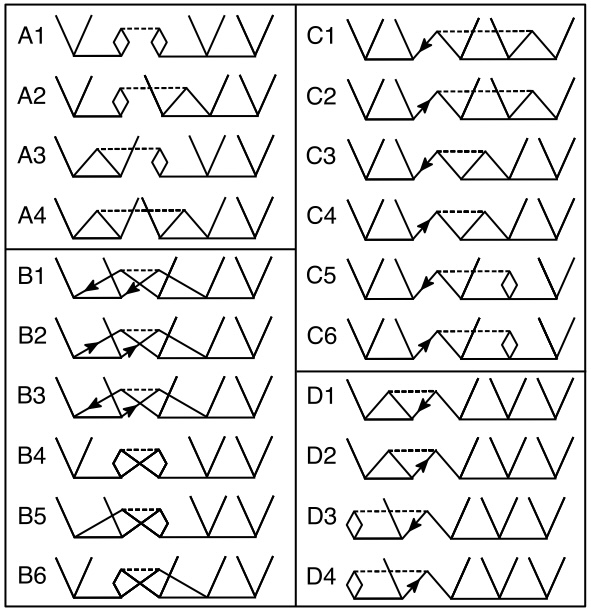
\includegraphics[width=6cm]{T2T3Diagrams.jpeg}
  %\rule[0.5em]{23.5em}{0.5pt}
  \caption{Spin-summed diagrams of $\op T_2\op T_3$ contributions to the triples residuals in CCSDT.}
\label{fig:T2T3_diagrams}
\end{figure}
Classifying the spin-summed $\op T_2\op T_3$ diagrams contributing to the triples residuals 
into groups A, B, C, and D:
\begin{itemize}
\item Diagrams \textbf{A1--A4}: kept unchanged,
\item Diagrams \textbf{B1--B6}: fully removed,
\item Diagrams \textbf{C1--C6} and \textbf{D1--D4}: multiplied by $\half$.
\end{itemize}
This approximation preserves size-extensivity, particle-hole symmetry, 
exactness for three-electron (or three-hole) systems, and invariance 
to rotations within the occupied and virtual spaces.


\subsection{Residual equations in the SVD basis}
\label{sec:svd_residuals}

The bra-projection for the singles and doubles residual equations uses 
the contravariant CSFs. For the triples, the contravariant CSF is
\begin{equation}
  \widetilde{\Phi}_{abc}^{ijk} = \Phi_{abc}^{ijk} - \Phi_{cab}^{ijk}.
\end{equation}
Due to the overlap properties of this choice the full triples residual has the structure
\begin{equation}
  \bar{R}^{ijk}_{abc} = R^{ijk}_{abc} - R^{ijk}_{cab} = \mathcal{A}(abc,cab)\, R^{ijk}_{abc},
\end{equation}
where $\mathcal{A}(abc,cab)F(a,b,c) = F(a,b,c) - F(c,a,b)$.
Since $R^{ijk}_{abc} = 0$ implies $R^{ijk}_{cab} = 0$, it is sufficient to solve 
$R^{ijk}_{abc} = 0$ with only half the terms.

\subsubsection{Triples contributions to the singles residual}

The triples contributions to the singles residual read:
\begin{equation}
\begin{aligned}
R_a^i &\leftarrow U_a^{iX} \left[T_{XYZ} \left(2A^{YL} A^{ZL} - B^{YZ}\right)\right]
- U_a^{jY} \Big[2 {B}_{j}^{iXL} V_{XY}^{L}- G_{jY}^{i}\Big],
\end{aligned}
\end{equation}
with intermediates
\begin{equation}
\begin{aligned}
A^{XL}&={B}_{i}^{iXL}, &{B}_{i}^{jXL} &= v_i^{aL} U_a^{jX},\\
B^{XY}&={B}_{i}^{jXL} {B}_{j}^{iYL}, 
&w_k^{dX} &= v_l^{dL} {B}_k^{lXL},\\
V_{XY}^{L} &= T_{XYZ} A^{ZL}, &G_{jY}^{i} &= T_{dYZ}^{i} w_j^{dZ},\\
T_{aYZ}^{i} &= T_{XYZ} U_a^{iX}. &
\end{aligned}
\end{equation}

\subsubsection{Triples contributions to the doubles residual}

\begin{equation}
\begin{aligned}
R_{ab}^{ij} &\leftarrow \sop{ij,ab} \Big\{ 
- \left(\bar B_a^{iLZ} - B_a^{iLZ}\right) V_{bZ}^{jL}
+U_b^{jZ} \Big[2\left(\bar B_a^{iLY} - B_a^{iLY}\right) V_{YZ}^{L} \\
& + T_{aYZ}^{i} \left(\hat{f}_k^c U_c^{kY}\right)
  - T_{XYZ} \left(U_c^{iY}\left(\bar B_a^{kLX} v_k^{cL}\right) 
- U_a^{kY} \left(B_c^{iLX} v_k^{cL} - \hat{f}_k^c U_c^{iX}\right)\right)\Big]
 \Big\},
\end{aligned}
\end{equation}
with intermediates
\begin{equation}
\begin{aligned}
B_a^{iLX} &= \hat{v}_j^{iL} U_a^{jX},  &\bar B_a^{iLX} &= \hat{v}_a^{bL} U_b^{iX},\\
V_{bZ}^{jL} &= {B}_k^{jYL} T_{bYZ}^{k}, &
\end{aligned}
\end{equation}
and the symmetrization operator $\sop{ij,ab}  X_{ab}^{ij} = X_{ab}^{ij} + X_{ba}^{ji}$.

\subsubsection{Triples residual}

The triples residual equations in the SVD basis read:
\begin{equation}
  R_{XYZ} = Q_{XYZ} + Q_{YXZ} + Q_{XZY} + Q_{ZYX} + Q_{ZXY} + Q_{YZX}
   + q_{XYZ} + q_{YXZ} + q_{ZYX}
\end{equation}
with the main intermediates
\begin{equation}
\begin{aligned}
  Q_{XYZ} &= U^{\dagger b}_{jY} \Big[T_{bX}^l X_{lZ}^j - X_{bZ}^d T_{dX}^j 
  +T_{bY'Z}^{l} \left(U_d^{jY'}  \left(v_l^{dL} Y_X^L \right)\right)\Big]
\end{aligned}
\end{equation}
and
\begin{equation}
\begin{aligned}
  q_{XYZ} &= T_{X'YZ} \Big[U^{\dagger a}_{iX} \Big( \left(\hat{f}_l^i + \half v_l^{dL} V_d^{iL}\right)U_a^{lX'}
  - \left(\hat{f}_a^d - \half v_l^{dL} V_{a}^{lL}\right) U_d^{iX'}\\
 & + \left(\hat{v}_l^{iL} \hat{v}_a^{dL}\right) U_d^{lX'}\Big)
 -2 Y_X^L A^{X'L}\Big]
  - T_{XY'Z'} \left( W_Y^{Y'L} W_Z^{Z'L}\right).
\end{aligned}
\end{equation}
The further intermediates used in these expressions are 
\begin{equation}
\begin{aligned}
X_{bZ}^d &= \hat{v}_b^{dL} Y_Z^L - \hat{f}_l^d T_{bZ}^l 
 - U^{lX}_{b} \left(v_l^{dL} \tilde V_{ZX}^{L}\right)
 + \left(\hat v_{lk}^{di} T^{lk}_{ba} - \hat v_{la}^{dc} T^{li}_{bc}\right) U^{\dagger a}_{iZ}
- \hat v_{lb}^{dc} T_{cZ}^l 
 + \half T_{bYZ}^{k} w_k^{dY},
\end{aligned}
\end{equation}

\begin{equation}
\begin{aligned}
X_{lZ}^j&= \hat{v}_l^{jL} Y_Z^L
 + U^{jX}_{d} \left(v_l^{dL} \tilde V_{ZX}^{L}\right) 
 + \left(\hat v_{la}^{dc} T^{ji}_{dc} - \hat v_{lk}^{di} T^{jk}_{da}\right) U^{\dagger a}_{iZ}
  - \hat v_{lk}^{dj} T^k_{dZ}
  - \half G_{lZ}^{j},
\end{aligned}
\end{equation}
and
\begin{equation}
\begin{aligned}
  &V_a^{iL} = v_k^{cL}  \widetilde{T}_{ac}^{ik}, &
  Y_X^L &= U^{\dagger a}_{iX} \left(\hat{v}_a^{iL} + V_a^{iL} \right),\\
&T_{aX}^i = U^{\dagger b}_{jX}  T_{ab}^{ij}, &
\widetilde{T}_{ab}^{ij} &= 2  T_{ab}^{ij} - T_{ba}^{ij},\\
&\hat v_{la}^{dc} = v_l^{dL} \hat v_a^{cL}, &
\hat v_{lk}^{di} &= v_l^{dL} \hat v_k^{iL},\\
&W_{Y}^{Y'L} =  U^{\dagger b}_{jY}  \left(\bar B_b^{jLY'} - B_b^{jLY'}\right), &
\tilde V_{ZX}^{L} &= V_{ZX}^{L} - \half V_{cX}^{kL} U^{\dagger c}_{kZ}.
\end{aligned}
\end{equation}

None of the contractions above involve more than six different indices.
This means that the tensor decompositions reduce the scaling of the DC-CCSDT method 
from ${\cal O}(N^8)$ to ${\cal O}(N^6)$, provided the number of SVD basis functions 
grows linearly with the system size.
The most expensive terms in the SVD-DC-CCSDT residual equations scale as $N_o^2 N_v N_X^2 N_L$,
where $N_o$ and $N_v$ are the numbers of occupied and virtual orbitals,
and $N_X$ and $N_L$ are the numbers of SVD and density-fitting basis functions.

\subsubsection{Projected intermediates}

An additional approximation can be introduced by calculating the $V_{aX}^{iL}$ intermediate 
in an SVD basis, which reduces the scaling of the most expensive terms to $N_o^2 N_v N_X^3$:
\begin{equation}
\begin{aligned}
  V_{aX}^{iL} &\approx \bar V_{X\tilde Z}^{L} \tilde U^{i\tilde Z}_{a},\\
  \bar V_{X\tilde Z}^{L} &= \left(\left(\tilde U^{\dagger b}_{j\tilde Z} U^{kY}_{b} \right) T^{j}_{cXY}\right) v_k^{cL}.
\end{aligned}
\end{equation}
The $\tilde Z$ SVD space covers both the triples SVD space (for the $\tilde V_{XZ}^L$ intermediate)
and the doubles space (for the $\tilde U^{i\tilde Z}_a$ projection in the doubles residual equations).
It is constructed by expanding the triples SVD space by important orthogonal contributions 
from the doubles SVD space.


\subsection{Construction of the SVD basis}
\label{sec:svd_basis}

The construction of the singular vectors $U^{iX}_{a}$ must also scale as ${\cal O}(N^6)$.
This is achieved using a two-step procedure.

\subsubsection{Step 1: Doubles SVD basis}

First, the relevant block of an approximate two-particle density matrix is obtained from 
converged CCSD doubles amplitudes:
\begin{equation}
\mathcal{D}^{aj}_{ib} = T^{\dagger ac}_{ik} T^{jk}_{bc},
\end{equation}
and eigendecomposed:
\begin{equation}
\mathcal{D}^{aj}_{ib} \approx \bar{U}_{i\tilde{\bar X}}^{\dagger a} \bar{D}_{\tilde{\bar X}}
\bar{U}^{j\tilde{\bar X}}_{b}.
\end{equation}
The SVD basis $\{\tilde{\bar X}\}$ is truncated by disregarding eigenvectors 
with eigenvalues smaller than a threshold: $\bar{D}_{\tilde{\bar X}} \lt \varepsilon_{T2}$.

The basis is canonicalized by diagonalizing the Fock matrix in the SVD basis:
\begin{equation}
f_{\tilde{\bar X}}^{\tilde{\bar Y}}=\bar{U}_{i\tilde{\bar X}}^{\dagger a}
(\epsilon_a - \epsilon_i)\bar{U}^{i\tilde{\bar Y}}_{a}.
\end{equation}
In the basis of its eigenvectors $U_{\tilde{\bar X}}^{\bar{X}}$ the Fock matrix is diagonal, 
$f^{{\bar X}}_{{\bar Y}}=\epsilon_{\bar X}\delta^{{\bar X}}_{{\bar Y}}$,
and the complete transformation to the ${\bar X}$-basis is given by
\begin{equation}
\bar{U}^{i{\bar X}}_{a}=\bar{U}^{i\tilde{\bar X}}_{a}\bar{U}_{\tilde{\bar X}}^{\bar{X}}.
\end{equation}

\subsubsection{Step 2: Triples SVD basis via CC3-type density matrix}

Having the transformation matrices to the doubles SVD basis, 
a partially decomposed CC3-type triples residual is computed:
\begin{equation}
\begin{aligned}
  R^i_{a\bar X\bar Y} &= \left( X_{b\bar X}^{jL} \bar{U}^{\dagger b}_{j \bar Y} \right) \hat{v}_a^{iL} 
  + V_{a \bar X}^d T^i_{d \bar Y} - V^i_{l \bar X} T^l_{a \bar Y}
  + E^d_{l \bar X \bar Y} T_{ad}^{il},
\end{aligned}
\end{equation}
with intermediates
\begin{equation}
\begin{aligned}
  X_{b\bar X}^{jL} &= T^j_{c\bar X} \hat v_{b}^{cL} - T^l_{b\bar X} \hat v_{l}^{jL}, &
  T_{a \bar X}^i &= \bar{U}^{\dagger b}_{j \bar X} T^{ij}_{ab}, \\
  E^d_{l \bar X \bar Y} &= V_{a \bar X}^d \bar{U}_{l \bar Y}^{\dagger a} - V_{l \bar X}^{i} \bar{U}_{i \bar Y}^{\dagger d}, &
  W_{\bar X}^L &= \hat{v}_c^{kL} \bar{U}^{\dagger c}_{k \bar X}, \\
  V^d_{a \bar X} &= \hat{v}_a^{dL} W^L_{\bar X}, &
  V^j_{l \bar X} &= \hat{v}^{jL}_l W^L_{\bar X}.
\end{aligned}
\end{equation}
The last term of the residual scales as $N^6$, while all other terms scale as $N^5$.
Since the SVD basis is canonicalized, the partially transformed triples amplitudes 
are readily available:
\begin{equation}
T^i_{a\bar X\bar Y} = - \frac{R^i_{a\bar X\bar Y} + R^i_{a\bar Y\bar X}}{\epsilon_{\bar X} + \epsilon_{\bar Y} + \epsilon_{a} - \epsilon_{i}}.
\end{equation}
The triples two-particle density matrix is then computed as
\begin{equation}
  D^{aj}_{ib} = T^{\dagger a \bar X\bar Y}_{i} T_{b \bar X\bar Y}^{j}
\end{equation}
at $N^6$ cost.

The triples amplitudes in the SVD basis implicitly include nonphysical 
components with triply repeated occupied orbital indices (e.g., $T_{abc}^{iii}$),
which would cancel in case of a full SVD basis. 
Their contributions to the density matrix can be explicitly isolated and removed:
\begin{equation}
\begin{aligned}
  \Delta D^{aj}_{ib} &= (T^{\dagger a}_{i \bar X \bar Y} \mathcal{U}^{\bar X}_{i \bar X'} \mathcal{U}^{\bar Y}_{i\bar Y'}) T^{j \bar X' \bar Y'}_{b},\\
  \mathcal{U}^{\bar X }_{i\bar X'} &= \bar U^{\dagger a}_{i \bar X'} \bar U^{i \bar X}_{a},\\
  \widetilde{D}^{aj}_{ib} &= D^{aj}_{ib} - \left(1 - \half\delta^i_j \right) \sop{ij,ab} \Delta D^{aj}_{ib}.
\end{aligned}
\end{equation}

Finally, the actual SVD basis for the triples in DC-CCSDT is obtained by 
diagonalizing the corrected triples two-electron density matrix:
\begin{equation}
\widetilde{D}^{aj}_{ib} \approx U^{\dagger a}_{i \tilde{X}} D_{\tilde{X}}
U^{j\tilde{X}}_{b}.
\end{equation}
Eigenvectors with eigenvalues smaller than $\varepsilon_{T3}$ are discarded.
The SVD basis is again canonicalized by diagonalizing the Fock matrix,
\begin{equation}
f_{\tilde{X}}^{\tilde{Y}}=U_{i\tilde{X}}^{\dagger a}
(\epsilon_a - \epsilon_i)U^{i\tilde{Y}}_{a},
\end{equation}
and the final SVD transformation matrices are
\begin{equation}
U^{iX}_{a}=U^{i\tilde{X}}_{a} U_{\tilde{X}}^{X}.
\end{equation}

\subsubsection{Additional SVD basis for the projection approximation}

The additional SVD basis for the projection approximation 
is constructed by half-transforming the contravariant doubles amplitudes 
$\widetilde{T}^{ij}_{ab}$ to the SVD basis, projecting the part not covered 
by the triples SVD space:
\begin{equation}
  \Delta \widetilde{T}^{ij}_{ab} = \widetilde{T}^{ij}_{ab} - U^{iX}_{a} U^{\dagger c}_{kX} \widetilde{T}^{kj}_{cb},
\end{equation}
computing SVD of $\Delta \widetilde{T}^{ij}_{ab}$, and selecting the most important left vectors 
$\Delta U^{i\bar X}_a$, which are then added to the triples SVD basis.
A symmetric orthogonalization of the combined space is performed at the end.

\subsection{Amplitude update and convergence}

The eigenvalues $\epsilon_{X}$ of the Fock matrix in the SVD basis are employed 
in the amplitude update, carried out directly in the SVD basis:
\begin{equation}
\Delta T_{XYZ} = -\frac{R_{XYZ}}{\epsilon_X + \epsilon_Y + \epsilon_Z}.
\end{equation}
To accelerate convergence, DIIS is employed for singles, doubles, and triples amplitude vectors.

\subsection{Truncation thresholds}

The truncation of the SVD spaces is governed by two tolerances:
$\varepsilon_{T3}$ for the triples and $\varepsilon_{T2}$ for the auxiliary 
doubles SVD. 
These are linked by a weight factor $w_{T2}$:
\begin{equation}
\varepsilon_{T2}=w_{T2}\,\varepsilon_{T3}.
\end{equation}
The choice of $\varepsilon_{T2}$ has very little effect on the results provided 
it is not larger than $\varepsilon_{T3}$.

A hybrid approach with an SVD-error correction at the CCSD(T) level can be used 
to accelerate convergence with the SVD truncation threshold:
\begin{equation}
  E_{\textrm{DC-CCSDT}} \approx E_{\textrm{SVD-DC-CCSDT}}  + \delta_{\rm SVD},
\end{equation}
with
\begin{equation}
  \delta_{\rm SVD}=E_{\textrm{CCSD(T)}} - E_{\textrm{SVD-CCSD(T)}}.
\end{equation}


\subsection{Correlation energy}
The correlation energy is calculated using the singles and doubles amplitudes:
\begin{equation}
E= \left(2 T_a^i T_b^j - T_b^i T_a^j\right) v_{ij}^{ab} + 2 T_a^i f^a_i
+ (2T_{ab}^{ij} - T_{ba}^{ij}) v_{ij}^{ab}.
\end{equation}

\subsection{Scaling summary}
\begin{itemize}
\item \textbf{Full DC-CCSDT}: $\mathcal{O}(N^8)$.
\item \textbf{SVD-DC-CCSDT}: $\mathcal{O}(N^6)$, provided the number of SVD basis functions 
grows linearly with system size (confirmed by tests on alkane chains).
\item The most expensive terms in SVD-DC-CCSDT scale as $N_o^2 N_v N_X^2 N_L$.
Assuming $N_v \approx N_X$, these terms are only a factor of $N_L/N_v$ more expensive than the 
most expensive term in CCSD.
\item The 4-external ladder diagram of the triples is reduced to $N^5$.
\item The SVD-error and the size of the SVD bases scale linearly with system size, 
  confirming size extensivity.
\end{itemize}


\chapter{Full Configuration Interaction and Selected CI Methods}
\label{ch:fci}

\section{Introduction}

Full Configuration Interaction (FCI) provides the exact solution to the time-independent 
Schr\"odinger equation within a given orbital basis set. While FCI is the ultimate benchmark 
for quantum chemistry calculations, its exponential scaling with system size
limits its applicability to small systems.
This chapter describes the implementation of FCI and selected CI methods in \elemcoil,
including Heat-bath CI (HCI), multi-state calculations, P-space enhanced Davidson solver,
and reduced density matrix calculations.

\section{Full Configuration Interaction}
\label{sec:fci}

\subsection{Determinantal Representation}

A Slater determinant $|\Phi_I\rangle$ is specified by occupation numbers for each spin-orbital.
In the Knowles-Handy algorithm\cite{knowles84_fci}, determinants are represented separately 
for $\alpha$ and $\beta$ spins:
\beq
|\Phi^I\rangle = |\alpha^I\rangle \otimes |\beta^I\rangle
\eeq
where $|\alpha^I\rangle$ and $|\beta^I\rangle$ are strings of occupied spin-orbitals.

The FCI wave function is expanded as:
\beq
|\Psi\rangle = c_I |\Phi^I\rangle
\eeq
where $c_I$ are the CI coefficients to be determined.

\subsection{Slater-Condon Rules}

Matrix elements $\langle \Phi_I | \op{H} | \Phi^J \rangle$ can be evaluated using 
Slater-Condon rules:

\textbf{Identical determinants} ($|\Phi^I\rangle = |\Phi^J\rangle$):
\beq
\langle \Phi_I | \op{H} | \Phi^I \rangle = \sum_{i \in I} h_i^i 
    + \frac{1}{2} \sum_{i,j \in I} \left[ v_{ij}^{ij} - v_{ij}^{ji} \right]
\eeq

\textbf{Single excitation} ($|\Phi^J\rangle = \op{a}^\dagger_a \op{a}_i |\Phi^I\rangle$):
\beq
\langle \Phi_I | \op{H} | \Phi^J \rangle = \sgn_{ia} \left[ h_{a}^{i} 
    + \sum_{j \in I} \left[ v_{aj}^{ij} - v_{aj}^{ji} \right] \right]
\eeq
where $\sgn_{ia}$ is the fermionic phase factor from orbital reordering.

\textbf{Double excitation} ($|\Phi^J\rangle = \op{a}^\dagger_a \op{a}^\dagger_b \op{a}_j \op{a}_i |\Phi^I\rangle$):
\beq
\langle \Phi_I | \op{H} | \Phi^J \rangle = \sgn_{iajb} \left[ v_{ab}^{ij} - v_{ba}^{ij} \right]
\eeq

\textbf{Higher excitations}: Matrix elements vanish for determinants differing by more than 
two orbitals.

\subsection{String-Based Algorithm}

The Knowles-Handy algorithm\cite{knowles84_fci} evaluates the matrix-vector product 
$\vect{v}_{\text{out}} = \op{H} \vect{c}_{\text{in}}$ efficiently using string-based 
techniques and resolution of identity:

\beq
v_I = H_{I}^{J} c_J = \langle \alpha_I \beta_I | \op{H} | \alpha^J \beta^J \rangle c_J
\eeq

For the two-electron part of the Hamiltonian, we have:
\beq
\langle I| \half v_{pq}^{rs} \left(\op E^{p}_{r} \op E^{q}_{s} - \op E^{p}_{s}\delta^{q}_{r} \right)| J \rangle c_J,
= \half v_{pq}^{rs} \langle I | \op E^{p}_{r} |K><K| \op E^{q}_{s} | J \rangle c_J - \cdots,
\eeq

The Hamiltonian is decomposed into one-electron and two-electron parts:
\beq
\op{H} = \op{H}_1^{(\alpha)} + \op{H}_1^{(\beta)} 
       + \op{H}_2^{(\alpha\alpha)} + \op{H}_2^{(\beta\beta)} + \op{H}_2^{(\alpha\beta)}
\eeq

The one-electron part is absorbed into the two-electron integrals.
For remaining components, string substitutions are performed:
\begin{itemize}
\item \textbf{Same-spin two-electron}: Substitution in one string, sum over other string
\item \textbf{Opposite-spin two-electron}: Substitution in both strings simultaneously
\end{itemize}



\section{Davidson Iterative Diagonalization}
\label{sec:davidson}

\subsection{Davidson Algorithm}

The Davidson method finds the lowest eigenvalues of large matrices 
without explicit matrix construction. Given initial guess vectors $\{\vect{u}^1, \ldots, \vect{u}^k\}$,
the algorithm iteratively builds a subspace and solves:

\beq
\mat{H}_{\text{sub}} \vect{c} = E \vect{c},
\eeq
where $[\mat{H}_{\text{sub}}]_{i}^{j} = \langle \vect{u}_i | \op{H} | \vect{u}^j \rangle$.

\subsection{Subspace Expansion}

The residual vector for eigenstate $\st{n}$ is:
\beq
\vect{r}^{\st{n}} = \mat{H} \vect{x}^{\st{n}} - E^{\st{n}} \vect{x}^{\st{n}},
\eeq
where $\vect{x}^{\st{n}} = c_{i}^{\st{n}} \vect{u}^i$ is the approximate eigenvector.

A correction vector $\vect{u}^{\st{n}} \rightarrow \vect{u}^{k+1}$ is computed and added to the subspace. 
In \elemcoil, we use either the diagonal preconditioner,
\beq
u^\st{n}_{I} = \frac{r^\st{n}_{I}}{E^\st{n} - H_{I}^{I}},
\label{eq:diag_precond}
\eeq
or the P-space enhanced preconditioner (see \sect{sec:jacobi_davidson} and \sect{sec:pspace}).
\subsection{Jacobi-Davidson Preconditioner}
\label{sec:jacobi_davidson}

For improved convergence, especially for excited states, we implement the Jacobi-Davidson 
correction. The correction vector $\vect{u}^{\st{n}}$ solves:

\beq
(\mat{I} - \vect{x}^{\st{n}} \vect{x}_\st{n}^\dagger)(\mat{H} - E^\st{n})
(\mat{I} - \vect{x}^\st{n} \vect{x}_\st{n}^\dagger) \vect{u}^\st{n} 
= -\vect{r}^{\st{n}\perp},
\eeq
where $\vect{x}^{\st{n}}$ is the normalized Ritz vector and $\vect{r}^{\st{n}\perp}$ is the residual 
orthogonalized to $\vect{x}^{\st{n}}$.

In our implementation, we use a P-Q space decomposition where P is a selected subspace 
of important determinants and Q is its complement. For the Q space we use the simple diagonal preconditioner, \eq{eq:diag_precond}, 
while for the P space we solve the Jacobi-Davidson equation exactly, including the coupling to Q space.
The correction equation becomes:

\beq
\left[(\mat{I}_{\{P\}} - \vect{x}^\st{n}_{\{P\}} \vect{x}_{\st{n}\{P\}}^\dagger)(\mat{H}_{\{P\}} - E^\st{n})
(\mat{I}_{\{P\}} - \vect{x}^\st{n}_{\{P\}} \vect{x}_{\st{n}\{P\}}^\dagger) 
+ \alpha \vect{x}^\st{n}_{\{P\}} \vect{x}_{\st{n}\{P\}}^\dagger\right] \vect{u}^\st{n}_{\{P\}} = -\vect{r}_{\{P\}}^{\st{n}\perp} + \vect{s}_{\{P\}},
\eeq
with coupling terms:
\begin{align}
\alpha &= \vect{x}_{\st{n}\{Q\}}^\dagger (\mat{H}_{\{Q\}} - E^\st{n}) \vect{x}^{\st{n}}_{\{Q\}} \\
\vect{s}^\st{n}_{\{P\}} &= (\mat{I}_{\{P\}} - \vect{x}^\st{n}_{\{P\}} \vect{x}_{\st{n}\{P\}}^\dagger)
\left(\mat{H}_{\{P\}} - E^\st{n}\right)\vect{x}^\st{n}_{\{P\}}
  \left(\vect{x}_{\st{n}\{Q\}}^\dagger \vect{u}^{\st{n}}_{\{Q\}}\right) + \beta \vect{x}^\st{n}_{\{P\}} \\
\beta &= \vect{x}_{\st{n}\{Q\}}^\dagger(\mat{H}_{\{Q\}} - E^\st{n})
(\mat{I}_{\{Q\}} - \vect{x}^\st{n}_{\{Q\}} \vect{x}_{\st{n}\{Q\}}^\dagger)\vect{u}^\st{n}_{\{Q\}}.
\end{align}
Since $\mat{H}_{Q}$ is diagonal, $\alpha$ and $\beta$ are computed efficiently using only 
diagonal elements.

The equation is solved using a direct linear solver (LU or QR decomposition) since the P space is small.

\subsection{Multi-State Davidson}

For computing multiple states simultaneously, the algorithm is extended to maintain 
orthogonality between states. The subspace is expanded for all states:

\beq
\mat{H}_{\text{sub}} \mat{C} = \mat{C} \mat{E},
\eeq
where $\mat{E} = \text{diag}(E^\st{1}, E^\st{2}, \ldots, E^\st{n})$ and columns of $\mat{C}$ contain 
eigenvector coefficients.

\textbf{Dual convergence criteria}: Both energy convergence ($|\Delta E^\st{n}| \lt \epsilon_E$) 
and residual convergence ($\|\vect{r}^\st{n}\| \lt \epsilon_R$) must be satisfied for all states 
to ensure correct excited state energies.


\subsection{P-Space Selection}
\label{sec:pspace}

The P-space is a subset of important determinants used to generate high-quality initial 
guess vectors and preconditioners. Determinants are selected by:

\textbf{Excitation level}: Include all determinants up to $n$-fold excitations from the 
Hartree-Fock reference.

\textbf{Energy criterion}: Select determinants with diagonal elements satisfying:
\beq
H_{I}^{I} - E_{\text{HF}} \lt \Delta E_{\text{threshold}}
\eeq

\textbf{Hybrid selection}: Combine excitation level and energy criteria.

\textbf{HCI-based selection}: Use Heat-bath CI (see \sect{sec:hci}) to select the 
most important determinants.

\section{Heat-bath Configuration Interaction (HCI)/CIPSI}
\label{sec:hci}

\subsection{Algorithm Overview}

Heat-bath CI (HCI)\cite{holmes16_hci} is a selected CI method that efficiently selects 
important determinants using selection inspired by heat-bath sampling.
An extension towards CIPSI\cite{huron73_cipsi} is also implemented.

The algorithm consists of three phases plus an extension towards CIPSI:

\textbf{Phase I} (Setup): Pre-compute sorted lists of double excitation matrix elements:
\beq
\text{For each } (p,q): \quad \{(r,s,H_{rs \leftarrow pq})\} 
    \text{ sorted by } |H_{rs \leftarrow pq}| \text{ (decreasing)}
\eeq

\textbf{Phase II}: Variational calculation in the current selected space:
\beq
\mat{H}_{\text{sel}} \vect{c} = E_{\text{var}} \vect{c}
\eeq

\textbf{Phase III} (Heat-Bath Selection): Generate candidate determinants connected to the variational 
space by $|H_{J}^I c_I| \gt \epsilon_h$:


For each determinant $|\Phi_I\rangle$ in the variational space:
\begin{itemize}
\item Generate single excitations with $|f_{i}^{a} c_I| \gt \epsilon_h$
\item Use pre-sorted lists to generate only double excitations with $|v_{ij}^{ab} c_I| \gt \epsilon_h$
\item Adaptive threshold: $\epsilon_{\text{adaptive}} = \epsilon_h / |c_I|$
\end{itemize}

\textbf{Phase IV} (Perturbative selection à la CIPSI): Select determinants corresponding to 
highest perturbative amplitudes:
\beq
\pre{^{pert}} c_J^2 \approx \frac{\left|\sum_{I \in \{|H_{J}^I c_I| \gt \epsilon_h\}} H^I_{J} c_I\right|^2}{(E_{\text{var}} - H^J_{J})^2} \gt \epsilon_p^2
\eeq
The sum runs only over determinants that have a large contribution to the $J$ determinant
according to the heat-bath criterion, and therefore can be calculated during the Phase III,
essentially at no extra cost.

Note that in Phase III, the candidates are generated only for the new determinants, however,
the $H_{J}^I c_I$ values are accumulated for all determinants in the variational space.

\subsection{Efficient Excitation Generation}

The key to HCI performance is the setup phase, which pre-computes and sorts excitation lists.
For restricted Hartree-Fock (RHF), store:
\beq
\text{double\_excitations}[(p,q)] = \{(r,s,H_{rs \leftarrow pq})\}_{\text{sorted}},
\eeq
where $H_{rs \leftarrow pq} = v_{pq}^{rs} - v_{pq}^{sr}$ is the antisymmetrized matrix element,
and $H_{rs \leftarrow pq} = v_{pq}^{rs}$ for $p,q$ of opposite spin.

For unrestricted Hartree-Fock (UHF), store separately:
\begin{itemize}
\item $\alpha$-$\alpha$ excitations: $v_{pq}^{rs} - v_{pq}^{sr}$
\item $\beta$-$\beta$ excitations: $v_{pq}^{rs} - v_{pq}^{sr}$
\item $\alpha$-$\beta$ mixed excitations: $v_{pq}^{rs}$
\end{itemize}

\subsection{Multi-State HCI/CIPSI}

For multi-state calculations, use \textbf{state-maximum selection}:
\beq
\pre{^{pert,max}}c_J^2 = \max_{\st{n}=\st{1},\ldots,\st{N}_{\text{states}}} \left[  
    \frac{\left|\sum_{I \in \text{var}\epsilon_h}H^I_{J} c^\st{n}_{I}\right|^2}{(E^\st{n}_{\text{var}} - H^J_{J})^2} \right]
\eeq

This ensures determinants important for \emph{any} state are included, preventing bias 
toward the ground state.


The initial guess is generated by diagonalizing a small-space Hamiltonian:
\beq
N_{\text{small}} = \max\left(100, \sqrt{N_{\text{target}}}, 5 N_{\text{states}}\right)
\eeq
with determinants selected using hybrid method (energy + excitation level), and diagonalized 
to get initial eigenvectors for all states. 
This prevents missing excited states due to poor initialization.

  \subsection{Hamiltonian Matrix Construction}
The Hamiltonian matrix in the selected space is constructed using the Slater-Condon rules
(see \sect{sec:fci}) and stored in a sparse format 
(for each row, store only non-zero elements and their column indices).

The connections between determinants are identified using three helper lists 
(similar to Ref.~\cite{sharma_semistochastic_2017}):
\begin{itemize}
\item \textbf{Same alpha list}: For each alpha string, store all indices of determinants sharing that alpha string.
This list is used to find beta single and double excitations efficiently.
\item \textbf{Same beta list}: For each beta string, store all indices of determinants sharing that beta string.
This list is used to find alpha single and double excitations efficiently.
\item \textbf{Single alpha excitation list}: For each alpha string, store all alpha strings reachable by a single excitation.
This list is used to find mixed alpha-beta double excitations efficiently.
\end{itemize}
Using these lists, a list of connected determinants $i$ for each determinant $j$ is generated
(for $i \lt j$) and used to compute and store the Hamiltonian matrix elements.



\subsection{Second-Order Energy Correction}
\label{sec:pt2}

The PT2 correction recovers dynamical correlation from determinants outside the variational 
space\cite{holmes16_hci}:

\beq
\Delta E_{\text{PT2}} = \sum_{K \notin \text{var}} 
    \frac{\left(\sum_{I \in \text{var}} H^I_{K} c_I\right)^2}{E_{\text{var}} - H^K_{K}},
\eeq
where $K$ runs over all determinants connected to the variational space but not included in it.

To compute PT2 efficiently, adaptive thresholding is employed. For each variational determinant $|\Phi^I\rangle$,
\beq
\epsilon_{\text{adaptive}} = \frac{\epsilon_{pt2}}{|c_I|},
\eeq
and only excitations are generated with $|H_{K}^{I}| \gt \epsilon_{\text{adaptive}}$ using pre-sorted lists from setup.

In order to reduce memory usage, an additional layer of thresholding is applied during PT2 calculation.
This involves discarding excitations with small contributions before they are fully generated.
For this purpose, the instantaneous PT2 amplitudes are calculated as $H_{K}^{I} c_I / (E_{\text{var}} - H_{K}^{K})$,
and excitations with amplitudes below a second threshold $\epsilon_{pt2}^c$ are not added to the 
list of candidates for PT2 correction. If the $K$ determinant is already present in the list, 
its amplitude is updated accordingly, otherwise an energy contribution of this instantaneous
excitation is added to the PT2 energy directly and also to the uncertainty estimate of the PT2 energy.

In practice, the calculation corresponds to the Phase III + Phase IV of the HCI selection
with a different (tight) threshold $\epsilon_{pt2}$.

\section{Reduced Density Matrices}
\label{sec:rdm}

\subsection{One-Particle Density Matrix}

The one-particle reduced spin-resolved density matrix (1-RDM) is:
\beq
\gamma^p_{q} = \langle \Psi | \op{a}^\dagger_p \op{a}_q | \Psi \rangle
            = c^{I*} c_J \langle \Phi_I | \op{a}^\dagger_p \op{a}_q | \Phi^J \rangle
\eeq

For separate spin components ($\spa{p},\spa{q}$ and $\spb{p},\spb{q}$ correspond 
to $\alpha$ and $\beta$ orbitals, respectively):
\beq
\gamma^{\spa{p}}_{\spa{q}} &= c^{I*} c_J \langle \alpha_I \beta_I | 
    \op{a}^\dagger_{\spa{p}} \op{a}_{\spa{q}} | \alpha^J \beta^J \rangle \\
\gamma^{\spb{p}}_{\spb{q}} &= c^{I*} c_J \langle \alpha_I \beta_I | 
    \op{a}^\dagger_{\spb{p}} \op{a}_{\spb{q}} | \alpha^J \beta^J \rangle
\eeq

\textbf{Properties}:
\begin{itemize}
\item Trace: $\trace(\gamma^{(\alpha)}) = N_{\alpha}$, $\trace(\gamma^{(\beta)}) = N_{\beta}$
\item Hermitian: $\gamma_{pq} = \gamma_{qp}^*$
\item Eigenvalues: Natural orbital occupations $0 \leq n_i \leq 2$
\end{itemize}

\subsection{Transition Density Matrix}

For different states $|\Psi_\st{m}\rangle$ and $|\Psi_\st{n}\rangle$:
\beq
\pre{_\st{m}^\st{n}}\gamma^p_{q} = \langle \Psi_\st{m} | \op{a}^\dagger_p \op{a}_q | \Psi^\st{n} \rangle
\eeq

Used for computing transition properties (e.g., oscillator strengths, transition dipole moments).

\subsection{Two-Particle Density Matrix}

The two-particle reduced (spin-resolved) density matrix (2-RDM) is:
\beq
\Gamma^{pq}_{rs} = \langle \Psi | \op{a}^\dagger_p \op{a}^\dagger_q \op{a}_s \op{a}_r | \Psi \rangle
\eeq

\textbf{Energy verification}:
\beq
E = h_p^q \gamma^p_q + \frac{1}{2} v_{pq}^{rs} \Gamma^{pq}_{rs} + E_{\text{nuc}}
\eeq

\subsection{Natural Orbitals}

Diagonalize the 1-RDM:
\beq
\gamma \vect{\phi}_i = n_i \vect{\phi}_i
\eeq
Natural orbital occupations $n_i$ indicate importance of orbitals. Used for:
\begin{itemize}
\item Active space selection 
\item Identifying multireference character
\end{itemize}


\chapter{Orbital localization and region fragments}

\section{Localized occupied orbitals}

The region workflow starts from localized occupied orbitals. In the default implementation, the valence occupied space is localized with the intrinsic bond orbital (IBO) functional
\begin{equation}
  \mathcal{L}_{\mathrm{IBO}} = \sum_i \sum_A \left(q_A^i\right)^p,
\end{equation}
with IAO charges
\begin{equation}
  q_A^i = \sum_{\mu \in A} \left|\langle \mathrm{IAO}_\mu | \phi_i \rangle\right|^2,
\end{equation}
where $A$ labels atoms, $i$ labels occupied orbitals, and $p=4$ by default.
The working IAOs are obtained from the occupied orbitals $C_{\mathrm{occ}}$ and the minimal-basis overlap blocks
\begin{equation}
  P_{12} = S^{-1} S_{12},
  \qquad
  B = S_{21} C_{\mathrm{occ}},
  \qquad
  D = S_{22}^{-1} B.
\end{equation}
Following the revised formulation from supplementary materials of Ref.~\cite{senjeanGeneralizationIntrinsic2021}, 
\elemcoil{} first builds the proto-IAOs
\begin{equation}
  A_{\mathrm{proto}} = P_{12} + \left(C_{\mathrm{occ}} - P_{12} D \left(B^\dagger D\right)^{-1}\right) B^\dagger,
\end{equation}
and then performs a metric L\"owdin orthogonalization,
\begin{equation}
  C_{\mathrm{IAO}} = A_{\mathrm{proto}}\left(A_{\mathrm{proto}}^\dagger S A_{\mathrm{proto}}\right)^{-1/2}.
\end{equation}
Only non-ghost minimal-basis functions are retained in this construction.
The localized occupied orbitals are related to the input occupied orbitals through a rotation matrix
\begin{equation}
  |\tilde \phi_i\rangle = \sum_j |\phi_j\rangle R_{ji}.
\end{equation}

Let $\mathcal{C}_{\mathrm{arg}}$ denote the explicit center list passed to \cmd{@region}, and let
$\mathcal{C}_{\mathrm{incl}}^{\mathrm{opt}}$ and $\mathcal{C}_{\mathrm{excl}}^{\mathrm{opt}}$ denote
\cmd{region.inclusive\_centers} and \cmd{region.exclusive\_centers}, respectively.
The effective center sets are
\begin{align}
  \mathcal{C}_{\mathrm{incl}} &=
  \begin{cases}
    \mathcal{C}_{\mathrm{incl}}^{\mathrm{opt}} \cup \mathcal{C}_{\mathrm{arg}}, & \cmd{region.mode = :inclusive}, \\
    \mathcal{C}_{\mathrm{incl}}^{\mathrm{opt}}, & \cmd{region.mode = :exclusive},
  \end{cases} \\
  \mathcal{C}_{\mathrm{excl}} &=
  \begin{cases}
    \mathcal{C}_{\mathrm{excl}}^{\mathrm{opt}}, & \cmd{region.mode = :inclusive}, \\
    \mathcal{C}_{\mathrm{excl}}^{\mathrm{opt}} \cup \mathcal{C}_{\mathrm{arg}}, & \cmd{region.mode = :exclusive}.
  \end{cases}
\end{align}
An occupied orbital is retained when it satisfies either the inclusive or the exclusive rule:
\begin{align}
  i \in \mathcal{F}_{\mathrm{occ}}^{\mathrm{incl}} &\iff \exists A \in \mathcal{C}_{\mathrm{incl}} : q_A^i \ge \tau_{\mathrm{occ}}, \\
  i \in \mathcal{F}_{\mathrm{occ}}^{\mathrm{excl}} &\iff \left(\exists A \in \mathcal{C}_{\mathrm{excl}} : q_A^i \ge \tau_{\mathrm{occ}}\right) \wedge
  \left(\forall B,\ q_B^i \ge \tau_{\mathrm{occ}} \Rightarrow B \in \mathcal{C}_{\mathrm{excl}}\right),
\end{align}
where $\tau_{\mathrm{occ}} =$ \cmd{region.occ\_charge\_thr}.
The selected occupied orbitals are written as fragment-inactive orbitals in the tagged dump.

\section{Fragment virtual orbitals from support-atom OPAOs}

In the non-pi workflow, the fragment virtual space is built from support-atom projected atomic orbitals.
If $\mathcal{C}_{\mathrm{all}} = \mathcal{C}_{\mathrm{incl}} \cup \mathcal{C}_{\mathrm{excl}}$, the support set is defined as
\begin{equation}
  \mathcal{S} = \mathcal{C}_{\mathrm{all}} \cup \left\{A\ \middle|\ \exists i \in \mathcal{F}_{\mathrm{occ}},\ q_A^i \ge \tau_{\mathrm{atom}}\right\},
\end{equation}
where $\tau_{\mathrm{atom}} =$ \cmd{region.atom\_charge\_thr}.

Let $C_v$ denote the canonical virtual orbitals and let $S_{\mathrm{AO},\mathcal{S}}$ denote the AO overlap columns corresponding to AO functions on support atoms.
The fragment PAOs are formed as
\begin{equation}
  C_{\mathrm{PAO}} = C_v C_v^\dagger S_{\mathrm{AO},\mathcal{S}}.
\end{equation}
Their overlap matrix is
\begin{equation}
  S_{\mathrm{PAO}} = C_{\mathrm{PAO}}^\dagger S C_{\mathrm{PAO}}.
\end{equation}
A locality-preserving factor $M$ is built such that
\begin{equation}
  M^\dagger S_{\mathrm{PAO}} M = I.
\end{equation}
Near-redundant directions of $S_{\mathrm{PAO}}$ --- those with eigenvalue below
$\mathtt{opaofac}\cdot\mathtt{redthr}\cdot\lambda_{\max}$ (\cmd{loc.opaofac} times the AO basis
redundancy threshold \cmd{scf.redthr}) --- are dropped, so $M$ has fewer columns than
$C_{\mathrm{PAO}}$ when the support PAOs are linearly dependent in the virtual space. The retained
PAOs are selected by a rank-revealing column-pivoted QR of the kept eigenvectors of
$S_{\mathrm{PAO}}$ and orthogonalized by a symmetric L\"owdin transformation (with one refinement
step), keeping the OPAOs local. This yields orthogonal PAOs
\begin{equation}
  C_{\mathrm{OPAO}} = C_{\mathrm{PAO}} M.
\end{equation}
The corresponding virtual rotation is obtained from
\begin{equation}
  R_{\mathrm{virt}} = C_v^\dagger S C_{\mathrm{OPAO}}.
\end{equation}

\section{Local pi axes and target orbitals}

For \cmd{region.pi = :occupied} or \cmd{:both}, one local target $p'_z$ orbital is constructed for each selected atom.
The bonding graph is built from the distance criterion
\begin{equation}
  r_{AB} \lt 1.3\left(R_A + R_B\right),
\end{equation}
where $R_A$ and $R_B$ are element-specific covalent radii.

For each selected atom $A$, a local plane neighborhood $\mathcal{P}_A$ is assembled from bonded neighbors first, with nearest-atom fallbacks if the bonded graph is insufficient to define a plane.
The code then constructs the symmetric matrix
\begin{equation}
  G_A = \sum_{B \in \mathcal{P}_A} \left(\vect{R}_B - \vect{R}_A\right)\left(\vect{R}_B - \vect{R}_A\right)^\dagger,
\end{equation}
and takes the normalized eigenvector corresponding to the smallest eigenvalue as the local plane normal $\vect{n}_A$.

If $|p_x^A\rangle$, $|p_y^A\rangle$, and $|p_z^A\rangle$ denote the highest-valence p-type IAOs on atom $A$, the target local pi orbital is
\begin{equation}
  |p'_{z,A}\rangle = n_{A,x}|p_x^A\rangle + n_{A,y}|p_y^A\rangle + n_{A,z}|p_z^A\rangle.
\end{equation}

\section{Pi-space projector}

Let $P_Z$ be the matrix whose columns are the target orbitals $|p'_{z,A}\rangle$ and let $C_{\mathrm{blk}}$ denote either the occupied or the virtual block under consideration.
The projected overlaps are
\begin{equation}
  X = P_Z^\dagger S C_{\mathrm{blk}},
  \qquad
  S_\pi = P_Z^\dagger S P_Z.
\end{equation}
\elemcoil{} diagonalizes the projector-overlap matrix
\begin{equation}
  O = X^\dagger S_\pi^{-1} X.
\end{equation}
If
\begin{equation}
  O U = U \Lambda,
\end{equation}
the rotated block is formed with eigenvectors ordered by descending eigenvalues, so the leading orbitals are those with the largest pi-projector overlap.

The automatic total number of local $\pi$ electrons is
\begin{equation}
  n_{\pi,e} =
  \begin{cases}
    \cmd{region.pi\_electrons}, & \text{if this option is set non-negative}, \\
    \sum\limits_{A \in \mathcal{C}_{\mathrm{all}}} n_{\pi,e}(A), & \text{otherwise},
  \end{cases}
\end{equation}
where the fallback atomic contributions $n_{\pi,e}(A)$ use an element- and coordination-based main-group $p$-block rule.

For restricted references, the default occupied and virtual $\pi$ counts are
\begin{equation}
  n_{\pi,\mathrm{occ}} = \frac{n_{\pi,e}}{2},
  \qquad
  n_{\pi,\mathrm{virt}} = N_{\mathrm{centers}} - n_{\pi,\mathrm{occ}}.
\end{equation}
These defaults can be overridden by \cmd{region.pi\_occupied} and \cmd{region.pi\_virtual}, in which case only the leading occupied and virtual projector-ordered orbitals are retained.
For unrestricted references, the alpha and beta occupied counts are split using the spin population difference $m_s^{(2)} = N_\alpha - N_\beta$,
\begin{equation}
  n_{\pi,\mathrm{occ}}^\alpha = \frac{n_{\pi,e} + m_s^{(2)}}{2},
  \qquad
  n_{\pi,\mathrm{occ}}^\beta = \frac{n_{\pi,e} - m_s^{(2)}}{2}.
\end{equation}

\section{Pseudo-canonicalization}

If \cmd{region.pseudo = true}, the selected fragment occupied and fragment virtual blocks are semicanonicalized by diagonalizing the corresponding Fock subblocks. For a fragment block $C_f$ this amounts to diagonalizing
\begin{equation}
  F_f = C_f^\dagger F_{\mathrm{AO}} C_f,
\end{equation}
and rotating the block with the eigenvectors of $F_f$.



\chapter{Automatically generated UCCSDT and UDC-CCSDT}
Unrestricted implementations of CCSDT and DC-CCSDT\cite{kats19_dc,rishi19,schraivogel21_dc} 
were generated with version 1.0.1 of the \quantwo\ program\cite{quantwo}.
The \quantwo\ inputs are listed below.
\begin{itemize}
  \item UCCSDT \quantwo\ input file:
\lstset{language=[LaTeX]Tex, frame=shadowbox, rulesepcolor=\color{gray}, basicstyle=\ttfamily\scriptsize, columns=fullflexible, breaklines=true}
\begin{lstlisting}
prog,spinintegr=0,nobrafac=1,explspin=1,algo=2
output,level=1,maxlenline=70

\beq
<\Phi^{a}_{i}| \op H (1 + \op T_2 + \op T_3) |0>_C
\eeq
\beq
<\Phi^{ab}_{ij}| \op H (1 + \op T_2 + \half \op T_2 \op T_2 + \op T_3) |0>_C
\eeq
\beq
<\Phi^{abc}_{ijk}| \op H (\op T_2 + \op T_3 + \half \op T_2 \op T_2 + \op T_2 \op T_3) |0>_C
\eeq
\end{lstlisting}
\item UDC-CCSDT \quantwo\ input file:
\begin{lstlisting}
%singles and doubles amplitude equations from UCCSDT
%we only modify the triples amplitude equation

prog,spinintegr=0,nobrafac=1,explspin=1,algo=2
output,level=1,maxlenline=70

\beq
<\Phi^{abc}_{ijk}| \op H (\op T_2 + \op T_3 + \frac{1}{2} \op T_2 \op T_2 
+ \op T_2 \op T_3) |0>_C 
+ (1 - \Perm{IJ}{JI} - \Perm{IK}{KI})(1 - \Perm{AB}{BA} - \Perm{AC}{CA})
(\sum_{LMDE} \tnsr \intg{LE}{MD} \tnsr T^{IL}_{AD} \tnsr T^{MJK}_{EBC}) 
- \frac{1}{2}(1 - \Perm{KI}{IK} - \Perm{KJ}{JK}) 
\sum_{LMDE} \tnsr \intg{LD}{ME} \tnsr T^{IJ}_{DE} \tnsr T^{LMK}_{ABC} 
- \frac{1}{2}(1 - \Perm{CA}{AC} - \Perm{CB}{BC}) 
\sum_{LMDE} \tnsr \intg{LD}{ME} \tnsr T^{LM}_{AB} \tnsr T^{IJK}_{DEC} 
+ \frac{1}{2}(1 - \Perm{IJ}{JI} - \Perm{IK}{KI}) 
\sum_{LMDE} \tnsr \intg{LD}{ME} \tnsr T^{LI}_{DE} \tnsr T^{MJK}_{ABC} 
+ \frac{1}{2}(1 - \Perm{AB}{BA} - \Perm{AC}{CA}) 
\sum_{LMDE} \tnsr \intg{LD}{ME} \tnsr T^{LM}_{DA} \tnsr T^{IJK}_{EBC} 
+ \frac{1}{2}(1 - \Perm{KI}{IK} - \Perm{KJ}{JK})(1 - \Perm{AB}{BA} - \Perm{AC}{CA}) 
\sum_{LMDE} \tnsr \intg{LD}{ME} \tnsr T^{IJ}_{AD} \tnsr T^{LMK}_{BEC} 
+ \frac{1}{2}(1 - \Perm{IJ}{JI} - \Perm{IK}{KI})(1 - \Perm{CA}{AC} - \Perm{CB}{BC}) 
\sum_{LMDE} \tnsr \intg{LD}{ME} \tnsr T^{IL}_{AB} \tnsr T^{JMK}_{DEC}
\eeq
\end{lstlisting}
\end{itemize}
\noindent The program generates \textsf{TensorOperations} code.
The generated code  used by \elemcoil\ is located in the \texttt{src/algo} directory. 
\addcontentsline{toc}{chapter}{Bibliography}
\bibliography{references.bib}
\bibliographystyle{naturemag}
\end{document}
